% Copyright (C)  2015  Philipp Hacker.
% Permission is granted to copy, distribute and/or modify this document
% under the terms of the GNU Free Documentation License, Version 1.3
% or any later version published by the Free Software Foundation;
% with no Invariant Sections, no Front-Cover Texts, and no Back-Cover Texts.
% The lincense itself can be found at <https://www.gnu.org/licenses/fdl-1.3>.

\documentclass[numbers=noenddot,a4paper]{scrartcl}

\usepackage[greek,ngerman]{babel}
\usepackage[T1]{fontenc}
%\usepackage[applemac]{inputenc}
\usepackage[utf8]{inputenc}
\usepackage{fullpage}
\usepackage{scrpage2}
\usepackage{libertine}
%\usepackage{braket}
\usepackage{ziffer}
\usepackage{graphicx}
\usepackage{units}
\usepackage[infoshow]{tabularx}
\usepackage[all]{xy}
\usepackage{amsmath}
\usepackage{amssymb}
\usepackage{wrapfig}
\usepackage{upgreek}
\usepackage{esint}
\usepackage{float}
\usepackage[font=small,labelfont=bf]{caption}
\usepackage{subcaption}
\usepackage{lscape}
\usepackage[backref=page]{hyperref}
\usepackage{csquotes}
\usepackage[printonlyused,withpage,footnote]{acronym}

\renewcommand{\thefigure}{Abb. \arabic{figure}}
%\renewcommand{\bflabel}[1]{\normalfont{\normalsize{#1}}\hfill}

%\captionsetup[wrapfigure]{name=}
\captionsetup[figure]{name=}

\newcommand{\nummat}[1]{\left[\text{#1}\right]}
\newcommand{\num}[1]{$\left[\text{#1}\right]$}
\newcommand{\degree}{^\circ}
\newcommand{\diff}{\textnormal{d}}
\newcommand{\tenpo}[1]{ 10^{#1}}
\newcommand{\greek}[1]{\greektext#1\latintext}
\newcommand{\ix}[1]{_\text{#1}}
\newcommand{\imag}{\mathbf{i}}
\newcommand{\tilt}[1]{\textit{#1}}
\newcommand{\grad}[1]{\textit{grad}\left(#1\right)}
\newcommand{\divergenz}[1]{\textit{div}\left(#1\right)}
\newcommand{\euler}{\mathnormal{e}}
\newcommand{\fett}[1]{\textbf{#1}}
\newcommand{\einnup}{\hspace{0.2cm}}
\newcommand{\einnum}{\hspace{-0.2cm}}
\newcommand{\zentriert}[1]{\begin{center}#1\end{center}}

\title{Bachelor-Arbeit zum Thema \enquote{Modenanregung in \tilt{Yukawa}-Bällen}} %TODO Name
\author{Philipp Hacker} %TODO Author
\date{\today}

\setcounter{section}{-1}

\begin{document}

	\maketitle

	\begin{center}

		Institut für Physik\\
		Mathematisch-Naturwissenschaftliche Fakultät\\
		Universität Greifswald

	\end{center}
	
	\vspace{0.5cm}

	\begin{figure}[H]
			\centering
			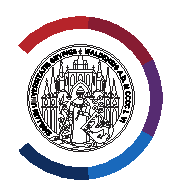
\includegraphics[width=0.35\textwidth]{figs/unilogo_NEU_schwarz.eps}
	\end{figure}

	\vspace{0.5cm}

	\begin{center}

			\hspace{-0.55cm} Erst-Gutachter: Prof. Dr. André Melzer \\ \vspace{0.25cm} %TODO Name Erst-Gutachter

			Zweit-Gutachter: Prof. Dr. Lutz Schweikhard \\ \vspace{0.25cm} %TODO Name Zweit-Gutachter

			Bearbeitungszeitraum: 01.03.2015 bis 12.07.2015 \\ \vspace{0.25cm} %TODO Bearbeitungszeitraum

%		\begin{table}[h]
%			\centering
%			Note (Erst-Gutachter): %TODO Gute Note erhalten :)
%			\begin{tabularx}{1.5cm}{|X|}
%				\hline \\ \\
%				\hline
%			\end{tabularx}
%			
%			\centering
%			\hspace{-0.42cm} Note (Zweit-Gutachter): %TODO Gute Note erhalten :)
%			\begin{tabularx}{1.5cm}{|X|}
%				\hline \\ \\
%				\hline
%			\end{tabularx}
%			
%		\end{table}

	\end{center}

	\thispagestyle{empty}

	\newpage
	\thispagestyle{empty}
	\begin{align*}
	\,
	\end{align*}
	\newpage

	\tableofcontents

	\newpage
	\thispagestyle{empty}
	\begin{align*}
	\,
	\end{align*}
	\newpage

	\section{Motivation}\label{sec:einleitung}

	\newpage

	\section{Physikalische Grundlagen}\label{sec:physg}

		In diesem ersten Abschnitt soll der Hintergrund f\"ur den sich anschlie{\ss}nenden Versuch gegeben werden. Dabei wird einerseits auf grundlegendes aus der Plasmaphysik sowie komplexer Plasmen eingegangen, andererseits aber auch auf die theoretischen Modelle, welche essentiell f\"ur das Verst\"andnis der Ph\"anomene dieses Experiments sind.

		\subsection{Kapazitiv gekoppelte Radiofrequenz-Plasmen} \label{sub:kaprfplasm}

			Der in diesem Versuch genutzte Aufbau entspricht dem eines kapazitiv gekoppelten Niederdruck-Radiofreuquenz-Plasmas.\\
			Ein Plasma ist ein quasineutrales Gas aus freien Ladungsträgern und, dem Ionisierungsgrad der Entladung entsprechend, neutralen Atomen oder Molekülen. Die Spezies der Ladungen sind im allgemeinen Elektronen und Ionen, wobei der Begriff quasineutral die Bedingung $n\ix{e}=n\ix{I}$ der Dichten auf einer speziellen Längenskala fordert (siehe unten). Für ein Plasma gibt es verschiedene physikalischen Kenngrößen, welche in Tabelle \ref{tab:kenngroessen} inklusive ihrer Bedeutungen einmal zusammengefasst wurden.\\
			Befindet sich ein Fremdteilchen, ein Festkörper oder eine weitere Ladungsträgerspezies in der Entladung, so spricht man von komplexen Plasmen. Für das Experiment dieser Arbeit ist dies der Fall, da hierbei in das Plasma homogene Melamin-Formaldehyd-Partikel in der Größenordnung einiger $\unit{\upmu m}$ eingebracht werden. Diese erfahren, in Abhängigkeit der Parameter, verschiedenste Wechselwirkungen mit den Entladungsspezies und externen Feldern.

				\begin{table}[H]
					\centering
						\begin{tabular}{m{0.3\textwidth}|m{0.3\textwidth}|m{0.3\textwidth}}
							Größe & Zusammenhang & Bedeutung \\ 
							\hline  Debye-Länge & $\lambda\ix{D,j}^2=\frac{\varepsilon\ix{0}k\ix{B}T\ix{j}}{n\ix{j}e^2}$
							\newline
							$\lambda\ix{D}^2=\left(\lambda\ix{D,e}^{-2}+\lambda\ix{D,I}^{-2}\right)^{-1}$ & die Distanz um eine Probeladung, ab welcher die Quasineutralität gilt\\ 

							\hline Plasmafrequenz & $\omega\ix{P,j}^2=\frac{n\ix{j}e^2}{\varepsilon\ix{0}m\ix{j}}=\frac{v\ix{th,j}}{\lambda\ix{D,j}}=\frac{1}{\tau\ix{j}}$ & obere Grenze der Zeitskala für die Wechselwirkung mit externen Kräften bzw. Feldern; Inverse der Abschirmungszeit \\ 

							\hline thermisches Geschwindigkeit & $v\ix{th,j}^2=\frac{k\ix{B}T\ix{j}}{m\ix{j}}$ & mittlere Geschwindigkeit aus der Definition der kinetischen Gastheorie \\ 

							\hline mittlerer Teilchenabstand & $\overline{b}=\frac{\hbar}{m\ix{j}v\ix{th,j}}$ & gemittelter Teilchenabstand (entspricht thermischer \mbox{\tilt{de-Broglie}-Wellenlänge}) \\ 

							\hline Yukawa-Potential & $\Phi=\frac{Q}{4\pi\varepsilon|\vec{r}|}\euler^{-\frac{|\vec{r}|}{\lambda\ix{D}}}$ & elektrostatisches Wechselwirkungspotential einer Probeladung $Q$ in einem Plasma \\

							\hline

						\end{tabular}
					\caption{Plasmaphysikalische Kenngrößen. Der Index $j$ bestimmt die Ladungsträgerspezies mit den entsprechenden Massen und Ladungen.}
					\label{tab:kenngroessen}
				\end{table}

			Wie bereits erwähnt greift dieses Experiment auf die Erzeugung einer Gasentladung zurück. Hierbei ist der Versuch wie ein horizontal ausgerichteter, paralleler Plattenkondensator angeordnet (siehe \ref{img:ungleichesplasma}), wobei das Dielektrikum das Plasma sei, die untere Elektrode mit einem Signal im $\unit{MHz}$-Bereich betrieben wird und die andere auf Massepotential liegt. Das elektrische Feld resultiert hierbei aus den Oberflächenladungen der Elektroden, wobei mit unterschiedlichen \tilt{rf}-Signalen (\tilt{radio frequency}) auch verschiedene Betriebsregime realisiert, e.g. Ladungsträger erzeugt bzw. vernichtet werden.\\
			Die \tilt{rf}-Spannung sorgt weiterhin für die nötige Homogenität des Plasmas, da aufgrund dessen ein Verschiebungsstrom zwischen Entladungsvolumen und Elektrode fließt (siehe Abschn. \ref{subsub:self-bias}) und damit die Kontaktierung dieser sehr isotrop gestaltet. In Aufbauten, in welchen die Flächen der Elektroden nicht gleich sind, liegt wegen der unterschiedlichen Potentialverläufe in den Randschichten (siehe Abschn. \ref{sub:rand}) zusätzlich eine Gleichspannung an, die sogenannte \tilt{self-bias} - siehe Abschn. \ref{subsub:self-bias}. Das ist insbesondere der Fall für das Experiment dieser Arbeit, da hier die gesamte Kammer als Elektrode zur Masse dient und die andere entsprechend kapazitiv an die Erregung gekoppelt ist.

				\subsubsection{Verschiebungsstrom} \label{subsub:verschieb}

					\begin{wrapfigure}{r}{0.4\textwidth}
						\centering
						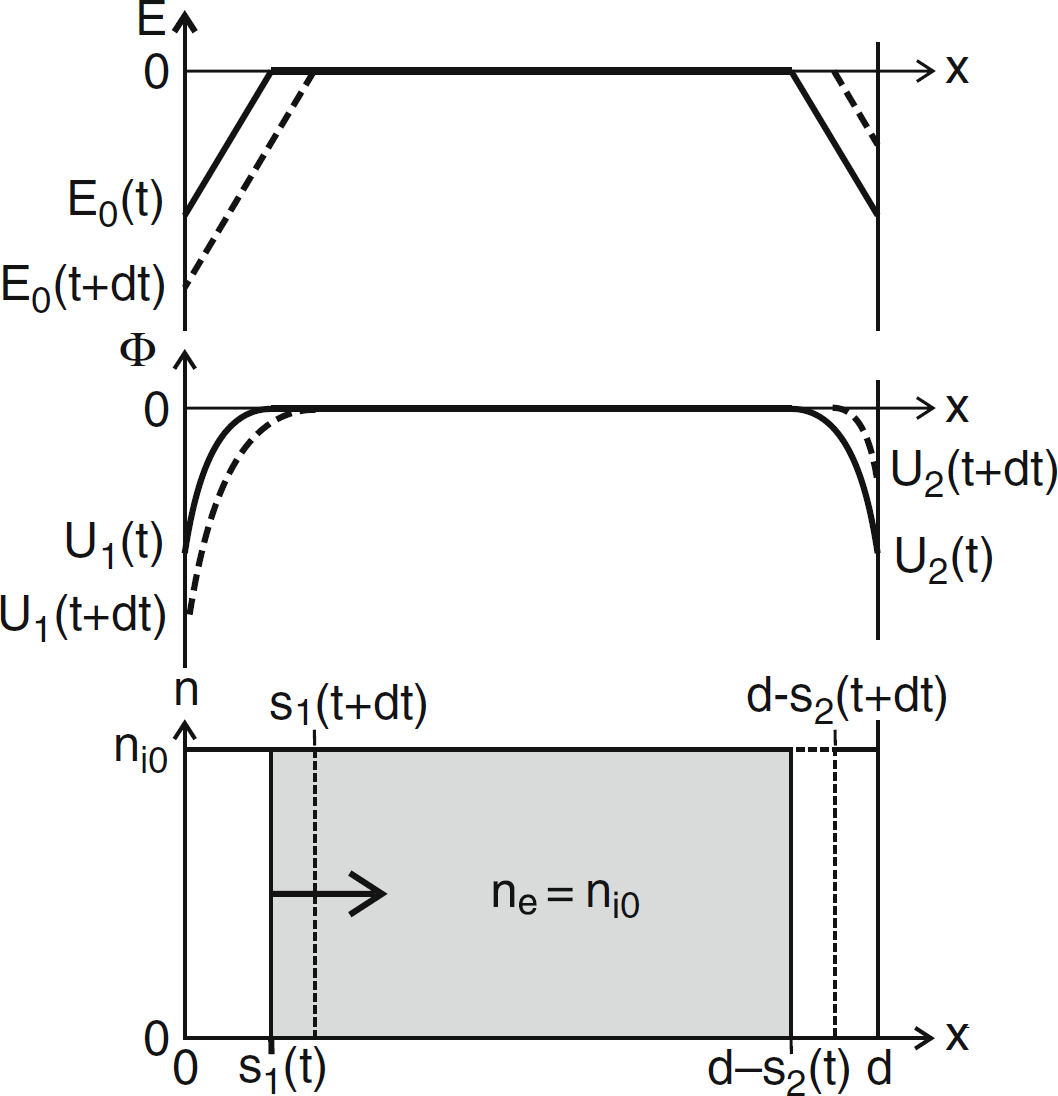
\includegraphics[width=0.47\textwidth,height=0.54\textwidth]{figs/verschiebpiel.png}
						\caption{Verlauf der Dichten, des Elektrischen Feldes und des zug. Potentials (eindimensional) in einer Entladung mit zwei gegenüberliegenden Randschichten (nach \cite{Piel10}).}
						\label{img:verschieb}
					\end{wrapfigure}

				Die Elektronen eines Plasmas über einer \tilt{rf}-getriebenen Elektrode können, aufgrund ihrer Beweglichkeit und hohen Plasmafrequenz $\omega\ix{P,e}$ der Anregung problemlos folgen. Die Ionen sollen in diesem Fall als stationär betrachtet werden, da $\omega\ix{P,I}\ll\omega\ix{P,e}\,$. Nimmt man an, dass die Randschicht der Dicke $a$ frei von Elektronen ist (siehe Abschn. \ref{sub:rand}) und die Ionendichte dort konstant $n\ix{0,I}$ ist, so folgt für das elektrische Feld der positiven Raumladungszone an der Kammerwand $E\ix{0}=-en\ix{0,I}a/\varepsilon\ix{0}\,\,$ - siehe \ref{img:verschieb}. Lädt sich die Entladungsbegrenzung nun stärker negativ auf, so dehnt sich die Randschicht als Folge dessen aus und wandert dabei mit der Geschwindigkeit $v=\diff s\ix{1}/\diff t$ in das Plasmavolumen hinein. Dies führt zum bereits erwähnten Verschiebungstrom in der Randschicht $j\ix{V}=-en\ix{0,I}v$, welcher zusammen mit dem Strom der, aus der Schicht "`verdrängten"' Elektronen $j\ix{L}=-en\ix{0,I}v$ die Kontinuität im Plasma erhält (nach \cite{Godyak90d}).\\
				Da im Hauptvolumen der Entladung die Quasineutralität erhalten ist, dh. $n\ix{e}=n\ix{0,I}$, müssen die zusätzlichen Elektronen aus der pos. Ladungszone in $x\in\left[0,s\ix{1}+\diff s\ix{1}\right]$ in den Teil des Plasmas, in welchem zu diesem Zeitpunkt die Randschicht schrumpft und $\diff s\ix{1}=-\diff s\ix{2}$ gilt. Daraus folgt wiederum, dass die Randschichten eines harmonisch getriebenen Plasmas sinusoidal um eine Gleichgewichtsdicke $s\ix{0}$ schwingen und während einer jeden Schwingung einmal vollständig verschwinden, e.g. $s\ix{1/2,max}=s\ix{0}\,$.  Letztendlich ergibt sich daraus ein Spannungsabfall über das Plasma aus den Potentialdifferenzen der Randschichten $U\ix{1/2}$ nach \cite{Piel10}:

					\begin{align}
						\Delta U=U\ix{1}-U\ix{2}=-\frac{2en\ix{0,I}s\ix{0}}{\varepsilon\ix{0}}\exp\left(\imag\omega t\right)\,\,.
					\end{align}

				\subsubsection{\tilt{self-bias}}  \label{subsub:self-bias}

						\begin{figure}
							\centering
							\begin{subfigure}[b]{0.48\textwidth}
								\centering
								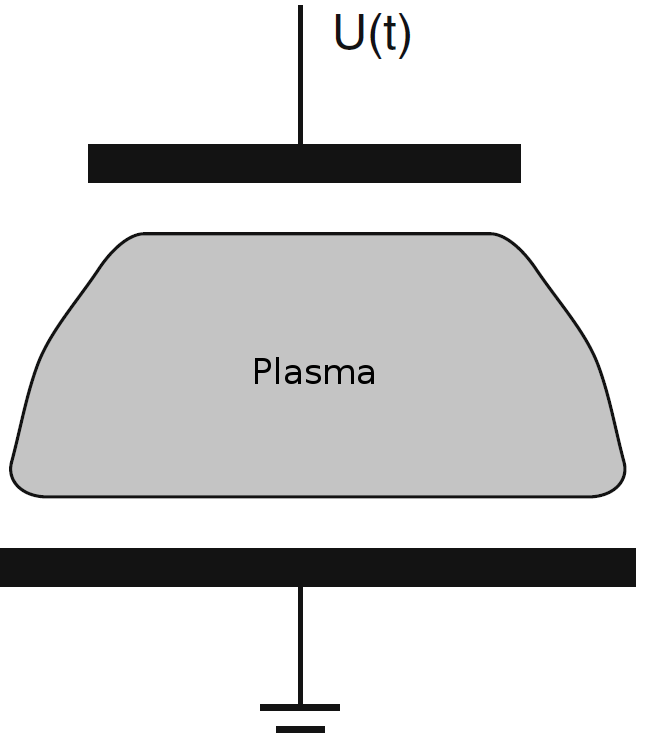
\includegraphics[width=0.7\textwidth,height=0.8\textwidth]{figs/schaltbildselfbiaspiel1.png}
								\caption{}
								\label{img:ungleichesplasma}
							\end{subfigure}
							\begin{subfigure}[b]{0.48\textwidth}
								\centering
								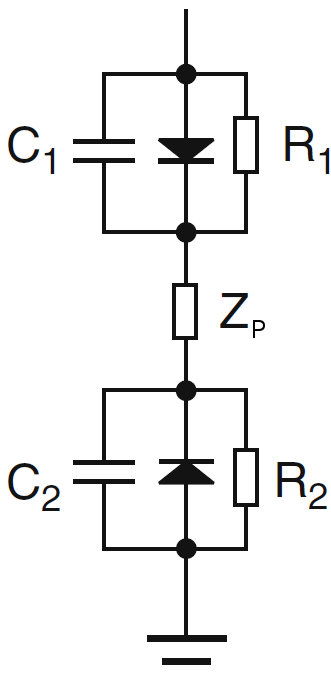
\includegraphics[width=0.4\textwidth,height=0.8\textwidth]{figs/schaltbildselfbiaspiel2.png}
								\caption{}
								\label{img:ersatzschaltbild}
							\end{subfigure}
							\caption{\fett{(a)}:Schema eines Plasmas mit ungleichen Elektrodenflächen. Die obere ist hierbei kleiner und gleichzeitig mit dem \tilt{rf}-Signal betrieben. \fett{(b)}:Ersatzschaltbild einer Entladung mit der \tilt{bulk}-Impedanz $Z\ix{P}$ (Hauptvolumen) und den Randschichten: eine Diode als Symbol für den "`Elektronenfluss"' aus der Schicht hinaus, der Widerstand $R\ix{j}$ als Ionenstrom und die Kapazität $C\ix{j}$ der pos. Raumladungszone (nach \cite{Piel10}).}
						\end{figure}

					Einem Plasma kann man eine, für \tilt{rf}-Spannungen der Frequenz $\omega$ nicht verschwindende Impedanz $Z\ix{P}$ zuordnen. Für das Entladungsvolumen der Permittivität $\varepsilon\ix{P}$, der Kapazität $C\ix{P}$ auf der Querschnittsfläche $A$ und Dicke $b$, in welcher die freien Elektronen mit der Frequenz $\nu\ix{e,N}$ mit den Neutralgasatomen stoßen, gilt (\cite{Piel10}):

					\begin{align}
					\varepsilon\ix{P}=1-&\frac{\omega\ix{P,e}^2}{\omega\left(\omega-\imag\nu\ix{e,N}\right)} \quad \quad C\ix{P}=\varepsilon\ix{P}C\ix{0}=\varepsilon\ix{P}\varepsilon\ix{0}\frac{A}{b} \\
					&Z\ix{P}=\left(\imag\omega C\ix{P}+ \frac{1}{\frac{1}{\omega\ix{P,e}^2C\ix{0}}\left(\nu\ix{e,N}+\imag\omega\right)}\right)^{-1}
					\label{eq:bulkimpedanz}
					\end{align}

					Die Induktivität $\imag\omega/\left(\omega\ix{P,e}^2C\ix{0}\right)$ des "`elektronisches Schaltkreises"' der Entladung gibt die Trägheit der Elektronen in Bezug auf ein Signal $\omega$ wieder, wohingegen der reele Widerstand $\nu\ix{e,N}/\left(\omega\ix{P,e}^2C\ix{0}\right)$ der Neutralgasreibung entspricht. Zusammen mit den Randschichten ergibt sich das Ersatzschaltbild eines Plasmas in \ref{img:ersatzschaltbild}.\\
					Betrachtet man zuerst den Fall hoher Anregungsfrequenzen, so kann man die Impedanz des \tilt{bulk} (siehe Gl. (\ref{eq:bulkimpedanz}), \cite{Kay85}) vernachlässigen und es dominieren die Kapazitäten $C\ix{j}$. Es folgt für die Spannung $U$ über die Entladung und das Plasmapotential $\Phi\ix{P}$:

						\begin{align}
							U\left(t\right)=U\ix{GS}+U\ix{rf}\sin\left(\omega t\right) \quad \quad \Phi\ix{P}\left(t\right)=\overline{\Phi\ix{P}}+\Phi\ix{rf}\sin\left(\omega t\right) \label{eq:selfbiaseins}
						\end{align}

					Wie bereits erwähnt, verschwindet die Randschicht vollständig während einer Anregungsperiode. Als Folge dessen stellt sich $\Phi\ix{P}$ auf das Potential der Elektrode ein, woraus wiederum ein Elektronenstrom auf diese folgt. Es entsteht sozusagen ein Kurzschluss in der Region der Randschicht, wenn das Plasmapotential negativ im Vergleich zur Elektrode wird. Es folgt somit mit Gl. (\ref{eq:selfbiaseins}) zusammen (nach \cite{Piel10}):

						\begin{align}
							\Phi\ix{P,max}=\overline{\Phi\ix{P}}+\Phi\ix{rf}\geq U\ix{Gs}+U\ix{rf} \quad \quad \Phi\ix{P,min}=\overline{\Phi\ix{P}}-\Phi\ix{rf}\geq 0\, \, . \label{eq:ungleichungen}
						\end{align}

					Liegt die getriebene Elektrode ohne zwischengeschalteten ``Puffer'' direkt an der \tilt{rf}-Signalquelle, so gilt zumindest f\"ur eine Ungleichung aus (\ref{eq:ungleichungen}) die Gleichheit. Wird hingegen die Elektrode kapazitiv gekoppelt, dh. zwischen diese und den Generator ein Kondensator geschaltet, so kann in einer Periode der \tilt{rf}-Anregung kein Nettostrom von der Quelle flie{\ss}en. Deswegen gibt es gleiche Elektronenstr\"ome auf beide Elektroden, was zur Folge hat, dass das minimale Plasmapotential das Massepotential wird und das maximale zu dem der Anregung. F\"ur den Gleichspannungsanteil, \tilt{self-bias} $U\ix{GS}$ und das mittlere Plasmapotential $\overline{\Phi\ix{P}}$ folgt:

						\begin{align}
							\overline{\Phi\ix{P}}=\frac{1}{2}\left(U\ix{GS}+U\ix{rf}\right) \quad \quad U\ix{GS}=\frac{C\ix{1}-C\ix{2}}{C\ix{1}+C\ix{2}}U\ix{rf} \,\, .\label{eq:selfbiaszwei} 
						\end{align}

					Diese Zusammenh\"ange gelten allgemein f\"ur dieses Experiment.\\
					Ist die Frequenz klein respektive \"ublicher Zeitskalen der Entladung, wie bspw. die Elektronen- oder Ionen-Plasmafrequenz (siehe \ref{tab:kenngroessen}), so wird der Strom aus den verdr\"angten Elektronen $j\ix{L}$ gr\"o{\ss}er als der Verschiebungsstrom durch die Randschichtschwankung $j\ix{V}\,$. Demzufolge wird der Strom aus Elektronen auf die getriebenen Elektrode, im Vergleich zu dem aus Ionen, durch einen Maxwell-Faktor in Abhängigkeit der angelegten Spannung verkleinert. Die Impedanz der Randschicht über der Elektrode ist demnach wesentlich größer als die der anderen bzw. der Wände. Mit den Gl. (\ref{eq:selfbiaseins}) und (\ref{eq:ungleichungen}) folgt, dass das Plasmapotential näherungsweise verschwindet und deswegen nur die Kontinuität für den Strom auf die getriebene Elektrode erhalten sein muss. Der \tilt{self-bias} bei kleinen Anregungsfrequenzen ergibt sich in Gl. (\ref{eq:selfbiasdrei}) ($\mathbf{J}\ix{0}$ \tilt{Bessel-Funktion}, nach \cite{Piel10}). 

						\begin{align}
							U\ix{GS}=\frac{k\ix{B}T\ix{e}}{e}\ln\left[\mathbf{J}\ix{0}\left(\frac{eU\ix{rf}}{k\ix{B}T\ix{e}}\right)\right] \label{eq:selfbiasdrei}
						\end{align}

					In \ref{img:imagundreal} ist der Spannungsverlauf beispielhaft dargestellt. Der \tilt{self-bias} verschwindet demnach nie für Elektrodenspannungen  $U\ix{rf}\neq0$ und ist damit eine feste Größe in einer Radiofrequenz-Entladung, welche über kapazitive Bauteile betrieben werden.

						\begin{figure}
							\centering
								\begin{subfigure}[t]{0.45\textwidth}
									\centering
									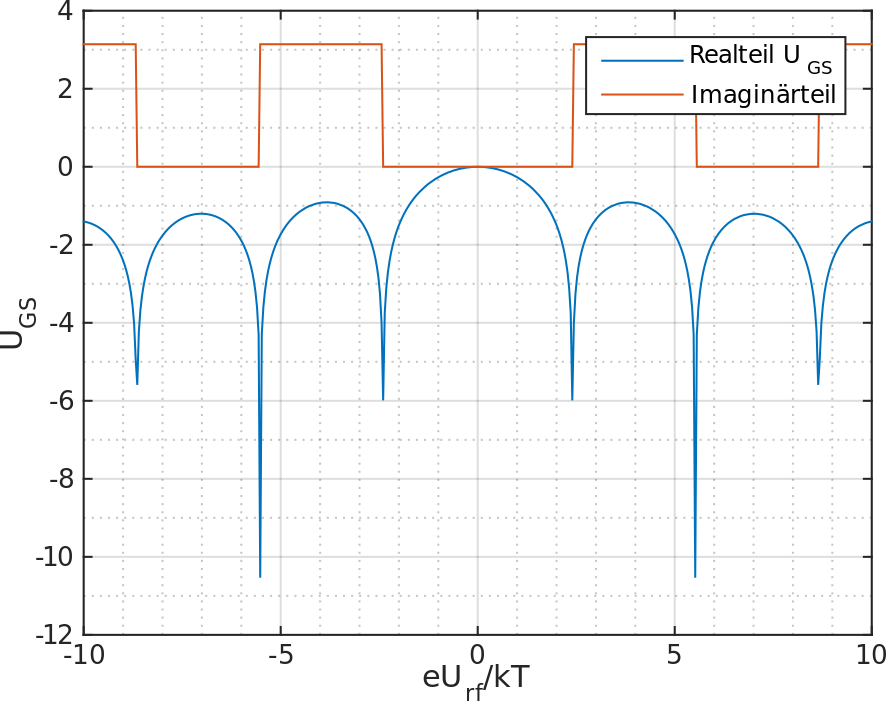
\includegraphics[width=\textwidth,height=0.8\textwidth]{figs/selfbiasselbst.png}
									\caption{}
									\label{img:imagundreal}
								\end{subfigure}
								\begin{subfigure}[t]{0.45\textwidth}
									\centering
									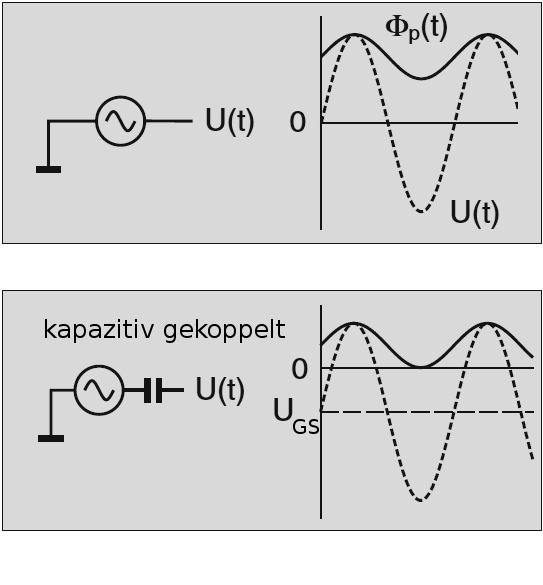
\includegraphics[width=0.7\textwidth,height=0.7\textwidth]{figs/kapazitivekopplungohneschemapiel.png}
									\vspace{-0.1cm}
									\caption{}
									\label{img:kapazitivgekoppelt}
								\end{subfigure}
								\caption{\fett{(a)}:Gleichspannungsanteil \tilt{self-bias} bei gegebenen Spannungen der Anregung $U\ix{rf}$, siehe Gl. (\ref{eq:selfbiasdrei}). \mbox{\fett{(b)}: Schema des} Potential- und Spannungsverlauf einer direkt und kapazitiv gekoppelten \tilt{rf}-Elektrode (nach \cite{Piel10}).}
						\end{figure}

		\subsection{Grenzschichten einer Entladung}\label{sub:rand}

			Im Hauptvolumen eines Plasmas werden die Neutralgasatome durch Wechselwirkungen mit den Elektronen zum Leuchten angeregt. Die Grenzschichten von Gasentladung sind jedoch dunkler, als das eigentliche Plasma. Dies ist auf einen Elektronenmangel zur\"uckruf\"uhren, ähnlich wie in Abschn. \ref{subsub:verschieb} argumentiert. Jedoch können auch Bereiche mit verschwindenden Elektronendichten hell leuchten, da der sog. \tilt{Glow} auch von der kinetischen Energie und Stoßeffizienz der Ladungsträger abhängt. Die Quasineutralit\"at kann in einer Randschicht demnach nicht mehr gelten. Es folgt, dass diese automatisch eine positive Raumladungszone ist. \\
			Auf Grund der wesentlich gr\"o{\ss}eren Beweglichtkeit $\upmu\ix{e}$ und thermischen Geschwindigkeit $v\ix{th,e}$, wird eine Wand in einem Plasma h\"aufiger von Elektronen getroffen, als von den korrespondierenden Ionen. Betrachtet man nur die Oberfl\"ache dieser, so kann man dessen Aufladung und damit auch das Potential $\Phi$ als negativ annehmen.

		\subsubsection{Child-Langmuir-Gesetz} \label{subsub:childlang}

		Die negative Aufladung einer Wand in einem Plasma soll nun eine große Potentialbarriere gegen thermische Elektronen erzeugen, e.g. $|\Phi\left(0\right)-\Phi\left(-d\right)|\ll k\ix{B}T\ix{e}/e\,$. Die Betrachtung in einer Dimension soll hier genügen - es lässt sich leicht der dreidimensionale Zusammenhang daraus erweitern. Die Elektronendichte $n\ix{e}\left(x\right)$ geht mit dem Boltzmann-Faktor $f\ix{B}\left(\Phi\right)$ ("`\tilt{boltzmann-artige}"' Elektronen) nach \cite{Piel10} wie

			\begin{align}
				n\ix{e}\left(x\right)=n\ix{e}\left(-d\right)f\ix{B}\left(\Phi\right)=n\ix{e}\left(-d\right)\exp\left(\frac{e\left(\Phi\left(x\right)-\Phi\left(-d\right)\right)}{k\ix{B}T\ix{e}}\right) \, . \label{eq:randschichtdichte}
			\end{align}

		Die Elektronendichte fällt damit exponentiell in Richtung der Wand ab. Das bedeutet, dass nur noch vorrangig Ionen ungehindert einströmen können. Es ist anzunehmen, dass die Randschichtausdehnung $d\ll\lambda\ix{mfp}$ die mittlere freie Weglänge des Plasma ist und die Ionen stoßfrei darin eintreten.\\
		An der Grenze zur Vorschicht (siehe \ref{img:dichterand}) haben die Ionen die Geschwindigkeit $v\ix{I,0}$ und das Potential der Wand verschwindet gerade an dieser Stelle. Für den Dichteverlauf der Ionen folgt:

			\begin{align}
				n\ix{I}\left(x\right)=n\ix{I}\left(-d\right)\left(1-\frac{2e\Phi\left(x\right)}{m\ix{I}v\ix{I,0}^2}\right)^{\frac{1}{2}}
			\end{align}

		Nimmt man weiterhin an, dass die kinetische Energie $m\ix{I}v\ix{I,0}^2/2\ll |e\Phi\left(x\right)|$ die Beschleunigung in der Randschicht ist, folgt somit die Bestimmungsgleichung (\ref{eq:potential}) für $\Phi\left(x\right)$ nach Poisson. Um dabei das korrekte Potential in der Grenzschicht zu erhalten, muss die Rückwirkung der Ionen auf dieses beachtet werden.

			\begin{align}
				\Delta\Phi\cong-\frac{en\ix{I}\left(-d\right)}{\varepsilon\ix{0}}\left(-\frac{2e\Phi\left(x\right)}{m\ix{I}v\ix{I,0}^2}\right)^{-\frac{1}{2}} \label{eq:potential}
			\end{align}

		Die klassische Lösung nach \tilt{Langmuir} für das eindimensionale $\Phi\left(x\right)$ erhält man aus Gl. (\ref{eq:potential}), wobei der ungestörte Ionenstrom geschrieben wurde als $j\ix{I}=n\ix{I}\left(-d\right)ev\ix{I,0}$.

			\begin{align}
				\Phi\left(x\right)=\left(\left(\frac{3}{4}\left(x+d\right)\right)^4\left(\frac{j\ix{I}}{\varepsilon\ix{0}}\right)^2\frac{m\ix{I}}{2e}\right)^{\frac{1}{3}}  \label{eq:langmuirpot}
			\end{align}

		Die Auflösung von Gl. (\ref{eq:langmuirpot}) nach dem Ionenstrom $j\ix{I}$ ergibt das \tilt{Child-Langmuir-Gesetz} ( Gl. (\ref{eq:childlang})). Dieses gibt nunmehr an, wie der Ionenstrom in der Randschicht von den Eigenschaften des ungestörten Plasmas abhängt. Umgekehrt bedeutet das, dass die Grenzregion auf Variationen des Potentials und der Parameter mit Veränderungen der Schichtdicke reagiert und damit versucht, den Einschränkungen der positiven Raumladungszone und dessen Ionenstrom nach dem \tilt{Child-Langmuir-Gesetz} zu genügen.

			\begin{align}
				j\ix{I}=\frac{4}{9}\varepsilon\ix{0}\left(\frac{2e\left(\Phi\left(-d\right)-\Phi\left(0\right)\right)^3}{m\ix{I}d^2}\right)^{\frac{1}{2}} \label{eq:childlang}
			\end{align}

				\begin{figure}
					\centering
					\begin{subfigure}[b]{0.6\textwidth}
						\centering
						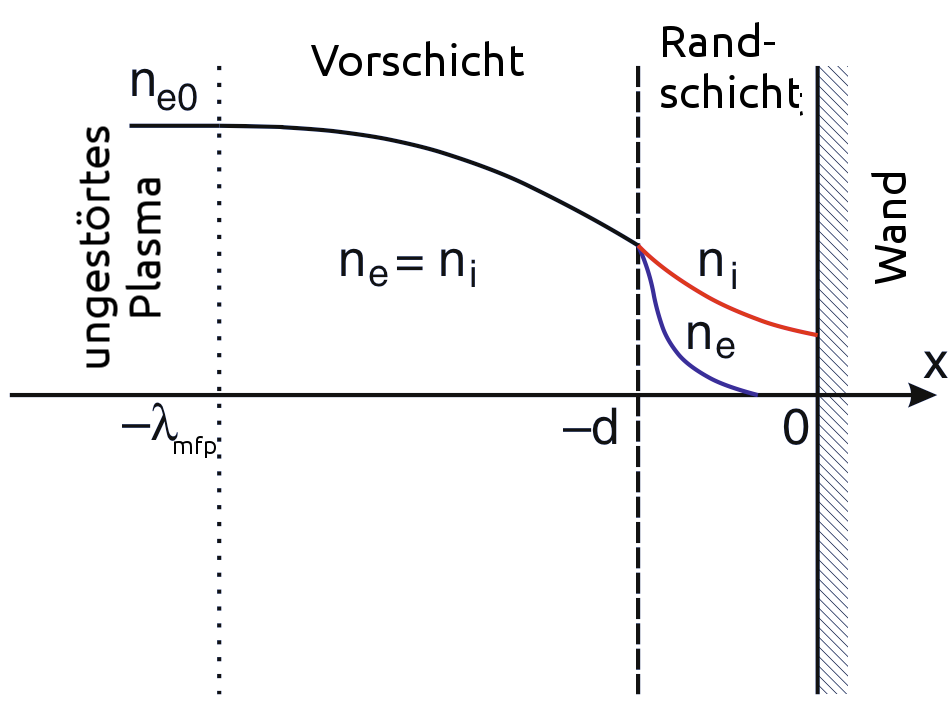
\includegraphics[width=0.7\textwidth,height=0.5\textwidth]{figs/randschichtpiel.png}
						\caption{}
						\label{img:dichterand}
					\end{subfigure}
					\begin{subfigure}[b]{0.375\textwidth}
						\centering
						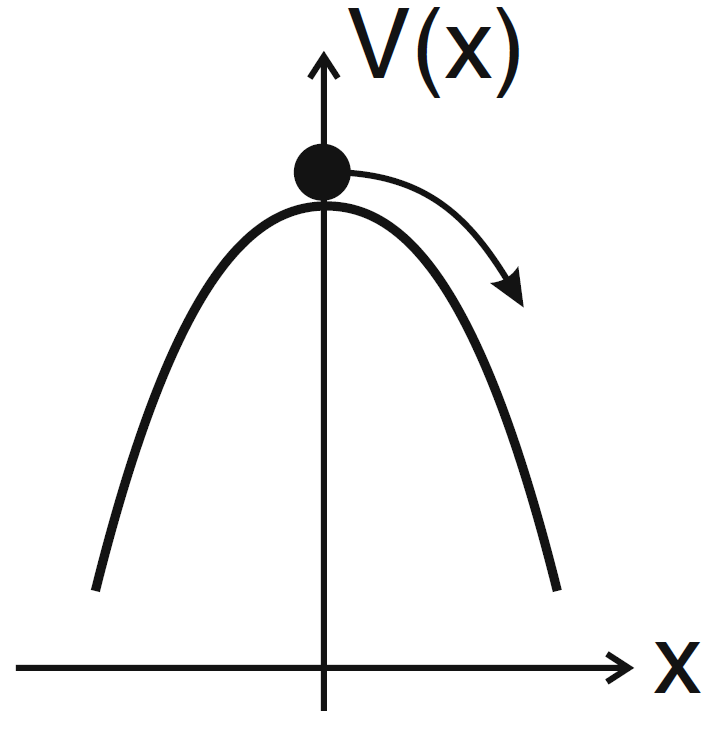
\includegraphics[width=0.8\textwidth,height=0.8\textwidth]{figs/parabelpiel.png}
						\caption{}
						\label{img:parab}
					\end{subfigure}
					\caption{\fett{(a)}: Dichten-Verlauf in der Grenzschicht zu einer Metalloberfläche. In einer bestimmten Entfernung $d$ zur Wand fällt die Elektronendichte praktisch auf 0, woraus die lokale Aufhebung der Quasineutralität folgt. \fett{(b)}: (Eindimensionales) Harmonisches Potential mit extremaler Instabilität. Kleine Auslenkungen sorgen für große Kräfte (nach \cite{Piel10}).}
				\end{figure}

		\subsubsection{Bohm-Kriterien}

			In Abschnitt (\ref{subsub:childlang}) wurde das Verhalten der Dichten der Ladungstr\"ager in einer Grenzschicht diskutiert. Diese erf\"ullen, in einem Abstand $d$ zur Wand in einem Plasma, die Eigenschaft der Quasineutralit\"at, welche weiterhin im Hauptvolumens gilt, nicht mehr. Es damit kein Kriterium f\"ur die Elektronen, welches sie daran hindert, auch aus weiten Teilen des Plasmas auf die Wand einzustr\"omen. Man stellt sich somit die Frage: Warum dehnt sich die Randschicht nicht in die gesamte Entladung aus? Wieso ist der Bereich der Elektronenersch\"opfung f\"ur eine Kombination der Plasmaparameter konstant? \\
			Um dieses Problem zu L\"osen, stellt man sich ein (mechanisches) Ein-Teilchen-Problem vor (\cite{Piel10}), bei welchem eine Gleichgewichtsanalyse vorgenommen wird. Das Potential habe ein Extremum - maximal oder minimal - an welchem die Punktmasse sich befindet. F\"ur den vorliegenden Fall des Randschicht-Problems sind nur Potentiale mit umgekehrt-parabelartigen Maxima interessant (siehe \ref{img:parab}), womit aus einer kleinen St\"orung eine gro{\ss}e Kraft auf das Teilchen folgt. In diesem Fall kann man also von einer Instabilit\"at sprechen.\\
			Der Bezug zur Plasmarandschicht wird deutlich, wenn man die Differentialgleichung des mechanischen Problems mit der Poissongleichung des Potentials in der Rand- bzw. Vorschicht - siehe Gl. (\ref{eq:pseudo}) vergleicht. Dabei stellt $\Psi\left(\Phi\right)$ ein Pseudopotential dar, welches in seiner Bedeutung vergleichbar mit der mechanischen Variante $V\left(\vec{r}\right)$ ist.

				\begin{align}
					m\frac{\diff^{2}\vec{r}}{\diff t^{2}}=-\frac{\diff V}{\diff\vec{r}} \quad \Leftrightarrow \quad \Delta_{\vec{r}}\,\Phi=-\frac{\diff\Psi}{\diff\Phi}=f\left(\Phi\right)\hspace{-0.3cm}\overset{Poisson}{\overset{\mid}{=}}\hspace{-0.3cm}\frac{\rho}{\varepsilon\ix{0}} \label{eq:pseudo}
				\end{align}

			Damit eine Instabilit\"at vorliegen kann, muss die, aus einer St\"orung des Pseudopotentials resultierende Kraft mit der Entfernung zum Gleichgewicht anwachsen. Die mathematisch \"aquivalente Formulierung ist die Ungleichung  in (\ref{eq:beding}). Nach Gl. (\ref{eq:pseudo}) und der in Abschnitt (\ref{subsub:childlang}) hergeleiteten Dichten in der Grenzschicht, kann die geforderte Bedingung \"uberpr\"uft werden. Aus ihr folgt das erste \tilt{Bohm-Kriterium}.

				\begin{align}
					0>\left.\frac{\diff^{2}\Psi}{\diff\Phi^{2}}\right|_{\Phi=0}\overset{Gl. (\ref{eq:pseudo})}{\overset{\mid}{=}}\left.\frac{\diff}{\diff\Phi}\left(\frac{n\ix{e}\left(x\right)-n\ix{I}\left(x\right)}{\varepsilon\ix{0}}\right)\right|_{\Phi=0}&=\frac{en\ix{e}\left(-d\right)}{\varepsilon\ix{0}}\left(\frac{e}{k\ix{b}T\ix{e}}-\frac{e}{m\ix{I}v\ix{0,I}^{2}}\right) \label{eq:beding} \\
					\Rightarrow \quad v\ix{0,I}\ge v\ix{B,I}=\sqrt{\frac{k\ix{B}T\ix{e}}{m\ix{I}}}& \label{eq:bohmkriteins}
				\end{align}

			($v\ix{B,I}$ - \tilt{Bohm}-Geschwindigkeit; $v\ix{0,I}$ - Ionen-Driftgeschwindigkeit; $T\ix{e}$ - Elektronentemperatur; $m\ix{I}$ - Ionenmasse)\\
			Für das Bohm-Kriterium in Gl. (\ref{eq:bohmkriteins}) kann auch analog die sog. \tilt{Machzahl} $M=v\ix{0,I}/v\ix{B,I}$ angegeben werden.\\
			Um zu erläutern, warum die Randschicht sich als Rückwirkung nicht in das Plasma ausdehnt, betrachten wir die Teilchenbewegung aus der Vor-Randschicht. Hier existiert ein elektrisches Feld, welches die Ionen auf die Geschwindigkeit $v\ix{B}$ in Richtung Wand beschleunigt. Außerdem gilt in ihr noch die Quasineutralitäts-Bedingung:

				\begin{align}
					n\ix{I}\left(x\right)=n\ix{I,0}\exp\left(\frac{e\Phi\left(x\right)}{k\ix{B}T\ix{e}}\right)=n\ix{e}\left(x\right)\,\, . \label{eq:bohmquasineutral}
				\end{align}

			Hierbei ist $\Phi\left(x\right)$ das Potential der Vorschicht aus Abschnitt  (\ref{subsub:childlang}). 
			Da Stöße der Frequenz $\nu\ix{N,I}$ der Ionen mit den Neutralgasatomen einen nicht vernachlässigbaren Einfluss auf deren Strom haben, muss die Geschwindigkeitsverteilung umgeschrieben werden.

				\begin{align}
					\frac{\diff v\ix{I}}{\diff x}=\frac{\nu\ix{N,I}v\ix{I}^2}{v\ix{B}^2-v\ix{I}^2} \label{eq:geschwindverteil}
				\end{align}

			Aus der Singularität von Gl. (\ref{eq:geschwindverteil}) in $v\ix{I}=v\ix{B}$ und der Kenntnis über das Wandpotential lässt sich die Ausdehnung der Randschicht $d$ bestimmen. Offensichtlich werden Ionen mit einer Geschwindigkeit $v\ix{I}<v\ix{B}$ in der Vorschicht beschleunigt. Geschwindigkeiten größer als die Bohm-Geschwindigkeit kommen dort nicht vor, da dies nach Gl (\ref{eq:bohmkriteins}) nur in der Randschicht der Fall sein darf. \\
			Zusammen mit dem ersten \tilt{Bohm-Kriterium} folgt, dass am Übergang der Vor- zur Randschicht die Ionen $v\ix{B}$ erreichen müssen, damit sich eine positive Raumladungszone ausbilden kann.

				\begin{align}
					M=1 \quad \Leftrightarrow \quad v\ix{I}\left(-d\right)=v\ix{B} \label{eq:bohmkritzwei}
				\end{align}

			Lokal heißt das, dass bei $x=-d$ die Dichten bereits auf $\approx0,66n\ix{e,0}$ abgefallen sind (siehe \ref{eq:bohmquasineutral}, \ref{img:dichterand}) und das Potential durch die Aufladung der Wand circa $-k\ix{B}T\ix{e}/2e$ beträgt.\\
			Ein Plasma "`sieht"' damit seine Randschicht nicht, da sich die notwendige Dynamik der entsprechenden Ladungsträger auf diese beschränkt und sich nicht beliebig ausdehnen kann. Mit anderen Worten: eine Randschicht bildet sich nur an Orten des Elektronenmangels und lokal negativer Potentiale aus.

		\subsection{Aufladung von Staubpartikeln}\label{sub:ströme}

			Die Ladung eines Fremdteilchens (Staub) in einem Plasma ist eine dynamische Größe. Sie ist sowohl zeitlich veränderlich, als auch abhängig von den Plasmaparametern, den Partikeleigenschaften sowie deren Trajektorie in der Entladung. Die Ladung eines Teilchens zum Zeitpunkt $t$ ergibt sich, näherungsweise, aus den Ladungsströmen $I\ix{k}$ der Plasmaspezies auf das Partikel bis zu diesem Zeitpunkt. Im folgenden genügt es, dieses Problem auf einer Zeitskala zu betrachten, in der man die Ladung als konstant unter dem Einfluss der Ströme annehmen kann. Damit werden diese ebenfalls stationär und es gilt für ein einzelnes Teilchens die \tilt{Kirchhoff'sche Knotenregel}, wobei der Staub ein Knoten sei:

				\begin{align}
					\sum_{\text{k}} I\ix{k}\left(\Phi\ix{fl}\right)=\frac{\diff Q\ix{S}}{\diff t} \,\, . \label{eq:float}
				\end{align}

		Die Elektronen und Ionen im Plasma strömen aufgrund ihrer thermischen Bewegung auf das Fremdteilchen und verleihen diesem über Stöße eine Ladung $Q\ix{S}$, wobei sich für das Partikel ein elektrostatisches Potential $\Phi\ix{fl}$, das sog. \tilt{floating} Potential, einstellt, für welches Gl. (\ref{eq:float}) gilt. Die Ladungsspezies können aus Sekundär-,Photo-, oder Feldemissionen kommen, wobei die dominanten Ströme die des Plasmas selbst sind. Hier soll es ausreichen, die Plasmaströme nach  \tilt{Langmuir} und \tilt{Mott-Smith} mit dem sog. \tilt{orbital motion limit}-Modell \cite{Langmuir26} zu beschreiben. 

			\subsubsection{OML-Modell}\label{subsub:oml}

						\begin{figure}
							\centering
							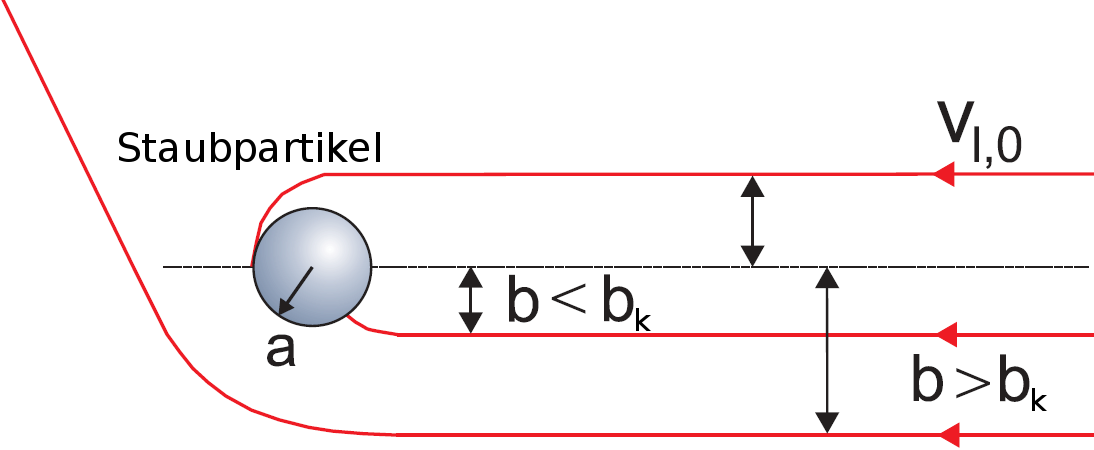
\includegraphics[width=0.7\textwidth, height=0.3\textwidth]{figs/orbitalmotionlimitmelzer.png}
							\caption{OML-Beschreibung eines, auf ein Staubpartikel einströmendes Ions. Der kritische Stoßparameter, für welcher eine Kollision stattfindet, ist $b\ix{k}$. Er ist im Vergleich zum geometrischen Querschnitt aufgrund der Coulomb-Wechselwirkung vergrößert (nach \cite{Melzer12}).}
							\label{img:oml}
						\end{figure}

			Dabei wird angenommen, dass sich ein strömendes Teilchen, welches zu $Q\ix{S}$ beiträgt bzw. damit elektrostatisch wechselwirkt, stoßlos aus dem Unendlichen (durch die Entladung) darauf zu bewegen kann. Aufgrund der, im allgemeinen höheren Elektronentemperatur und -beweglichkeit wird $\Phi\ix{fl}<0$, woraus eine veränderte Wechselwirkung mit den Teilchen der Ladungsströme folgt. Man definiert folglich einen kritischen Stoßparameter $b\ix{k}$, welcher dem Abstand eines Ions zur Target-Achse entspricht, bei dem dieses durch die Coulomb-Anziehung des Partikels gerade noch dessen Oberfläche tangiert. Für Parameter $b>b\ix{k}$ wird ein eintreffendes Ion auf seiner Trajektorie nur abgelenkt, für $b<b\ix{k}$ landet dieses auf dem Staubteilchen, siehe \ref{img:oml}.\\
			Da vorausgesetzt wurde, dass keine Stöße vor dem Target geschehen, kann die Impulserhaltung zusammen mit der Energieerhaltung für ein einzelnes Projektil aufgestellt werden, welches sich im Abstand $b\ix{k}$ darauf zu bewegt (hier aus \cite{Melzer12}):

				\begin{align}
					|\vec{L}|=|\vec{r}\times\vec{p}|=m\ix{I}v\ix{I}a=m\ix{i}v\ix{i,0}b\ix{k} \label{eq:impulserhaltung} \\
					E\ix{I}=\frac{m\ix{I}}{2}v\ix{I}^2+e\Phi\ix{fl}=\frac{m\ix{I}}{2}v\ix{I,0}^2 \label{eq:energieerhaltung}
				\end{align}

			In Gl.(\ref{eq:impulserhaltung}) und (\ref{eq:energieerhaltung}) stehen jeweils die linken Seiten für den Zeitpunkt des Auftreffens und die rechten für das Einlaufen aus dem Unendlichen. Durch Umformungen lässt sich ein Ausdruck für den kritischen Stoßparameter, in Abhängigkeit vom Partikelradius und dem \tilt{floating}-Potential aufgestellt werden.

				\begin{align}
					b\ix{k}^2=a^2\left(1-\frac{e\Phi\ix{fl}}{\frac{m\ix{I}}{2}v\ix{I,0}^2}\right) \label{eq:krit}
				\end{align}

			Der zugehörige Streuquerschnitt für die Streuung eines Teilchenstroms an einem Staubpartikel wird damit zu $\sigma\ix{k}=\pi b\ix{k}^2$, welcher größer als die geometrische Querschnittsfläche $\pi a^2$ ist. Dem liegt die Coulomb-Wechselwirkung der Stoßpartner zu Grunde.\\
			Der (differentielle) Ladungsträgerstrom $\diff I\ix{j}$, welcher schließlich den Parameter der Partikelladung bestimmt, ergibt sich aus der Aufsummierung aller Stromdichten von Teilchen der Geschwindigkeiten $v\ix{j}$, gewichtet mit ihren zugehörigen Wechselwirkungsquerschnitten $\sigma\ix{j}$ und (hier: maxwellartigen) Verteilungen $f\left(v\ix{j}\right)$ (\cite{Melzer12}):

				\begin{align}
					\diff I\ix{j}=\sigma\ix{j}&\left(v\ix{j}\right)n\ix{j}v\ix{j}f\left(v\ix{j}\right)\diff v\ix{j} \nonumber \\
					\text{Ionen: } I\ix{I}&=\pi a^2n\ix{I}e\sqrt{\frac{8k\ix{B}T\ix{I}}{\pi m\ix{I}}}\left(1-\frac{e\Phi\ix{P}}{k\ix{B}T\ix{I}}\right) \label{eq:ionenstrom} \\
					\text{Elektronen: } I\ix{e}&=-\pi a^2n\ix{e}e\sqrt{\frac{8k\ix{B}T\ix{e}}{\pi m\ix{e}}}\exp\left(\frac{e\Phi\ix{P}}{k\ix{B}T\ix{e}}\right) \label{eq:elektronenstrom}
				\end{align}

			($T\ix{e,I}$ - Elektronen-/Ionentemperatur; $n\ix{e,I}$ - Elektronen-/Ionendichte, $\Phi\ix{P}$ - Partikelpotential; $k\ix{B}$ - \tilt{Boltzmann}-Konstante )\\
			Der Unterschied zwischen Gl. (\ref{eq:ionenstrom}) und (\ref{eq:elektronenstrom}) resultiert aus den unterschiedlichen Arten der Wechselwirkung mit dem Staubteilchen. Da $\Phi\ix{P}<0$ ist, werden Ionen aller Geschwindigkeiten in Richtung des Partikels gelenkt und könnten theoretisch damit stoßen (mit Rücksicht auf die Geschwindigkeitsverteilung und den Streuquerschnitt). Die Elektronen hingegen müssen mindestens eine Geschwindigkeit $v\ix{min}=\sqrt{-2e\Phi\ix{P}/m\ix{e}}$ besitzen, damit sie die Potentialbarriere zum Partikel überwinden und damit stoßen können. Au{\ss}erdem finden sich mit $\sqrt{8k\ix{B}T\ix{j}/\pi m\ix{j}}$ die thermischen Geschwindigkeiten der jeweiligen Spezies $j$ als Vorfaktoren wieder. Damit werden die Gesamtstr\"ome letztendlich zum Produkt aus ungest\"orter, thermischer Stromdichte und der angepassten Wechselwirkungsfl\"ache des Partikels. \\
			Es sei erwähnt, dass aufgrund der hohen Teilchendichten in einem Plasma die OML-Theorie nicht der Realität entspricht. Die mittlere freie Weglänge eines Ions oder Elektrons hat in etwa die Dimension der Debyelänge $\lambda\ix{D}$ und ist nicht, wie vorausgesetzt, unendlich groß. Des weiteren entsprechen die $f\left(v\ix{j}\right)$ in der Praxis nicht isotropen Maxwell-Geschwindigkeitsverteilungen.

			\subsubsection{Neutralgas-Ionen-Stöße}

			Auf Grundlage der OML-Theorie lässt sich ein erweiterter Ausdruck für den Ionenstrom mit Rücksicht auf Stöße des Neutralgases aufstellen. Offensichtlich geht, mit dem Durchgang eines Projektils durch das Neutralgas einer Entladung, der Verlust kinetischer Energie einher. Es ist nun leicht nachzuvollziehen, dass sich Ionen, aufgrund der Ablenkungen durch Stöße und Wechselwirkung, um das negativ geladene Staubpartikel sammeln (\cite{Goree92}).\\
            In einer Sphäre mit dem Radius $R$ um das Teilchen ist die Stoßwahrscheinlichkeit zwischen Ionen und Neutralgasatomen

				\begin{align}
					\frac{R}{l\lambda\ix{mfp}}=Rn\ix{N}\sigma\ix{I,N} \,\, . \label{eq:wahrschein}
				\end{align}

			($n\ix{N}$ - Neutralgasdichte; $\sigma\ix{I,N}$ - Stoßparameter für Ion-Neutralgas-Stöße; \mbox{$\lambda\ix{mfp}$ - mittlere freie Wegl\"ange})\\
			Durch eine Sph\"are mit diesem Radius flie{\ss}t nun neben dem thermischen Ionenstrom $I\ix{th}$ noch ein weiterer Strom $I\ix{S}$ auf Grund der St\"o{\ss}e mit dem Neutralgas. Die Ionen der Geschwindigkeit $v\ix{th,I}$, welche sich ohne Wechselwirkung mit dem Gas der Entladung am Target vorbei bewegen w\"urden, werden mit der Sto{\ss}wahrscheinlichkeit aus Gl. (\ref{eq:wahrschein}) in Richtung des Staubteilchens abgelenkt und tragen somit zum Ladungsstrom auf dieses bei. Der Gesamtladungsstrom durch Ionen entspricht nach \cite{Lampe01} der Summe der beiden Str\"ome:

				\begin{align}
					I\ix{th}=&\pi R^{2}n\ix{N}ev\ix{th,I} \quad I\ix{S}=\pi R^2n\ix{N}ev\ix{th,I}\left(Rn\ix{N}\sigma\ix{N,I}\right) \\
					&I\ix{ges}=\pi a^{2}n\ix{I}ev\ix{th,I}\left(1-\frac{e\Phi\ix{P}}{k\ix{B}T\ix{I}}+\frac{R^{3}}{\lambda\ix{mfp}a^{3}}\right)
				\end{align}

			Auf der Oberfl\"ache der '\tilt{Sto{\ss}sph\"are}' $\mathbb{S}\ix{R}$ hat das \tilt{Yukawa}-Potential des Staubteilchens gerade die Energie der thermischen Ionenbewegung (Gl. (\ref{eq:bestimmR})), womit diese gerade noch in dessen Einfang geraten. Mit dem daraus bestimmten $R$ folgt nach (\cite{Melzer12},\cite{Khrapak05a}) ein diskreter Ionenstrom auf das Partikel mit R\"ucksicht auf die Ionen-Neutralgaswechselwirkung (Gl. (\ref{eq:ionstromkorr})).

				\begin{align}
					\frac{k\ix{B}T\ix{I}}{e}=&\frac{Z\ix{S}e}{4\pi\varepsilon\ix{0}R}\exp\left(\frac{R}{\lambda\ix{D}}\right) \label{eq:bestimmR} \\
					I\ix{I}=\pi a^{2} n\ix{I}e v\ix{th,I}&\left(1-\frac{e\Phi\ix{P}}{k\ix{B}T\ix{I}}+0,1\left(\frac{e\Phi\ix{P}}{k\ix{B}T\ix{I}}\right)^{2}\frac{\lambda\ix{D}}{\lambda\ix{mfp}}\right) \label{eq:ionstromkorr}
				\end{align}

			Im Vergleich zum Ergebnis des OML-Modells aus Gl. (\ref{eq:ionenstrom}) ist dieser Ladungstrom in Abh\"angikeit des Partikelpotentials und Ionentemperatur vergr\"o{\ss}ert. Die Wechselwirkung mit dem Neutralgas sorgt also, \"uber die St\"o{\ss}e und Erzeugung einer \tilt{Ionenwolke} um ein Teilchen, f\"ur einen gr\"o{\ss}eren pos. Ladungsstrom, welcher respektive wiederum f\"ur eine Steigerung des Elektronenstromes auf Grund des ver\"anderten Partikelpotentials sorgt. Eine selbstkonsistente L\"osung der, an den Anfang gestellte Problematik in Gl. (\ref{eq:float}) um das \tilt{floating}-Potential gestaltet sich jedoch als \"uberaus schwierig, da schon der OML-Theorie mehrere falsche Annahmen vorausgingen und dessen Eigenr\"uckwirkungen nicht-trivial sind.\\
			Um abschließend die Staubladung zu bestimmen, kann man das Modell eines Kugelkondensators hernehmen und dieses mit einer Abschirmung $a/\lambda\ix{D}$ verknüpfen (nach \cite{Melzer12}).

				\begin{align}
					Q\ix{S}=Z\ix{S}e=C\ix{S}\Phi\ix{fl}=4\pi\varepsilon\ix{0}a\left(1+\frac{a}{\lambda\ix{D}}\right)\Phi\ix{fl} \label{eq:ladung}
				\end{align}

			Für typische Laborplasmen kann das \tilt{floating}-Potential zu $\Phi\ix{fl}\approx-2k\ix{B}T\ix{e}/e$ genähert werden, woraus die Ladungszahl sich zu $Z\ix{S}\approx1400\cdot a/\unit[1]{\upmu m}\cdot T\ix{e}/\unit[1]{eV}$ ergibt.

		\subsection{Staub-Dynamik}\label{sub:dynamik}

			In einem Plasma wirken viele, u.U. nicht-triviale Kräfte auf den eingefangenen Staub. Im Folgenden werden die wichtigsten Einflüsse und Kenngrößen der Dynamik komplexer Plasmen vorgestellt und beschrieben (nach \cite{Melzer10}). Insbesondere ist dieser Abschnitt wichtig für das Verständnis über die Bildung und Stabilität sog. \tilt{Yukawa-Cluster}. Dabei handelt es sich um ein System aus wenigen Staubteilchen, welche sich in einem äußeren, harmonischen Potential auf konzentrischen Kugelschalen anordnen. Diese sollen des Weiteren genauer in Abschnitt \ref{sub:yukawaclust} beschrieben werden.

			\subsubsection{Gravitation und elektrische Feldstärke}\label{subsub:grav}

			Betrachtet man ein Experiment, welches am Erdboden durchgeführt wird, so muss die vollständige Gravitationskraft berücksichtigt werden. Dies gilt beispielsweise nicht für Versuche unter Mikrogravitation während Parabelflügen oder auf der \tilt{International Space Station}.

				\begin{align}
					F\ix{g}=m\ix{S} g=\frac{4}{3}\pi a^3 \rho\ix{S} g
				\end{align}

			($m\ix{S}$ - Masse der Staubteilchen; $a$ - Partikelradius; $\rho\ix{S}$ - Massendichte des Staubes; $g$ - \mbox{Erdbeschleunigung})\\
			Natürlich wirkt auf die, durch das ionisierte Gas elektrisch geladenen Partikel eine elektrische Kraft $F\ix{E}$, welche aus dem äußeren Feld $E$ der \tilt{rf}-Elektroden folgt. Eine elektrische Wechselwirkung mit dem Plasma tritt aufgrund der Quasineutralität nicht auf: innerhalb einer \tilt{Debye-Kugel} sind die Veränderung zu schnell, als dass das träge Staubteilchen diesen folgen könnte. 

				\begin{align}
				F\ix{E}=Q\ix{S} E=4 \pi \varepsilon\ix{0} a \Phi\ix{fl} E
				\end{align}

			($Q\ix{S}$ - Staubladung; $\Phi\ix{fl}$ - \tilt{floating}-Potential)\\
			Diese beiden Kräfte heben sich gerade in der Randschicht einer Radiofrequenz-Entladung auf, da sie antiparallel zueinander stehen. Zu beachten ist hierbei der stark unterschiedliche Einfluss des Teilchenradius - $F\ix{g}\propto a^3$ und $F\ix{E}\propto a$.\\

			\subsubsection{Abschirmung und Polarisationskräfte}\label{subsub:abschirm}

			Die große negative Aufladung der Staubteilchen sorgt über die Coulomb-Wechselwirkung mit den auf das Partikel zuströmenden Ionen dafür, das sich die Konzentration derer lokal stark ändert. Es entsteht eine Wolke aus langsamen Ionen die quasi in der näheren Umgebung um das Teilchen verbleiben, jedoch nicht mit diesem interagiert und es nach außen hin vor dem Einfall schnellerer pos. Ladungen abschirmen. Somit gibt es keine direkte Rückwirkung der Wolke auf das Partikel, sofern dessen sphärische Symmetrie gegeben ist. Gilt dies nicht, so entsteht ein Multipol- bzw. Dipolmoment $\vec{p}$, welches danach strebt, sich in Richtung des Feldes $\vec{E}$ auszurichten. Damit wirkt eine Kraft $F\ix{Dip}$ (für ein Dipolmoment) auf das Staubteilchen zurück, welche mit dem Gradienten der Richtungsdifferenz zwischen $\vec{p}$ und $\vec{E}$ geht.

				\begin{align}
					\centering
					\vec{F}\ix{Dip}&=\vec{\nabla}\left(\vec{p}\vec{E}\right)\\
					&{\overset{\vec{p}\,||\vec{E}}{=}}\grad{pE} \nonumber
				\end{align}

			Das besagte Dipolmoment entsteht u.a. durch die diversen, gerichteten Ladungsprozesse in dem Plasma. Ein Partikel, welches in der Randschicht eingefangen und von einer Ionenwolke umgeben wird, 'sieht' unterschiedliche \tilt{Debye}-Längen über und unter sich aufgrund der lokalen Feldrichtung und der stark vom Mittelwert abweichenden Ionen- und Elektronendichten. Somit ändert sich offensichtlich die Plasmadichte innerhalb des Volumens einer Kugel mit dem, nun ortsabhängigen Radius $\lambda\ix{D}\left(\vec{r}\right)$. Insgesamt folgt daraus eine neue Bestimmungsgleichung für das Potential und damit auch eine neue Kraft $F\ix{E}$.

				\begin{align}
					\Delta \Phi\left(\vec{r}\right)-\frac{\Phi\left(\vec{r}\right)}{\lambda\ix{D}^2\left(\vec{r}\right)}=\frac{Q\ix{s}}{\varepsilon\ix{0}}\delta\left(\vec{r}\right) \\
					F\ix{E}=\underbrace{Q\ix{S}E}_{\text{(I)}}-\underbrace{\frac{Q\ix{S}^2}{8\pi\varepsilon\ix{0}}\frac{\nabla\lambda\ix{D}\left(\vec{r}\right)}{\lambda\ix{D}^2}}_{\text{(II)}}
				\end{align}

			Hierbei stellt (I) die normale Komponente dar und (II) ist zusätzliche Kraft durch die Deformation der Ionenwolke in Richtung kleinerer \tilt{Debye}-Längen $\lambda\ix{D}\left(\vec{r}\right)$. Die Kraft $F\ix{E}$ kann also dadurch größer oder kleiner werden. Hinzu kommt, dass der veränderte Parameter $\lambda\ix{D}$ von der Driftgeschwindigkeit $u\ix{I}$ abhängt, welche die Ionenwolke maßgeblich beeinflusst. Ist jedoch $u\ix{I}<v\ix{th,I}$ so kann man annehmen, dass die Ionenwolke besteht und $\lambda\ix{D}\left(\vec{r}\right)\approx\lambda\ix{D,I}$ gilt.\\
			Sind die Ionen jedoch schneller, womit $u\ix{I}>>v\ix{th,I}$ wird, so können sie nicht mehr vom Feld des Partikels 'gefangen' werden und damit die Ionenwolke bilden. So gilt folglich $\lambda\ix{D}\left(\vec{r}\right)\approx\lambda\ix{D,e}$.\\
			Insgesamt ist der Einfluss der Polarisation vernachlässigbar klein, solange die Teilchen eine Größe von einigen hundert $\unit{\upmu m}$ nicht übersteigen.

		\subsubsection{Ionen-Reibung}\label{subsub:reibung}

			Aufgrund der hohen negativen Ladung des Staubteilchens und der daraus resultierenden elektrostatischen Wechselwirkung existiert ein, relativ auf das Partikel zufließender, Ionenstrom oder auch "`Ionenwind"'. Weiterhin bewegen sich Neutralgasatome durch das Plasma und stoßen mit anderen Teilchen. Die Zahl der Stöße $\diff N$ einer Spezies mit einem Target mit dem Streuparameter $\sigma$ im Zeitintervall $\diff t$ ist somit über deren relative Geschwindigkeit $v\ix{rel}$ zu diesem in $\diff N=n\sigma v\ix{rel}\diff t$ gegeben. Hierbei kennzeichnet $n$ die Stromdichte der strömenden Teilchen. Aus diesem Strom folgt ein gewisser Impulsübertrag $\Delta p$ auf das Target. Hieraus lässt sich eine Kraft $F\ix{drag}$ ziehen, die einer Reibung bzw. einer Impulsaufnahme entspricht.

				\begin{align}
					F\ix{drag}=\frac{\diff N \Delta p}{\diff t}=\Delta p n \sigma v\ix{rel}
				\end{align}

			 Man kann diese aus 2 Teilen aufbauen: direkte Kollisionen mit den Ionen $F\ix{dir}$ und deren Coulomb-Streuung an den Feldern der neg. geladenen Staubpartikel. Im folgenden soll das sog. \tilt{Barnes-Modell} eingeführt werden, welches die besagte Ionenreibung beschreibt.

				\paragraph{Ionenreibung: \tilt{Barnes-Modell}}

				Für die Bestimmung von $F\ix{dir}$ wird angenommen, dass nur die Ionen, welche für eine Ladungsänderung der Partikel sorgen, auch diese direkt treffen. Im Rückblick auf die Bestimmung der Ionenströme in \ref{sub:ströme} wird die Kraft durch Kollisionen zu

					\begin{align}
						F\ix{dir}=\pi a^2m\ix{I}\tilde{v}n\ix{I}u\ix{I}\left(1-\frac{2e\Phi\ix{fl}}{m\ix{I}\tilde{v}^2}\right)\,\,.
					\end{align}

				($n\ix{I}$ - Ionenkonzentration; $u\ix{I}$ - Ionen-Driftgeschwindigkeit; $m\ix{I}$ - Ionenmasse)\\
				Das Produkt aus Masse und mittlerer Geschwindigkeit der Ionen $m\ix{I}\tilde{v}=m\ix{I}\sqrt{u\ix{I}^2+v\ix{th,I}^2}$ entspricht dem Impulsübertrag.\\
				Für die Coulomb-Streuung müssen alle diejenigen Ionen miteinbezogen werden, welche mit dem Feld des Staubes 'stoßen'. Hierfür wird der Streuquerschnitt $\tilde{\sigma}$ nach \cite{Barnes92} der Ionen-Elektronen-Wechselwirkung auf den aktuellen Fall angepasst.

					\begin{align}
						\tilde{\sigma}=4\pi b_{\frac{\pi}{2}}^2\ln\left(\Lambda\right)=&\,4\pi b_{\frac{\pi}{2}}^2\ln\left(\frac{\lambda\ix{D}}{b_{\frac{\pi}{2}}}\right) \\
						\text{wobei }\, b_{\frac{\pi}{2}}=&\,\frac{e^2}{4\pi\varepsilon\ix{0}m\ix{I}v^2} \nonumber
					\end{align}

				Der Stoßparameter $b_{\frac{\pi}{2}}$ beschreibt eine Ablenkung um $\unit[90]{\degree}$. Für die Ionenreibung müssen weitere Bedingungen mit eingebunden werden: die Coulomb-Streuung außerhalb der Ionenwolke ist irrelevant, die Staubpartikel haben eine endliche Ausdehnung und damit existiert ein minimaler Stoßparameter $b\ix{k}$. Damit wird das gesuchte $\sigma$ zu

					\begin{align}
						\sigma=\int_{b\ix{k}}^{\lambda\ix{D}}\tilde{\sigma}\diff\left(\frac{\lambda\ix{D}}{b_{\frac{\pi}{2}}}\right)=&\,4\pi b_{\frac{\pi}{2}}^2\ln\left(\frac{\lambda\ix{D}^2+b_{\frac{\pi}{2}}^2}{b\ix{k}^2+b_{\frac{\pi}{2}}^2}\right)^{1/2} \nonumber \\
						F\ix{Coul}\overset{(*)}{=}&\,\frac{2\pi a^2 e^2\Phi\ix{fl}^2}{m\ix{I}\tilde{v}^3}n\ix{I}u\ix{I}\ln\left(\frac{\lambda\ix{D}^2+b_{\frac{\pi}{2}}^2}{b\ix{k}^2+b_{\frac{\pi}{2}}^2}\right)^{1/2} \, \, .
					\end{align}

				Den $\ln\left(\dots\right)$ nennt man auch den \tilt{Coulomb-Logarithmus} $\ln\left(\Lambda\right)$.\\
				In (*) wurde für die vollständige Coulomb-Kraft durch Ionen $F\ix{Coul}$ auf ein Partikel benutzt, dass dieses mit Ladung $Z\ix{S}e=Q\ix{S}$ als Kugelkondensator mit $Q\ix{S}=4\pi\varepsilon\ix{0}a\Phi\ix{fl}$ ausgedrückt werden kann. Wichtig zu beachten ist jedoch, dass nur Ionen einen Beitrag leisten, die innerhalb eines Stoßparameters $\lambda\ix{D}\approx\lambda\ix{D,e}$ (nach \cite{Kilgore93}) am \tilt{target} vorbei fliegen.\\
				Die gesamte Kraft durch Ionen auf die Staubteilchen ist somit die Summe der Kräfte aus direkten Stößen und Coulomb-Kollisionen $F\ix{ion}=F\ix{dir}+F\ix{Coul}$, welche zusammen dargestellt sind in \ref{img:ionkräfte}.

					\begin{figure}
						\centering
						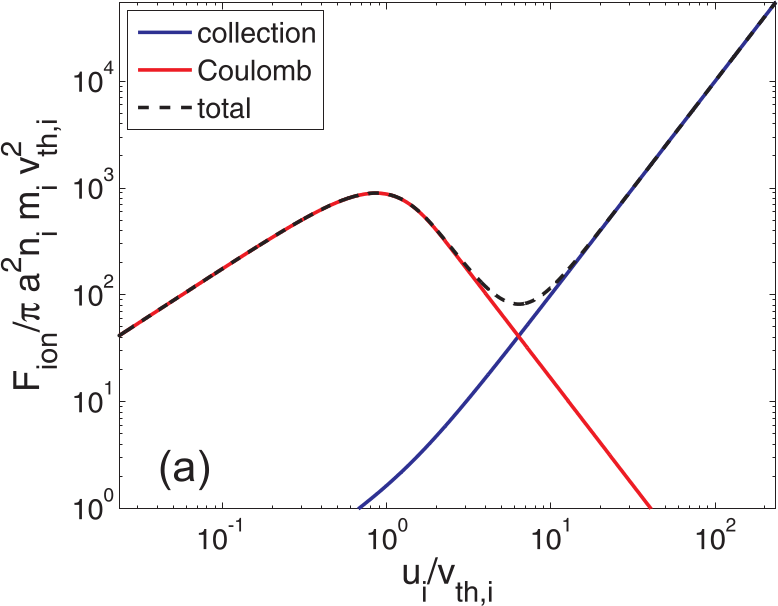
\includegraphics[height=0.4\textwidth,width=0.6\textwidth]{figs/forcesandtrappingmelzer.png}
						\caption{Berechnete Kräfte $F\ix{Coul}$ (\tilt{Coulomb}), $F\ix{dir}$ (\tilt{collection}) und die Summe beider auf einer doppelt-logarithmischen Skala(nach \cite{Melzer12}).}
						\label{img:ionkräfte}
					\end{figure}

		\subsubsection{Neutralgasreibung}

			Die Stöße mit den Neutralgasatomen können, ebenso wie die mit Ionen, als Kraft durch Reibung aufgefasst werden. Diese sorgen insbesondere für eine Verlangsamung der Bewegung der Staubteilchen. Die Kraft $F\ix{N}$ wird, in ähnlicher Weise wie $F\ix{dir}$, durch einen Impulsübertrag über einen Strom von Neutralgasteilchen auf einen effektiven Querschnitt ausgedrückt (\cite{Epstein24}).

				\begin{align}
					F\ix{N}=-\delta\frac{4}{3}\pi a^3m\ix{N}v\ix{th,N}n\ix{N}v\ix{S}
				\end{align}

			($m\ix{N}$ - Neutralgasatommasse; $v\ix{th,N}$ - thermische Geschw. der Neutralgasatome; $n\ix{N}$ - Neutralgasdichte; $v\ix{S}$ - Staubteilchengeschw.)\\
			Der Faktor $\delta$ beschreibt hierbei die Art, wie die Neutralgasatome mit dem Staub stoßen. Eine spiegelnde Reflexion tritt für ein $\delta=1$ auf. Mit steigendem $\delta$ wird die Kollision immer diffuser, bis hin zu einem Wert von $\delta=1,44$.\\
			Für den berühmten \tilt{Milikan}-Öltropfen-Versuch zur Bestimmung der Ladung eines Elektrons wurde, 1924 von \tilt{P. S. Epstein}, ebenso ein Ausdruck für die Kraft durch Neutralgasreibung bestimmt. Dabei ist $\beta$ der Reibungskoeffiziént und $\rho\ix{S}$ die Dichte des Staubmediums.

				\begin{align}
					F\ix{N}=-m\ix{S}\beta v\ix{S}=-m\ix{S}v\ix{S}\delta\frac{8}{\pi}\frac{p}{a\rho\ix{S}v\ix{th,N}}
				\end{align}

		\subsubsection{Thermophoretische Kraft}\label{subsub:therm}

			In einer Plasmakammer kann, durch Aufheizung oder Abkühlung einer der Elektroden bzw. Kammerbegrenzungen ein, der Gravitation oder dem elektrischen Feld entgegen gerichteter Temperaturgradient angelegt werden.\\
			Die Kraft kann folgendermaßen erklärt werden: auf der Seite der höheren Temperatur haben die Neutralgasteilchen im Mittel eine größere Geschwindigkeit und Impuls, woraus ein positiver Impulsübertrag in Richtung niedrigerer Temperaturen folgt.	Mit der Wärmeleitfähigkeit des Neutralgases $\kappa\ix{N}$ folgt für die thermophoretische Kraft $F\ix{th}$ Gl. (\ref{eq:therm}). Auf Grund $\propto a^2$ ist diese Kraft besonders wichtig für Teilchen mit einem Radius kleiner als $\unit{\upmu m}$. Sie wird für die Formation von sog. \tilt{Yukawa-Clustern} (siehe \ref{sub:yukawaclust}) oder zur Herstellung von "`Quasi-Schwerlosigkeit"' (siehe \cite{Rothermel02}) genutzt.

				\begin{align}
					F\ix{th}=-\frac{32}{15}\frac{a^2 \kappa\ix{N}}{v\ix{th,N}}\grad{T} \label{eq:therm}
				\end{align}

			Es sei erwähnt -  über die Zustandsgleichung für ideale Gase $pV=Nk\ix{B}T$ ersichtlich -, dass bei einer höheren Temperatur die Dichte des Neutralgases sinkt. Experimentell findet man daher, dass die verminderte Dichte zu einer niedrigeren Stoßintensität führt und damit den Effekt der Thermophorese in etwa gerade kompensiert. Trotzdem bleibt die Methode des Temperaturgradienten ein wichtiges Mittel zum Einfang des Staubes und Ausgleich der Gravitationskraft.

		\subsubsection{Kraft durch \tilt{Laser}-Einstrahlung}\label{subsub:laser}

			Der Einsatz von Laser hat in Versuchen zu kolloidalen Plasmen verschiedene Gründe: einerseits wird das Beobachtungsvolumen mit ihnen ausgeleuchtet, andererseits können unterschiedliche dynamische Eigenschaften des Staubes untersucht werden.\\
			Die Manipulation von eingefangenen Teilchen wird bspw. durch die Fokussierung eines \tilt{Laser}strahls auf ein Partikel realisiert. Hierbei spielt der Impulsübertrag der Photonen mit Impuls $p\ix{Ph}$, welcher dem Strahlungsdruck $p\ix{Strahl}$ entspricht, und eine Kraft durch den Laser $F\ix{Strahl}$ \cite{Ashkin70} eine Rolle.

				\begin{align}
					p\ix{Strahl}=\frac{\diff p\ix{ph}}{A\ix{L}\diff t}=&\frac{\diff N\ix{ph}}{A\ix{La}\diff t}\frac{h}{\lambda}=\frac{I\ix{L}}{c} \nonumber \\
					F\ix{Strahl}=&\gamma\frac{I\ix{L}}{c}\pi a^2 \label{eq:strahl}
				\end{align}

			($N\ix{ph}$ - Anzahl der, die das Partikel treffenden Photonen; $\lambda$,$\nu$ - Lasergrößen; $A\ix{L}$ - Querschnittsfläche des \tilt{Laser}; $\gamma$ - Wechselwirkungskoeffizient für den Stoß Photon-Staub)\\
			Für ein $\gamma=2$ in Gl. (\ref{eq:strahl}) liegt eine Totalreflexion vor, für $\gamma=1$ wird der Impuls der auftreffenden Photonen vollständig absorbiert. Im Zusammenhang mit dem Versuch dieser Arbeit ist die Kraft durch Laser jedoch nur ein unerwünschter Nebeneffekt - im Sinne einer zusätzlichen Kraft - der Beleuchtung des Yukawa-Balls.\\
			Weiterhin sei angemerkt, dass auf Grund des anisotropen Profils der Photonendichte (\tilt{gaussian bandwidth}) über den Querschnitt eines Laser-Strahls, der Einfang von (einem) ausgewählten Staubpartikeln realisiert werden kann (\tilt{Laserpinzette}).

%			Ein \tilt{Laser}-Strahl kann u.a., auf Grund der anisotropen Photonendichte (\tilt{gaussian bandwidth}) über den Querschnitt, zum Einfang von (einem) ausgewählten Partikeln benutzt werden. Bei der photophoretischen Kraft wird die resultierende Dynamik aus dem, durch die Stöße mit Photonen erzeugten Temperaturgradienten über ein einzelnes Partikel beschrieben. Wie bereits erläutert, liegt ein Strahldichtegradient für eine Fläche von $A\ix{S}$ vor, woraus eine unterschiedliche Staubaufheizung durch die Stoßreibung folgt.\\
%			Treffen nun Neutralgasatome auf die heißere Seite, so werden sie dort schneller reflektiert, als von der kälteren. Die Differenz des Impulsübertrags resultiert in der photophoretischen Kraft, die entgegen des Gradienten der Photonendichte und damit in Richtung der heißen Seite der Partikel zeigt. Je nach der Absorptionsfähigkeit besitzen die Teilchen unterschiedliche Temperaturgradienten. Somit stellt sich eine heiße Front aus den Teilchen auf, welche eine gute Absorption und somit insgesamt höhere Temperatur aufweisen. Für diese Partikel zeigt $F\ix{ph}$ in Richtung des Strahls. Analog wirkt die photophoretische Kraft für schlecht absorbierende Teilchen in entgegengesetzte Richtung. Somit ergibt sich $F\ix{ph}$ in Gl. (\ref{eq:photoph}) mit dem Wärmeleitungskoeffizienten $\kappa\ix{S}$ des Staubes, dem Gasdruck $p$ und der Gastemperatur $T$.

%				\begin{align}
%					F\ix{ph}=\frac{\pi a^2 p I\ix{L}}{6\left(pav\ix{th,N}+\kappa\ix{S}T\right)} \label{eq:photoph}
%				\end{align}

		\subsubsection{Einfang und Gleichgewicht}\label{subub:einfang}

				\begin{figure}
					\centering
					\begin{subfigure}[t]{0.49\textwidth}
						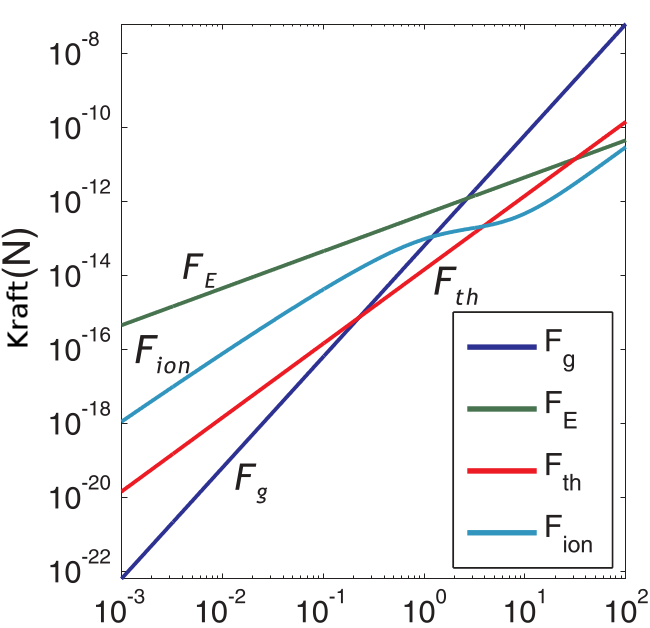
\includegraphics[width=\textwidth,height=\textwidth]{figs/allforcesequlibriummelzerlinks.png}
						\caption{}
						\label{img:linkseq}
					\end{subfigure}
					\begin{subfigure}[t]{0.49\textwidth}
						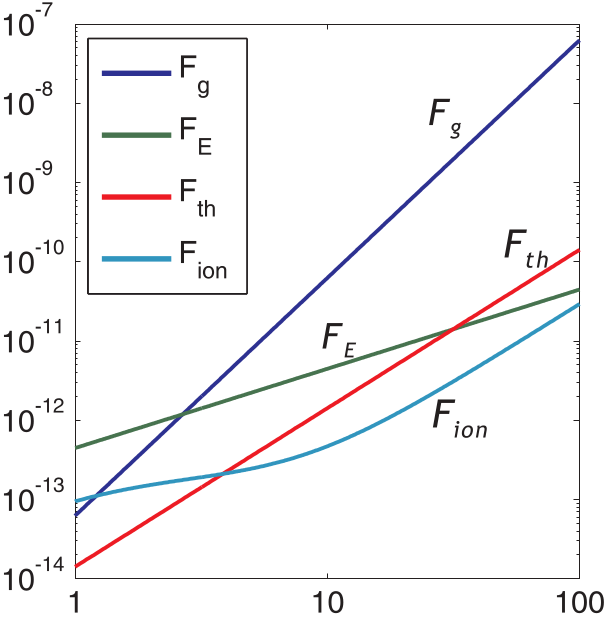
\includegraphics[width=\textwidth,height=\textwidth]{figs/allforcesequlibriummelzerrechts.png}
						\caption{}
						\label{img:rechtseq}
					\end{subfigure}
					\caption{Kräfte als Funktion des Teilchenradius in einem Argon-Plasma (Parameter: $\kappa\ix{N}=\unit[0,016]{\frac{kg m}{s^3}}$;  \mbox{$\rho\ix{S}=\unit[1,5\cdot\tenpo{3}]{\frac{kg}{m^3}}$}; $T\ix{e}=\unit[2]{eV}$; $\Phi\ix{fl}=\unit[-4]{V}$; $E=\unit[1000]{\frac{V}{m}}$; $n\ix{I}=\unit[\tenpo{15}]{m^{-3}}$; $u\ix{I}=v\ix{th,I}=v\ix{th,N}=\unit[400]{\frac{m}{s}}$, nach \cite{Melzer12}) }
					\label{img:kräfte}
				\end{figure}

			In \ref{img:kräfte} sind einige der bisher beschriebenen Kräfte für typische Parameter berechnet und mit einer doppelt-logarithmischen Skala dargestellt worden.\\
			Für Teilchen mit einem Radius im Bereich von einigen $\unit{\upmu m}$ sind die Kräfte des äußeren elektrischen Feldes $F\ix{E}$ und der Gravitation $F\ix{G}$ dominant. Daher müssen, für einen praktikablen Einfang, diese beiden Kräfte im Gleichgewicht sein, d.h. sich stationär aufheben. Dies ist gerade in der nahen Randschicht der (getriebenen) Elektrode der Fall, da dort $F\ix{E}$ stark genug ist. Weil $\grad{E}/E\ll1$ ist, trifft das nur in einem kleinen Bereich zu. Für die Neutralgasreibung $F\ix{N}$ gilt, dass diese bei großen thermischen Geschwindigkeiten des Staubes nahezu konstant wird, jedoch für "`kalten"' Staub mit zunehmendem Drift $v\ix{S}$ an Einfluss gewinnt. Die Ionenreibung $F\ix{ion}$ ist unter diesen Umständen vergleichsweise klein.\\
			In \ref{img:kräfterichtungen} sind schematisch die Kräfte aus \ref{img:kräfte} mit ihren Orientierungen dargestellt worden. Abbildungsteil \fett{(a)} zeigt dabei den Einfang von $\unit{\upmu m}$-großen Teilchen in der kleinen, lokalisierten Randschicht, wie es im diesem Experiment der Fall ist. Diese ordnen sich dabei in ausgedehnten Schichten mit hexagonaler Struktur (\tilt{fcc} bzw. \tilt{bcc} für ausgedehnte 3D-Cluster) an. Die Kräfte der Thermophorese und des "`Ionenwindes"' ($F\ix{ion}$) zeigen dabei aus dem Plasma heraus in Richtung der Kammer bzw. der Elektroden. Die Ionen sind dabei bestrebt, aufgrund der ambipolaren Diffusion in der Randschicht auf die Kammerwand, den Ladungsunterschied (etwa innerhalb einer \tilt{Debye}-Länge) zwischen dem Plasma und dem Gehäuse auszugleichen. Das liegt u.a. an den unterschiedlichen Beweglichkeiten der Ladungsträger und deren Strömung auf die Kammer (siehe Abschn. \ref{sub:rand}). Weiterhin gilt ähnliches für die thermophoretische Kraft: das aufgeheizte Plasma erzeugt einen Impulsübertrag in Richtung der kühleren Kammer, woraus eine Kraft vom Plasma weg folgt. Der Staub wird somit in einem Teil der Entladung eingefangen, in dem diese Kräfte eine untergeordnete Rolle spielen. Die relevante elektrische Feldkraft ist besonders in der Nähe der Elektroden groß und kann damit dort Gravitationskraft bzw. $F\ix{th}$ und $F\ix{ion}$ kompensieren. Sie zeigt zudem in Richtung des Plasmas, da dieses in der Randschicht nicht mehr als neutral betrachtet werden kann.

%			Für $a\gg\unit[1]{\upmu m}$ wird $F\ix{E}$ weniger relevant und es übt die Thermophorese eine immer größere Kraft auf den Staub aus. Genauer: $F\ix{th}$ ist in Experimenten, wie  sogar schon für $\grad{T}\approx \unit[2]{\frac{K}{m}}$ eine wichtige, nicht vernachlässigbare Größe.
%			Sind die Staubpartikel klein, d.h. haben einen Radius $a\approx\unit[\tenpo{-9}]{m}$, so wird die Gravitationskraft mit ihrem Einfluss $\propto a^3$ sehr klein und spielt damit kaum noch eine Rolle. Damit muss die Kraft des elektrischen Feldes mit der Ionenreibung bzw. der Thermophorese balanciert werden.

				\begin{figure}
					\centering
					\begin{subfigure}[b]{0.45\textwidth}
						\hspace{0.3cm}
						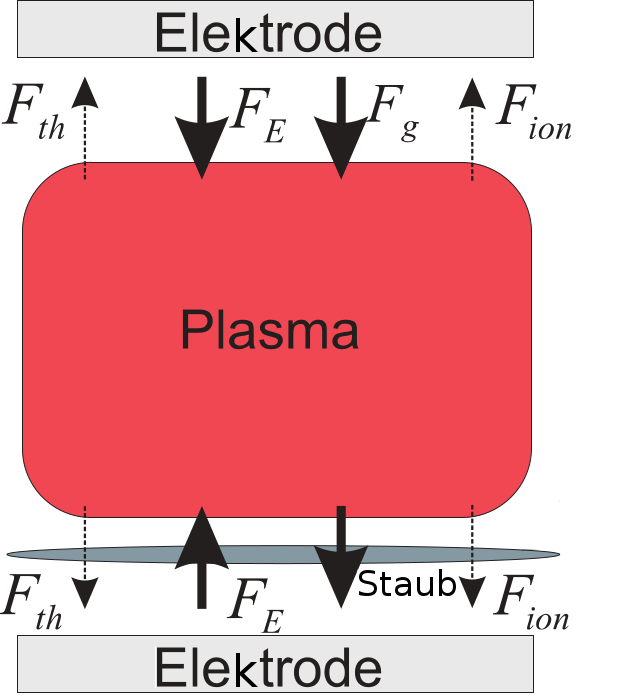
\includegraphics[width=\textwidth,height=\textwidth]{figs/directionsofforcesandtrappingmelzerlinks.png}
						\caption{}
						\label{img:linksdirection}
					\end{subfigure}
					\begin{subfigure}[b]{0.45\textwidth}
						\hspace{-0.2cm}
						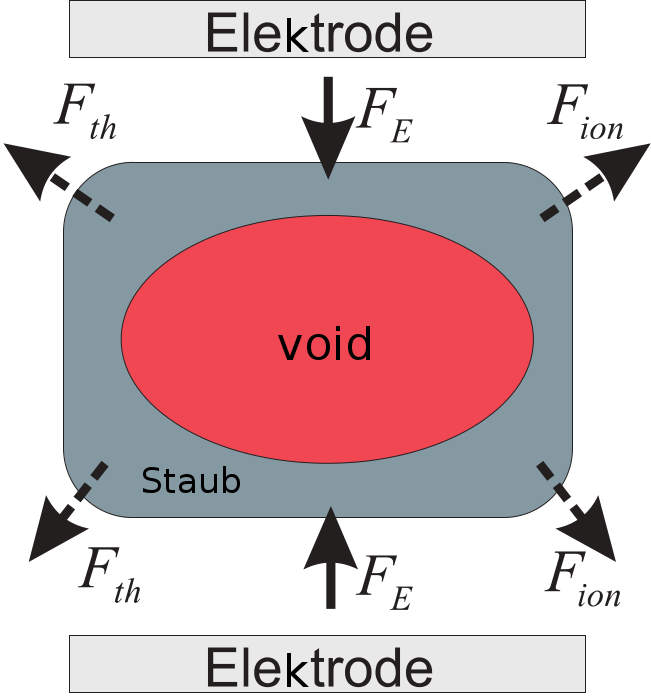
\includegraphics[width=\textwidth,height=\textwidth]{figs/directionsofforcesandtrappingmelzerrechts.png}
						\caption{}
						\label{img:rechtsdirection}
					\end{subfigure}
					\caption{Schemata für dein Einfang von Staub mit \fett{(a)}: $a\approx\unit[\tenpo{-}]{m}$ (\fett{b)}: $a\approx\unit[\tenpo{-7}]{m}$ bzw. unter Mikrogravitation. Es wurden die wichtigsten Kräfte und deren Richtungen eingezeichnet (nach \cite{Melzer12}).}
					\label{img:kräfterichtungen}
				\end{figure}

			Im zweiten Teil (b) von \ref{img:kräfterichtungen} ist ein Plasma mit Staubteilchen im $\unit{nm}$-Bereich unter Schwerelosigkeit gezeigt. Dabei entsteht der sog. \tilt{void}, welcher ein Fremdteilchen-freier Bereich in Mitten der Entladung ist und aufgrund der relativen Orientierungen der Kräfte zustande kommt. Für detailliertere Ausführungen siehe \cite{Dorier95}, \cite{Morfill99} und \cite{Goree99a}.

%            Thermophorese und Ionenwind-Kraft zeigen (selbe Argumentation wie zu Teil \fett{(a)}) aus der 'Mitte' des Plasma in Richtung der Kammer und der Elektroden, wobei von diesen aus die elektrische Feldkraft zum \tilt{void} zeigt. Da in diesem Fall $F\ix{G}$ sehr klein ist (wegen $\propto a^3$), muss für den Einfang des Staubes das starke $F\ix{E}$, welches zwischen Kammer und Plasma entsteht, mit $F\ix{th}$ und $F\ix{ion}$ im Gleichgewicht sein. Somit ist es m\"oglich, Staub in dreidimensional ausgedehnten Bereichen in der gesamten Entladung einzufangen.\\ Es stellen sich sogar Dichte- bzw. Volumen- und Massegradienten aufgrund der empfindlichen Abhängigkeit von Gravitation und elektrischer Feldkraft ein. Das bedeutet, dass sich schwerere, größere Teilchen bzw. "`verschmolzene"' Partikelcluster am Rande des Einfangs wiederfinden, wohingegen kleinerer Staub sich dicht gepackt um den \tilt{void} herum befindet.

		\subsection{Finite Yukawa-Cluster}\label{sub:yukawaclust}

				\begin{figure}
					\centering
					\begin{subfigure}[b]{0.3\textwidth}
						\centering
						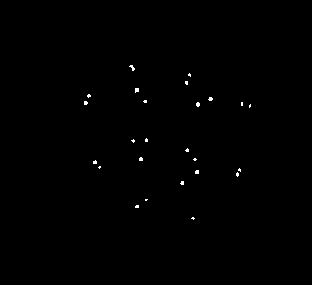
\includegraphics[width=\textwidth,height=\textwidth]{figs/rot00013ungestrt.png}
						\caption{}
						\label{img:rechts}
					\end{subfigure}
					\begin{subfigure}[b]{0.3\textwidth}
						\centering
						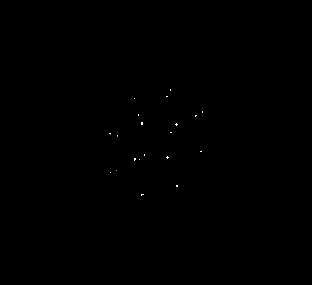
\includegraphics[width=\textwidth,height=\textwidth]{figs/gruen05006ungestrt.png}
						\caption{}
						\label{img:links}
					\end{subfigure}
					\begin{subfigure}[b]{0.3\textwidth}
						\centering
						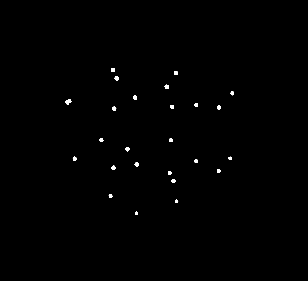
\includegraphics[width=\textwidth,height=\textwidth]{figs/gelb00011ungestrt.png}
						\caption{}
						\label{img:oben}
					\end{subfigure}
					\caption{Aufnahmen aus 3 verschiedenen, orthogonalen Raumrichtungen eines \tilt{Yukawa-Balls} mit $N=26$ Teilchen. Das System befindet sich bei niedrigen Gasdrücken ($\approx\unit[6-10]{Pa}$) in einer Argon-Entladung unter einem Kupferring, welcher sich im Plasma auf $\Phi\ix{fl}$ aufgeladen hat. \fett{(a)}: Ansicht aus der Ebene des Clusters \fett{(b)}: von oben \fett{(c)}: andere Richtung in der Ebene}
				\end{figure}

			Bisher wurden in den Abschnitten \ref{sub:kaprfplasm} und \ref{sub:rand} allgemein gültige Charakteristika des für diesen Aufbau verwendeten Plasmas besprochen. Außerdem sind in \ref{sub:ströme} und \ref{sub:dynamik} die für komplexe bzw. staubige Plasmen spezifischen Kenngrößen und Prozesse, wie beispielsweise Aufladung und Einfang, beschrieben worden. Damit kennen wir die Dynamik eines einzelnen Staubteilchen in einem Plasma und unter welchen Bedingungen ein Einfang gegeben ist, jedoch wissen wir nichts über das kollektive Verhalten der bereits besprochenen \tilt{Yukawa-Cluster}. Wann und wo sind diese - falls ein solcher Zustand existiert - stabil? Wie ist ihr Verhalten bei Störungen des externen Potentials? Dieser Abschnitt soll sich mit diesen Fragen, in Bezug auf einen Versuch unter den Bedingugen aus \ref{img:linksdirection}, auseinander setzen.

				 \subsubsection{Struktur}

						 \begin{figure}
						 	\centering
						 	\begin{subfigure}[t]{0.48\textwidth}
						 		\centering
						 		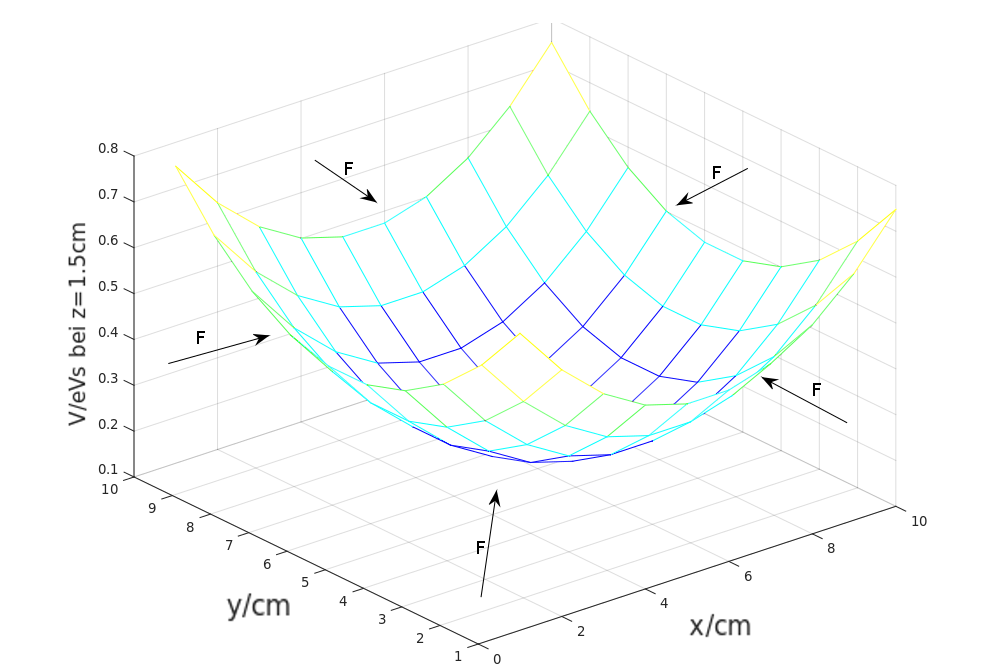
\includegraphics[width=1.1\textwidth,height=0.3\textheight]{figs/einfangpotnu.png}
						 		\caption{}
						 		\label{img:potential}
						 	\end{subfigure}
						 	\begin{subfigure}[t]{0.48\textwidth}
						 		\centering
						 		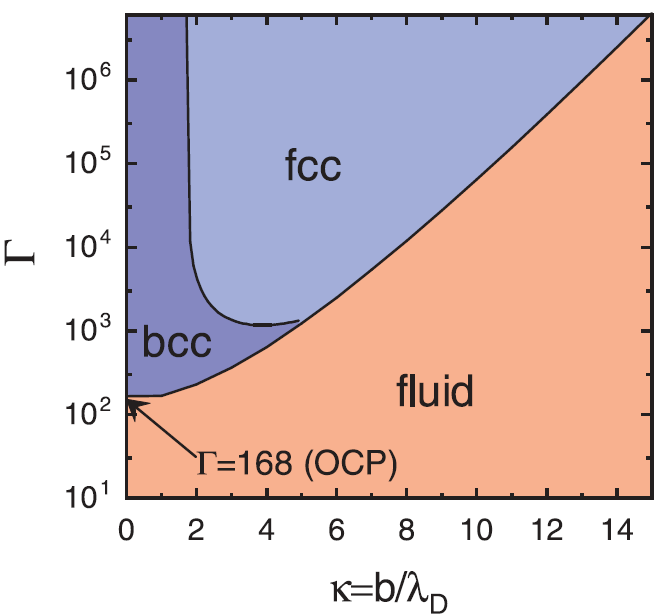
\includegraphics[width=0.9\textwidth,height=0.3\textheight]{figs/gammaphasetransmelzer.png}
						 		\caption{}
						 		\label{img:gamma}
						 	\end{subfigure}
						 	\caption{\fett{(a)}: Harmonischer Einfang des Potentials $V$ in $\unit{eVs}$ mit globalem Minimum (dunkel). Darstellung für eine Elektrodenhöhe (siehe später Abschnitt \ref{sub:einfang}) von $\unit[1,5]{cm}$. \fett{(b)}: Phasendiagramm nach \cite{Melzer12} für eine effektive Coulomb-Kopplung nach Gl. (\ref{eq:kopplung}).}
						 \end{figure}

%							\begin{wrapfigure}{r}{0.5\textwidth}
%								\begin{minipage}{0.2\textwidth}
%									\caption{\underline{\fett{oben}:} $N=190$-Cluster; Teilchen-Verteilung. \underline{\fett{unten}:} Vierte Schale mit penta- und hexagonalen Zellen, sowie Defekten (weiß).}\label{img:strukturN190}
%								\end{minipage}
%								\begin{minipage}{0.23\textwidth}
%									\centering
%									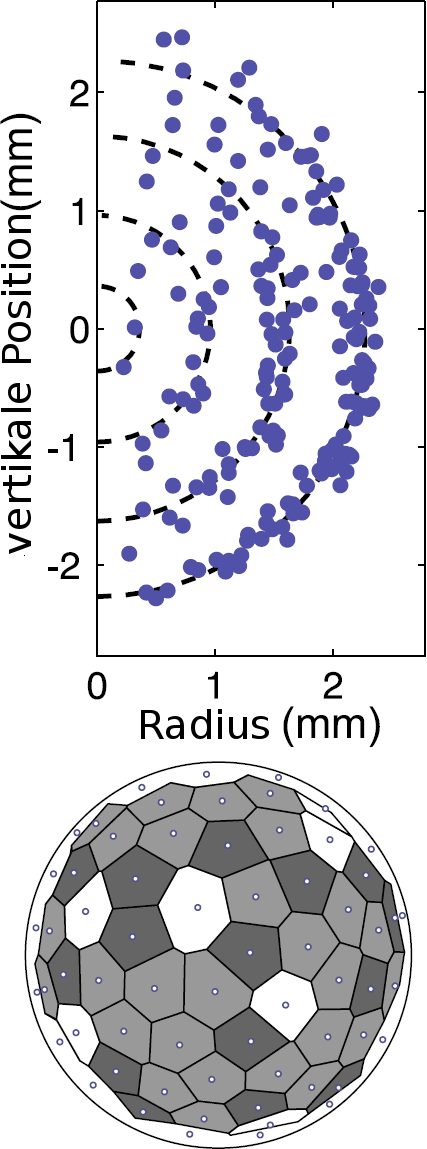
\includegraphics[width=\textwidth,height=2.6\textwidth]{figs/yukawaballN190.png}
%								\end{minipage}
%							\end{wrapfigure}

					 Ein \tilt{Yukawa-Ball} kann durch das Erzeugen eines externen Potentials eingefangen werden: beispielsweise durch räumliche Begrenzung mit einer Küvette oder einem Ring, welche sich im Plasma aufladen und damit eine nach innen gerichtete, elektrische Kraft auf den ebenfalls negativ geladenen Cluster ausüben. Das aus den Kräften auf die Staubpartikel resultierende Potential kann als harmonisch angenommen werden, e.g.:

						 \begin{align}
						 	V\left(\vec{r}\ix{j}\right)=\frac{m\ix{S}\omega\ix{0}^2}{2}\begin{pmatrix} 1 \\ \alpha\ix{y}  \\ \alpha\ix{z} \end{pmatrix} \vec{r}\ix{j}^2 \,\, ,
						 \end{align}

					wobei $\alpha\ix{k}=\omega\ix{k}^2/\omega\ix{x}^2$ die relative der Richtung $k\in\left\lbrace x,y,z\right\rbrace$ und $\omega\ix{0}=\omega\ix{x}$ die absolute Einfangstärke ist. In \ref{img:potential} ist das Potential, in dessen globalen Minimums sich der Cluster in diesem Experiment bildet, für eine feste Höhe über der getriebenen Elektrode dargestellt. Für eine geeignete Anordnung strebt man einen isotropen Einfang mit $\omega\ix{x}=\omega\ix{y}=\omega\ix{z}$ an. Ein finiter Yukawa-Cluster hat die Struktur konzentrischer Kugelschalen, welche mit steigendem Radius auch mit immer mehr Teilchen besetzt sind. Ein Visualisierung ist für $N=190$ in \ref{img:strukturN190} gezeigt.

						\begin{align}
							\Gamma=\frac{Z\ix{S}e^2}{4\pi\varepsilon\ix{0}b\ix{WS}k\ix{B}T\ix{S}}  \,\,; \quad \Gamma\ix{C,eff}=\Gamma\exp\left(-\frac{b\ix{WS}}{\lambda\ix{D}}\right) \label{eq:kopplung}
						\end{align}

						\begin{wrapfigure}{r}{0.25\textwidth}
							\centering
							\vspace{-0.5cm}
							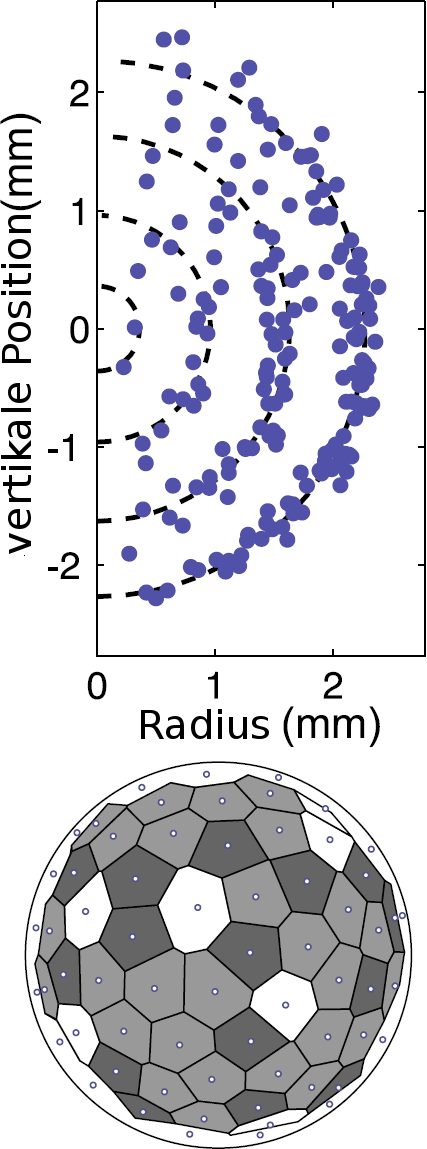
\includegraphics[width=0.22\textwidth,height=0.55\textwidth]{figs/yukawaballN190.png}
							\caption{\underline{\fett{oben}:} $N=190$-Cluster; Teilchen-Verteilung. \underline{\fett{unten}:} Vierte Schale mit penta- und hexagonalen Zellen, sowie Defekten (weiß) (nach \cite{Arp04}).}\label{img:strukturN190}
						\end{wrapfigure}

                    Um ein Maß für die Stabilität eines staubigen Plasmas zu erhalten, geht man, wie bei Festkörpern und deren Elektronengasen, von einer Punktladung $Q$ vor dem Hintergrund der Ionen und Elektronen aus (\tilt{one component plasma} - OCP). Der Kopplungsparameter $\Gamma$ in Gl. (\ref{eq:kopplung}) beschreibt somit die elektrostatische Wechselwirkung eines Teilchens mit seinen Nachbarn in Einheiten der thermischen Energie.\\
					Für ein $\Gamma>1$ spricht man von einer starken Kopplung innerhalb des Clusters bzw. des Plasmas. Mit $\Gamma\geq\Gamma\ix{k}$ liegen kristalline Systeme vor. Bei einem kleineren Wert gehen die Cluster in einen flüssigen bzw. gasförmigen Zustand über (\ref{img:gamma}). Das heißt, dass ein System aus Staubpartikeln "`schmelzen"' kann, bringt man durch Lasereinstrahlung o.ä. gezielt Energie in den Cluster ein und verringert damit die Ordnung bzw. erhöht die thermische Bewegung. Dabei verschwindet zuerst die Winkelabhängigkeit, was das Auflösen der kristallartigen Strukturen innerhalb des Clusters zur Folge hat (zum Beispiel \cite{Thomas96}).\\
					Die größe $b\ix{WS}=\left(3/4\pi n\ix{S}\right)^{-1/3}$ ist der \tilt{Wigner-Seitz}-Radius: er ist analog zu $\overline{b}$ aus Tab. \ref{tab:kenngroessen} eine Skala für Teilchenabstände. Insbesondere ist $b\ix{WS}$ eine korrektere Größe, da sich der Staub in hexagonalen bzw. pentagonalen Zellen auf den konzentrischen Sphären des Clusters anordnet. Die Zusammensetzung eines solchen \tilt{finiten Yukawa-Systems} ist in \ref{img:strukturN190} dargestellt. Außerdem: sowohl aufgrund der bisher besprochenen Kräfte und der Coulomb-Wechselwirkung des Staubes, als auch wegen des nicht-reziproken \tilt{Ionenfokus} (siehe \cite{Melzer95c}) streben die Systeme bei entsprechenden Umgebungsparametern eine energetisch günstige, kristallartige Struktur an. \\
					Der effektive Parameter für Coulomb-Wechselwirkungen $\Gamma\ix{C,eff}$ entspricht einer modifizierten Kopplung mit Rücksicht auf die Abschirmung durch die Ionenwolke (\cite{Lampe00}, \cite{Schweigert00d}) um ein Partikel bzw. den Cluster. Aus diesem Grund führt man die Abschirmstärke $\kappa=b\ix{WS}/\lambda\ix{D}$ ein, welche angibt, um wie viel die elektrostatische Wechselwirkung mit einem Teilchen der Ladung $Q$ innerhalb einer Elementarzelle der Staubpartikel abgeschwächt ist. Außerdem folgt daraus der Zusammenhang für die Phasengrenze in \ref{img:gamma} $\Gamma\left(\kappa\right)$: für große \tilt{Wigner-Seitz}-Radien bzw. sehr kleine Debye-Längen verschwindet die Wechselwirkung zwischen den Staubteilchen nahezu vollständig. Das Potential geht für diesen Fall in das aus dem Modell harter Kugeln über (bspw. van-der-Waals-Gastheorie etc.).\\
					Abschließend sei erwähnt, das die bisher genannten Eigenschaften u.U. stark von der Art der Wechselwirkung bzw. der Teilchenzahl abhängen: die Betrachtungen gehen von reiner Coulomb- oder Yukawa-Wechselwirkung aus. Die Besetzungszahlen der Sphären des Clusters können jedoch für die verschiedenen Potentiale stark variieren, was u.a. eine Folge unterschiedlicher Abschirmungen ist.

				\subsubsection{Dynamik- und Modenanalyse} \label{subsub:moden}

					Auf Grundlage der Überlegungen zur Wechselwirkung und des Einfangs eines finiten Yukawa-Systems, kann nun eine Analyse der dynamischen Eigenschaften dessen erfolgen. Diese beruht auf der Entwicklung eines \tilt{Modenspektrums} dieses Clusters, wobei im Gegensatz zu ausgedehnten System darin nur eine endliche Zahl von Moden vorhanden sind. Statt einer Dispersionsrelation für Wellen bestimmt man demnach Schwingungsmoden, welche den Grenzen und Randbedingungen des Clusters bzw. des Einfangs genügen.\\
					Mit der Normierung auf Abstandseinheiten $r\ix{0}$ und Energieeinheiten $E\ix{0}$ folgt Gl. (\ref{eq:energie}). Die erste Summe stellt den kinetischen Anteil der Energie des $i$-ten Teilchens im Rahmen eines harmonischen Oszillators dar. Die Yukawa-Abstoßung im zweiten Teil kommt aus der elektrostatischen Wechselwirkung innerhalb des Staubkristalls, weswegen $\kappa=r\ix{0}/\lambda\ix{D}$ und $r\ix{ij}=|\vec{r}\ix{i}-\vec{r}\ix{j}|$ gilt.

						\begin{align}
							E=\sum_{i=1}^{N}\vec{r}\ix{i}\,^2+&\sum_{i<j}^{N}\frac{\exp\left(-\kappa r\ix{ij}\right)}{r\ix{ij}} \label{eq:energie} \\
							r\ix{0}=\left(\frac{2Z\ix{S}^2e^2}{4\pi\varepsilon\ix{0}m\ix{S}\omega\ix{0}^2}\right)^{1/3} \quad &\quad E\ix{0}=\left(\frac{Z\ix{S}^2e^4m\ix{S}\omega\ix{0}^2}{8\pi\varepsilon\ix{0}}\right)^{1/3} \nonumber
						\end{align}

					Ausgehend von der normierten Gesamtenergie $E$ eines N-Teilchen-Clusters lässt sich, als Analogon zur Taylor-Entwicklung, durch Approximation um ein Equilibrium die sog. \tilt{Hesse-Matrix} in Gl. (\ref{eq:matrix}) als dynamische Matrix $A\in\text{Mat}\left(3N\times3N\right)$ aufstellen. Hinter dieser Formulierung steht die Idee, dass jede Bewegung als anteilige Überlagerung der Schwingungsmoden verstanden werden kann. Somit steht in $A$ für alle Teilchenkoordinaten $i,j$ die 2. Ordnung der Entwicklung um das Gleichgewicht. Löst man für diese das Eigenwertproblem (\cite{Schweigert95c}), so erhält man mit $\vec{\nu}\ix{p}$ und $\omega\ix{p}$ den Modenvektor und -frequenz der Mode $p$.

						\begin{align}
							A=
							\begin{pmatrix}
							\frac{\partial^2 E}{\partial x\ix{i} \partial x\ix{j}} & \cdots & \frac{\partial^2 E}{\partial x\ix{i} \partial z\ix{j}} \\ 
							\vdots & \ddots & \vdots \\ 
							\frac{\partial^2 E}{\partial z\ix{i} \partial x\ix{j}} & \cdots & \frac{\partial^2 E}{\partial z\ix{i} \partial z\ix{j}}
							\end{pmatrix} 
							\quad \text{mit} \quad \frac{\partial^2 E}{\partial x\ix{i}\partial y\ix{j}}&=
							\begin{pmatrix}
							\frac{\partial^2 E}{\partial x\ix{1} \partial x\ix{1}} & \cdots & \frac{\partial^2 E}{\partial x\ix{1} \partial y\ix{N}} \\ 
							\vdots & \ddots & \vdots \\ 
							\frac{\partial^2 E}{\partial x\ix{N} \partial y\ix{1}} & \cdots & \frac{\partial^2 E}{\partial x\ix{N} \partial y\ix{N}}
							\end{pmatrix}
							\label{eq:matrix} \\
							\left(A-\omega\ix{p}^2I_{(3N)}\right)\vec{\nu}\ix{p}&=0 \label{eq:ewp} \\ 
							\text{wobei} \quad \vec{\nu}\ix{p}^\top=\left(x\ix{1,p},\dots,x\ix{N,p},y\ix{1,p},\dots\right) \quad &\text{bzw.} \quad \vec{\nu}\ix{i,p}^\top=\left(x\ix{i,p},y\ix{i,p},z\ix{i,p}\right) \nonumber
						\end{align}

					Aus der Lösung von Gl. (\ref{eq:ewp}) um $A$ erhält man folglich $3N$ Modenfrequenzen und -vektoren. Den Anteil, den eine jede Mode $p$ an der Bewegung eines Teilchens $i$ hat, erhält man durch die Projektion des Vektors der Geschwindigkeit $\vec{v}\ix{i}\left(t\right)$ auf die Modenvektoren $\vec{\nu}\ix{i,p}$. Anders herum: den Anteil der Mode an der Clusterbewegung, ob thermisch oder extern angeregt, erhält man aus der Summe aller Anteile an den Teilchenbewegungen (siehe Gl. (\ref{eq:summe}), \cite{Melzer03}). Die Energie, welche in der Mode $p$ bei der Frequenz $\omega$ gespeichert ist, ergibt sich über die Fouriertransformation dieses Bewegungsanteils zu $S\ix{p}\left(\omega\right)$.

						\begin{align}
							f\ix{p}&\left(t\right)=\sum_{i=1}^{N}\vec{v}\ix{i}\left(t\right)\vec{\nu}\ix{i,p} \label{eq:summe} \\
							S\ix{p}\left(\omega\right)&=\left.\left.\frac{2}{T}\right|\int_{0}^{T}f\ix{p}\left(t\right)\exp\left(-\imag\omega t\right)\diff t\right|^2 \label{eq:energiedicht}
						\end{align}

						\begin{figure}
							\centering
							\begin{subfigure}[b]{0.48\textwidth}
								\centering
								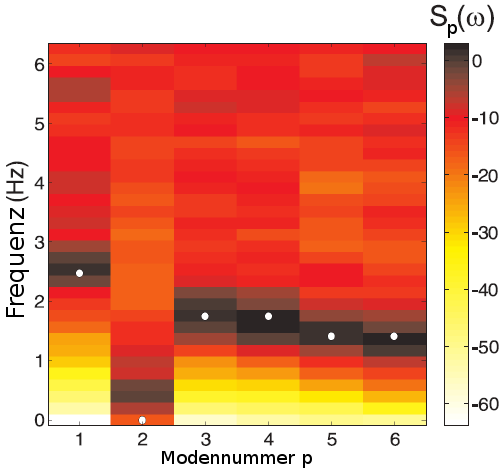
\includegraphics[width=\textwidth,height=0.3\textheight]{figs/modenvenergie3teilchenmelzer.png}
								\caption{}
								\label{img:spektrum}
							\end{subfigure}
							\begin{subfigure}[b]{0.48\textwidth}
								\centering
								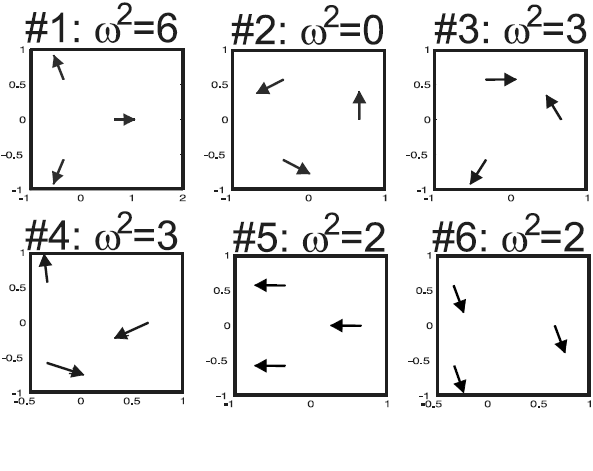
\includegraphics[width=\textwidth,height=0.3\textheight]{figs/modenvektoren3teilchenmelzer.png}
								\caption{}
								\label{img:moden}
							\end{subfigure}
							\caption{\fett{(a)}: Modenspektrum für einen 3-Teilchen-Cluster. Die weißen Punkte entsprechen theoretisch errechneten Werten der Modenfrequenzen. Die Bereiche von $S\ix{p}\left(\omega\right)\rightarrow0$ treten bei der Eigenfrequenz auf. \fett{(b)}: Eigenvektoren ($\vec{\nu}\ix{i,p}$) für $N=3$. Die Modenfrequenz ist auf die Einfangstärke $\omega\ix{0}$ normiert (nach \cite{Melzer12}).}
						\end{figure}

					Die spektrale Energiedichte aus Gl. (\ref{eq:energiedicht}) wird in \ref{img:spektrum} für einen sehr simplen Cluster aus $N=3$ Teilchen dargestellt. Passend dazu sind in \ref{img:moden} die Modenvektoren der drei Staubpartikel eingezeichnet. Insbesondere sind dort Moden gezeigt, welche allgemein für alle Cluster auftreten: \tilt{breathing}, \tilt{slosh} und Rotation. $p=1$ zeigt die \tilt{breathing}-Mode: alle Teilchen entfernen sich vom Clusterschwerpunkt, wobei dieser jedoch fest bleibt. Die Frequenz $\omega\ix{breath}$ hängt schwach von $N$ ab und steigt mit der Abschirmung $\kappa$. Mode $p=2$ ist die Rotationsmode. Ihre Eigenfrequenz ist $0$, da es für diese keine rückstellenden Kräfte gibt. In $p=3$ und $p=4$ sind \tilt{kink}-Moden gezeigt. Nummer 5 und 6 stellen \tilt{slosh}-Moden dar: das System führt eine Schwerpunktstranslation aus, wobei alle Partikel sich in die selbe Richtung bewegen.\\
					Diese \tilt{Normalmodenanalyse} ist ein geeignetes Mitte zur Analyse der Dynamik eines finiten Systems (siehe \cite{Melzer01},\cite{Melzer03}), vorausgesetzt es genügt den gemachten Voraussetzungen: Yukawa-Wechselwirkung, starke Kopplung, homogene Partikel \dots

				\subsubsection*{Fluidmoden}

					Genau wie in der, diesem Teilgebiet übergeordneten Plasmaphysik, lässt sich ein finiter Cluster als hydrodynamische Gesamtheit auffassen. Ähnlich wie beim \tilt{Fluidmodell} und der Betrachtung durch die \tilt{magnetohydrodynamischen Gleichugen} (MHD), nimmt man hierbei das System als kontinuierliche Masse mit entsprechender Ladungsverteilung an. Daraus ergeben sich neue Möglichkeiten die Dynamik des Cluster zu beschreiben und nachzuvollziehen.\\
					Eingangs muss das neue Potential $\Phi\left(\vec{r},t\right)$ des fluiden "`Tropfens"' beschrieben werden. Da der Cluster von Ladungsträgern abgeschirmt wird, welche sich um diesen auf Grund seiner elektrostatischen Wechselwirkung ansammeln - analog zu den vorherigen Abschnitten -, kann man die modifizierte Poissongleichung (Gl. (\ref{eq:poisson})) für die Ladungsdichte $\rho\left(\vec{r},t\right)$ des Systems benutzen. Deren Lösung erhält man mit der \tilt{Green-Funktion} $G\left(\vec{r}\right)$ aus Gl. (\ref{eq:green}) in (\ref{eq:fluid}). 

						\begin{align}
							&\left(\Delta-\kappa^2\right)\Phi\left(\vec{r},t\right)=\frac{1}{\varepsilon\ix{0}}\rho\left(\vec{r},t\right) \label{eq:poisson} \\
							\Phi\left(\vec{r}\right)&=\int_{\mathbb{R}^3}\frac{\rho\left(\vec{r}\,^\prime,t\right)}{4\pi\varepsilon\ix{0}|\vec{r}-\vec{r}\,^\prime|}\diff^{3}r^\prime \\
							&\,\,\,\,\vdots\quad G\left(\vec{r}\right)=\frac{\exp\left(-\kappa|\vec{r}|\right)}{4\pi|\vec{r}|} \label{eq:green}\\
							\Phi\left(\vec{r}\right)&=\int_{\mathbb{R}^3}\frac{\exp\left(-\kappa|\vec{r}-\vec{r}\,^\prime|\right)}{4\pi\varepsilon\ix{0}|\vec{r}-\vec{r}\,^\prime|}\rho\left(\vec{r}\,^\prime,t\right)\diff^{3}r^\prime \label{eq:fluid}
						\end{align}

					Die Green-Funktion entspricht einem einheitenlosen Yukawa-Potential, welches man nach \cite{Arfken05},\cite{Yap10} in eine Reihe von sphärisch-harmonischen \tilt{Kugelflächenfunktionen} $Y_{lm}\left(\theta,\varphi\right)$ und \tilt{modifizierten Besselfunktionen} $i_{l}\left(x\right)$ und $k_{l}\left(x\right)$ entwickeln kann. Die Definitionen erfolgen in dreidimensionalen Kugelkoordinaten $\left(r,\theta,\varphi\right)$, wobei die minimalen bzw. maximalen Abstände $r\ix{<}=\min\left(r^\prime,r\right)$ und $r\ix{>}=\max\left(r^\prime,r\right)$ sind.

						\begin{align}
							\frac{\exp\left(-\kappa|\vec{r}-\vec{r}\,^\prime|\right)}{4\pi|\vec{r}-\vec{r}\,^\prime|}=\sum_{l=0}^{\infty}\sum_{m=-l}^{l}\frac{r\ix{<}^l}{r\ix{>}^{l+1}}i_{l}\left(\kappa r\ix{<}\right)k_{l}\left(\kappa r\ix{>}\right)\exp\left(-\kappa r\ix{>}\right)Y_{lm}^*\left(\theta^\prime,\varphi\prime\right)Y_{lm}\left(\theta,\varphi\right) \label{eq:entwick}
						\end{align}

					Nach \cite{Ivanov09} und \cite{Schella13} lassen sich aus Gl. (\ref{eq:entwick}) die Multipolmomente der Ladungsdichte des Clusters gewinnen (siehe Gl. (\ref{eq:multipol})). Die Indizes $lm$ geben die Modenzahlen an, wobei analog zu den Zust\"anden eines Wasserstoff-artigen Atoms $\Psi\left(\vec{r}\right)=L_{n}\left(r\right)Y_{lm}\left(\theta,\varphi\right)$ diese die Symmetriezahlen bzw. -richtungen der Schwingungen des "`Tropfens"' angeben (siehe \ref{img:fluidmode}).

						\begin{align}
							\rho_{lm}\left(t\right)=&\sqrt{\frac{4\pi}{2l+1}}\int_{\mathbb{R}^{3}}\rho\left(\vec{r},t\right)i_{l}\left(\kappa r\right)Y^{*}_{lm}\left(\theta,\varphi\right)\diff^{3}r \label{eq:multipol} \\
							Q_{lm}\left(\omega\right)=&\left.\left.\frac{2}{TN}\right|\int_{0}^{T}\rho_{lm}\left(t\right)\exp\left(-\imag\omega t\right)\diff t\right|^{2}
						\end{align}

					Wie in Gl. (\ref{eq:energiedicht}) wird \"uber die Fouriertransformation aus dem Zeit- in den Frequenzraum die anteilige Energie der Mode $q_{lm}$ an der Schwingungsbewegung des Tropfens bei $\omega$ in der korrespondierenden Periode  $T$ berechnet (\cite{Schella13}). Das Frequenzpektrum stellt somit die Zusammensetzung der Clusterbewegung aus den Moden $lm$ dar.\\
					Nach Gl. (\ref{eq:multipol}) k\"onnen die einzelnen Moden als Dipol, Quadrupol, \dots identifiziert werden. Ihren Symmetriezahlen $lm$ entsprechend, vollf\"uhrt der Cluster dabei die bereits bekannten Schwingungen (siehe \ref{subsub:moden}): die \tilt{breathing}- und \tilt{slosh}-Mode. Dabei ist das Tupel $\left(l=0,m=0\right)$ die Monopolschwingung: eine periodischen Kompression und Relaxation des Systems (\tilt{breathing}). Die Indizes $\left(l=0,m=1\right)$ und deren Permutation stellen eine Dipolschwingung dar. Der Ball vollf\"uhrt eine Schwerpunktstranslation (\tilt{slosh}) und leichte Deformation, senkrecht zur Schwingungsachse. Die Beschreibung einer Rotationsbewegung fehlt, da die Ladungsverteilung invariant gegen\"uber Drehungen ist. H\"ohere Symmetrien - Schwingungen auf 2 oder mehr Raumachsen - entsprechen demnach h\"oheren Werten von $\left(l,m\right)$. Die in diesem Versuch betrachteten Bewegungen sind Quadrupol- bzw. Dipolschwingungen.

						\begin{figure}[H]
                            \centering
                            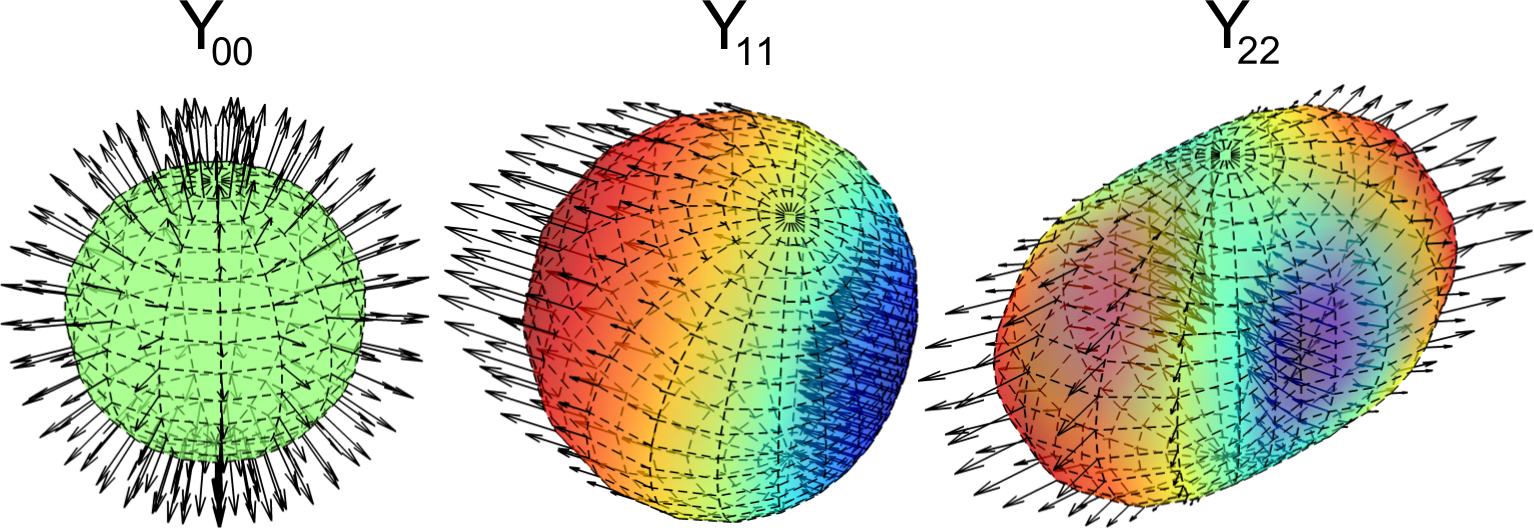
\includegraphics[width=\textwidth,height=0.375\textwidth]{figs/y001122.png}
                            \caption{Darstellung der Fluidmoden über Kugelflächenfunktionen mit Pfeilen als charakteristische Schwingungsrichtungen bzw. -achsen. Rote Bereiche sind als Regionen hoher Dichten, blaue als jene niedrigerer zu interpretieren. Von links nach rechts: Monopol (\tilt{breathing}), Dipol (\tilt{slosh}), Quadrupol (nach \cite{Mulsow13}).}
                            \label{img:fluidmode}
                        \end{figure}

	\newpage
	\begin{align*}
	\,
	\end{align*}
	\newpage

	\section{Durchführung}\label{sec:durch}

		Im anschlie{\ss}ende Abschnitt wird der Aufbau, sowie die Durchf\"uhrung und die Messmethodik des Experiments dieser Arbeit umrissen. Es folgt eine vertiefenden Beschreibung der Plasmakammer, einschlie{\ss}lich der Kameraanordnung mit Beleuchtungslasern. Eine Betrachtung des sog. \tilt{Plasma-Glow} wird ebenso Teil dieses Abschnitts sein. Zus\"atzlich soll dabei die dreidimensionale Rekonstruktion der Partikelbewegungen aus den Kamerabildern kurz beschrieben werden.

			\begin{figure}[H]
				\centering
				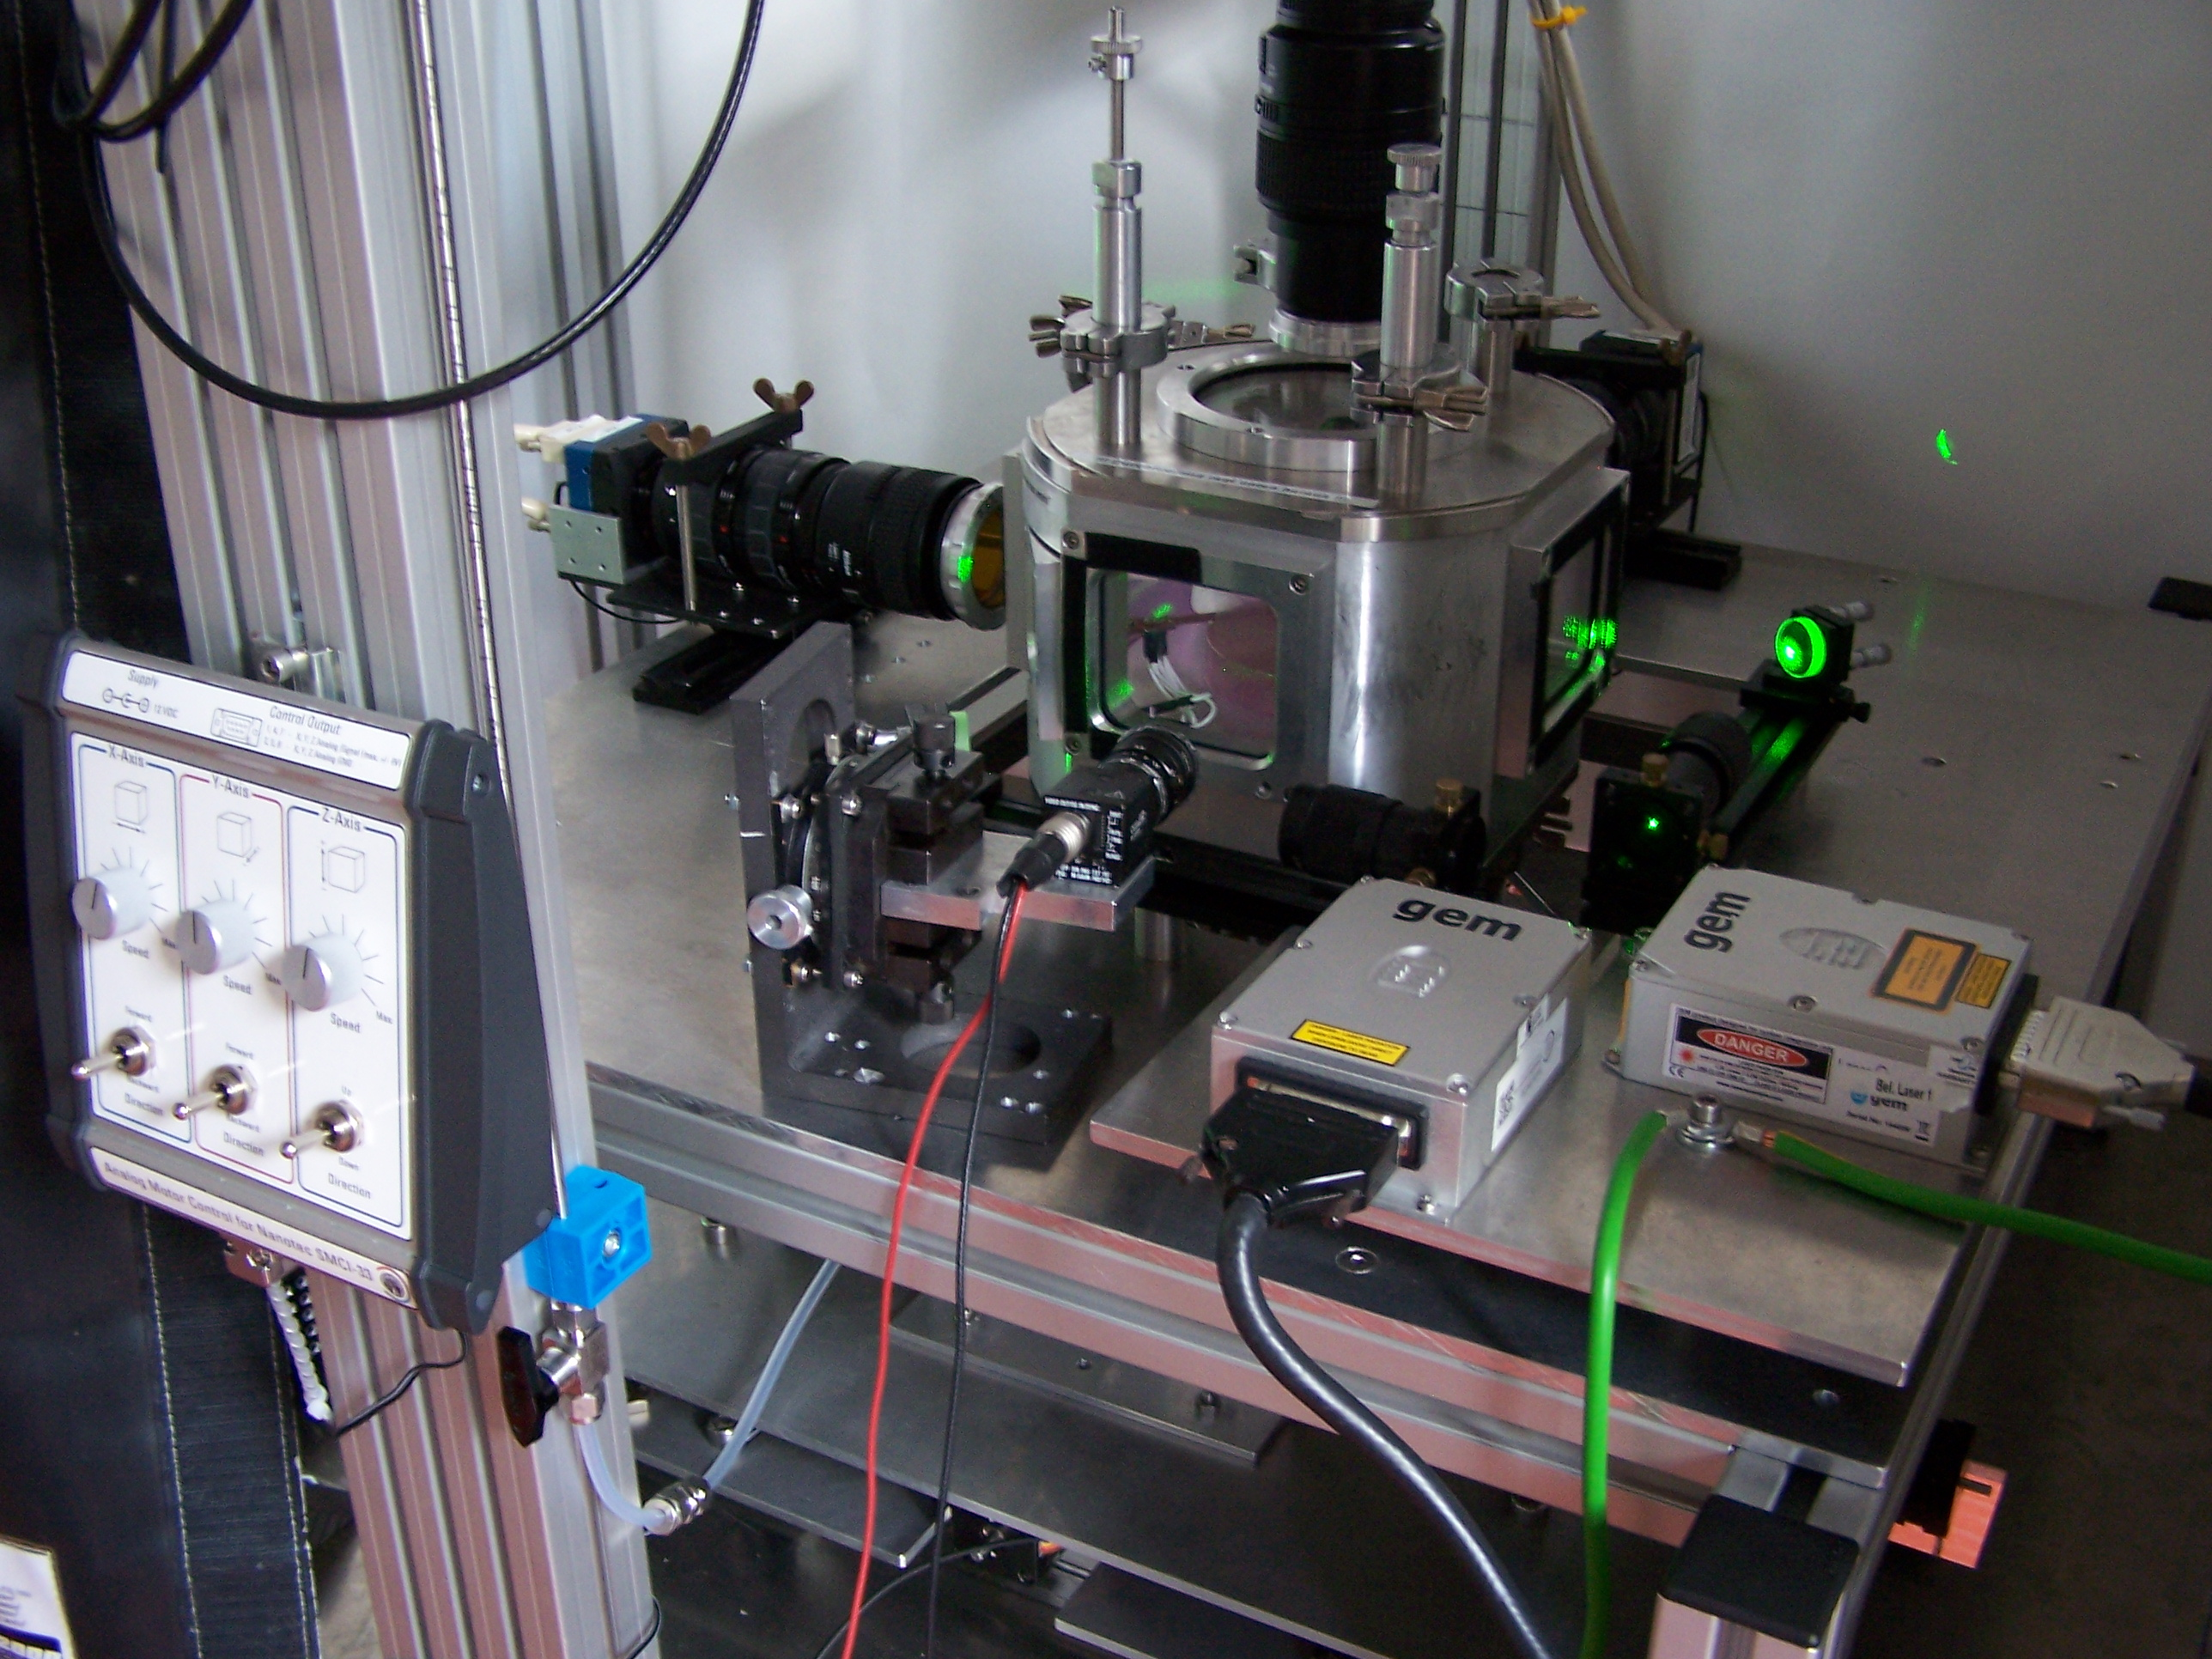
\includegraphics[width=\textwidth,height=0.7\textwidth]{figs/cam/aufbau.jpg}
				\caption{Versuchsaufbau bei eingeschaltetem Plasma mit grünen Beleuchtungslasern und verschiebbarem Tisch (siehe Steuerung links). Eine kleine Schwarz-Weiß-Übersichtskamera (Bildmitte vor der Kammer) ermöglichte auch bei laufendem Experiment die Beobachtung des Kammerinneren. Um den Versuch herum befand sich, als Sicherheitsvorkehrung, ein Laserschutzvorhang (Hintergrund).}
				\label{img:photo}
			\end{figure}

		\subsection{Aufbau}

				\begin{figure}[!t]
					\centering
					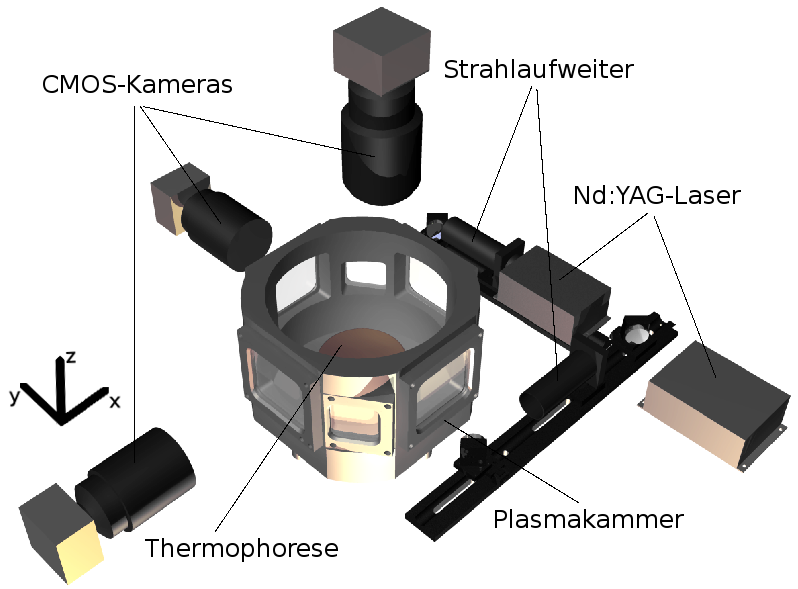
\includegraphics[width=0.75\textwidth,height=0.55\textwidth]{figs/witharrowsnunu.png}
					\caption{Schematische Ansicht des Stereoskopiesystems aus \ref{img:photo}. Das eingezeichnete Koordinatensystem (rechts unten) entspricht dem der Tischbewegung und der späteren Auswertung (nach \cite{Mulsow13}).}
					\label{img:plasmakammer}
				\end{figure}

			Die in diesem Experiment verwendete Plasmakammer ist in \ref{img:plasmakammer} gezeigt. Den fertigen Aufbau, samt Beleuchtungslaser und elektrisch verschiebbaren Versuchstisch zeigt das Photo in \ref{img:photo}. Die Kammer hat einen Innendurchmesser von $\unit[25]{cm}$, wobei deren Deckel und Boden aus Edelstahl und die Wände aus Aluminium bestehen. Vier gro{\ss}e und 2 kleine, seitlich angebrachte, antireflexbeschichtete Fenster erm\"oglichen,  aus der Ebene den Blick auf den Yukawa-Ball. Im Deckel der Kammer befindet sich ein weiteres, kreisrundes Fenster mit einem Durchmesser von etwa $\unit[9]{cm}$. Die Beobachtung der Cluster wird durch drei zueinander orthogonale Kameras realisiert, wobei diese durch die genannten Glas-Einsätze in der Kammer schauen. Das daraus entstehende stereoskopische System nutzt man letztendlich zur Rekonstruktion der Teilchentrajektorien in 3D.\\
			Wie im Abschnitt \ref{sub:kaprfplasm} beschrieben, wird in diesem Versuch ein kapazitiv gekoppeltes Niederdruck-Radiofrequenz-Plasma in einer asymmetrischen Entladungskammer erzeugt. Eine abgeschirmte Messingelektrode befindet sich im unteren Teil des Aufbaus und wird, \"uber die kapazitive Kopplung zur Anpassung von Gleistromanteilen, von einem Generator mit einer Leistung zwischen $\unit[1-3]{W}$ bei einer Frequenz von $\unit[13,56]{MHz}$ betrieben. Der \"ubrige Teil der Kammer liegt auf Massepotential und dient damit als, fl\"achenm\"a{\ss}ig um ein vielfaches gr\"o{\ss}ere Gegenelektrode. \"Uber eine Pumpe wird die Kammer bis auf einen Restdruck von etwa $\unit[\tenpo{-1}]{Pa}$ evakuiert, damit sie m\"oglichst frei von Umgebungsluft ist und anschlie{\ss}end eine Argon-Entladung bei $\unit[5-12]{Pa}$ erzeugt werden kann.
			Weiterhin befinden sich im Deckel der Kammer Durchf\"uhrungen f\"ur den Staub aus MF (Melamin-Formaldehy) - $\unit[4,86\pm0,07]{\upmu m}$ im Radius - und die Einfang-Elektrode. Die Partikel werden \"uber ein Reservoir der Gr\"o{\ss}e eines 1 Cent-St\"uckes mit einer $\unit{\upmu m}$-gro{\ss}en Bohrung in die Entladung eingebracht. Die Befestigung der Ring-Elektrode aus \ref{img:eingefangenerball} ist h\"ohenverstellbar und l\"asst sich leicht drehen, damit eine optimale Positionierung des Cluster in der Randschicht \"uber der getriebenen Elektrode bzw. der Thermophorese-Zelle vorgenommen werden kann.

				\begin{figure}[!t]
					\begin{subfigure}[t]{0.48\textwidth}
						\centering
						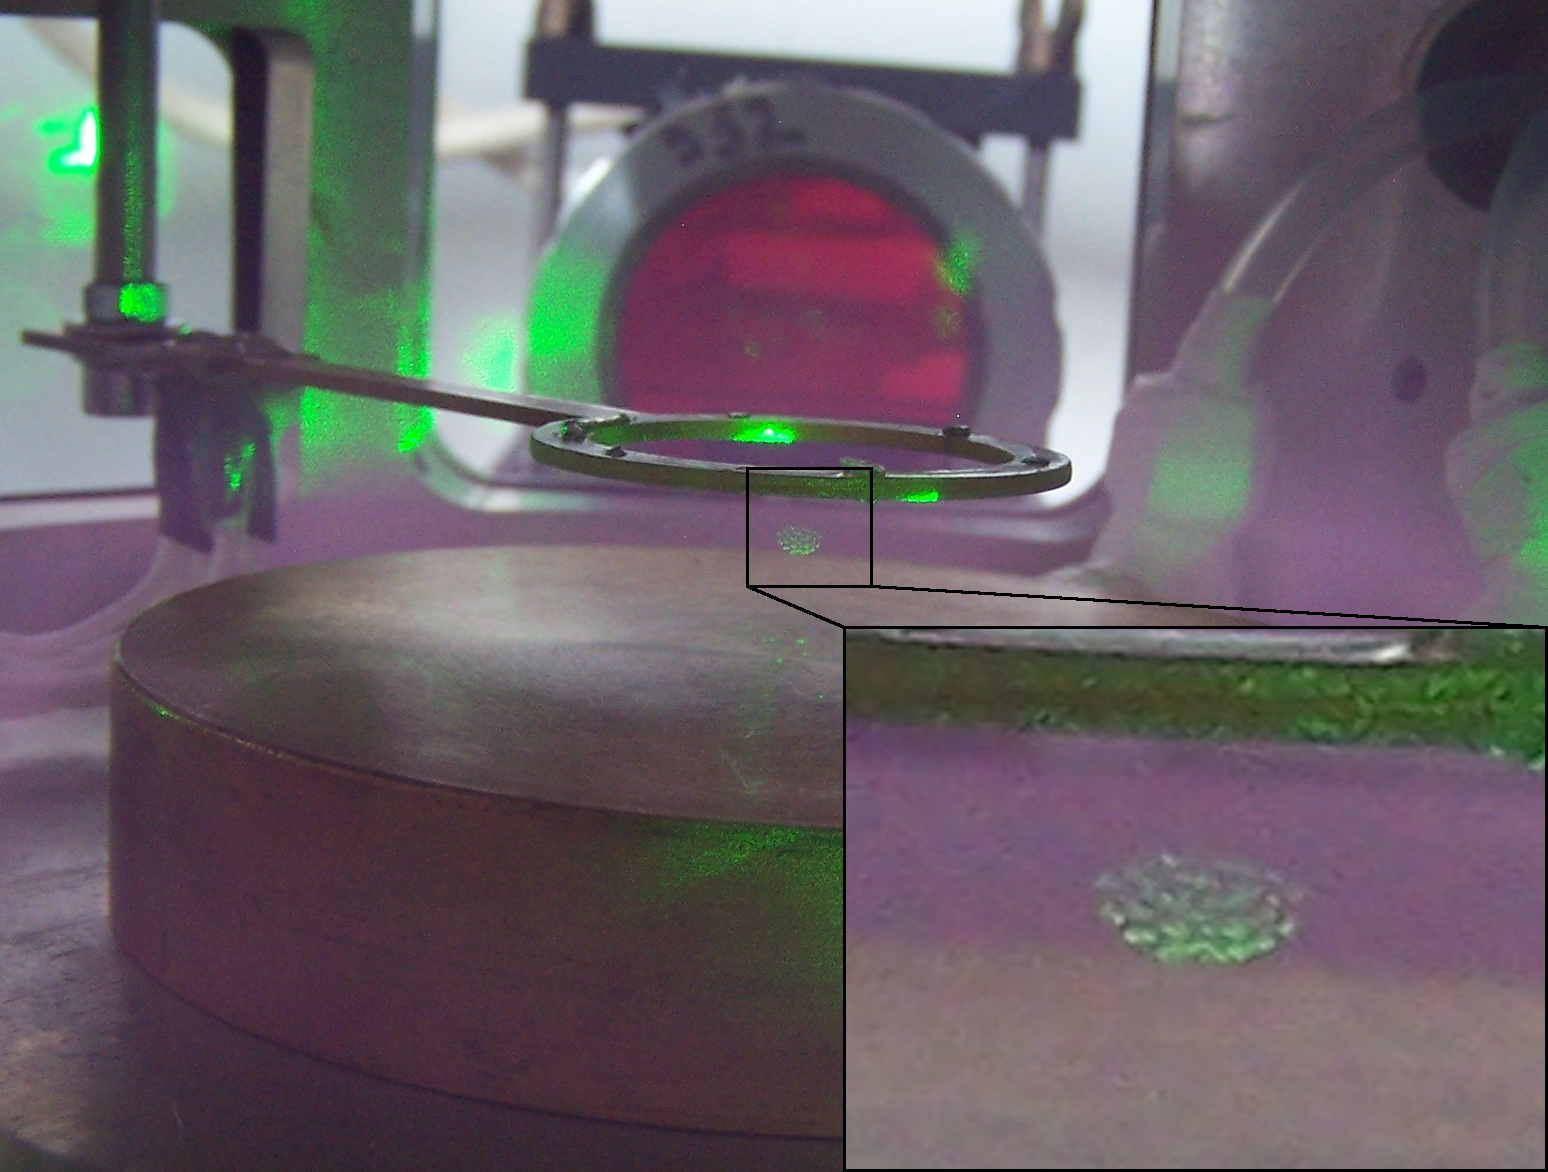
\includegraphics[width=\textwidth,height=0.75\textwidth]{figs/cam/innenansicht.jpg}
						\caption{}
						\label{img:eingefangenerball}
					\end{subfigure}
					\begin{subfigure}[t]{0.48\textwidth}
						\centering
						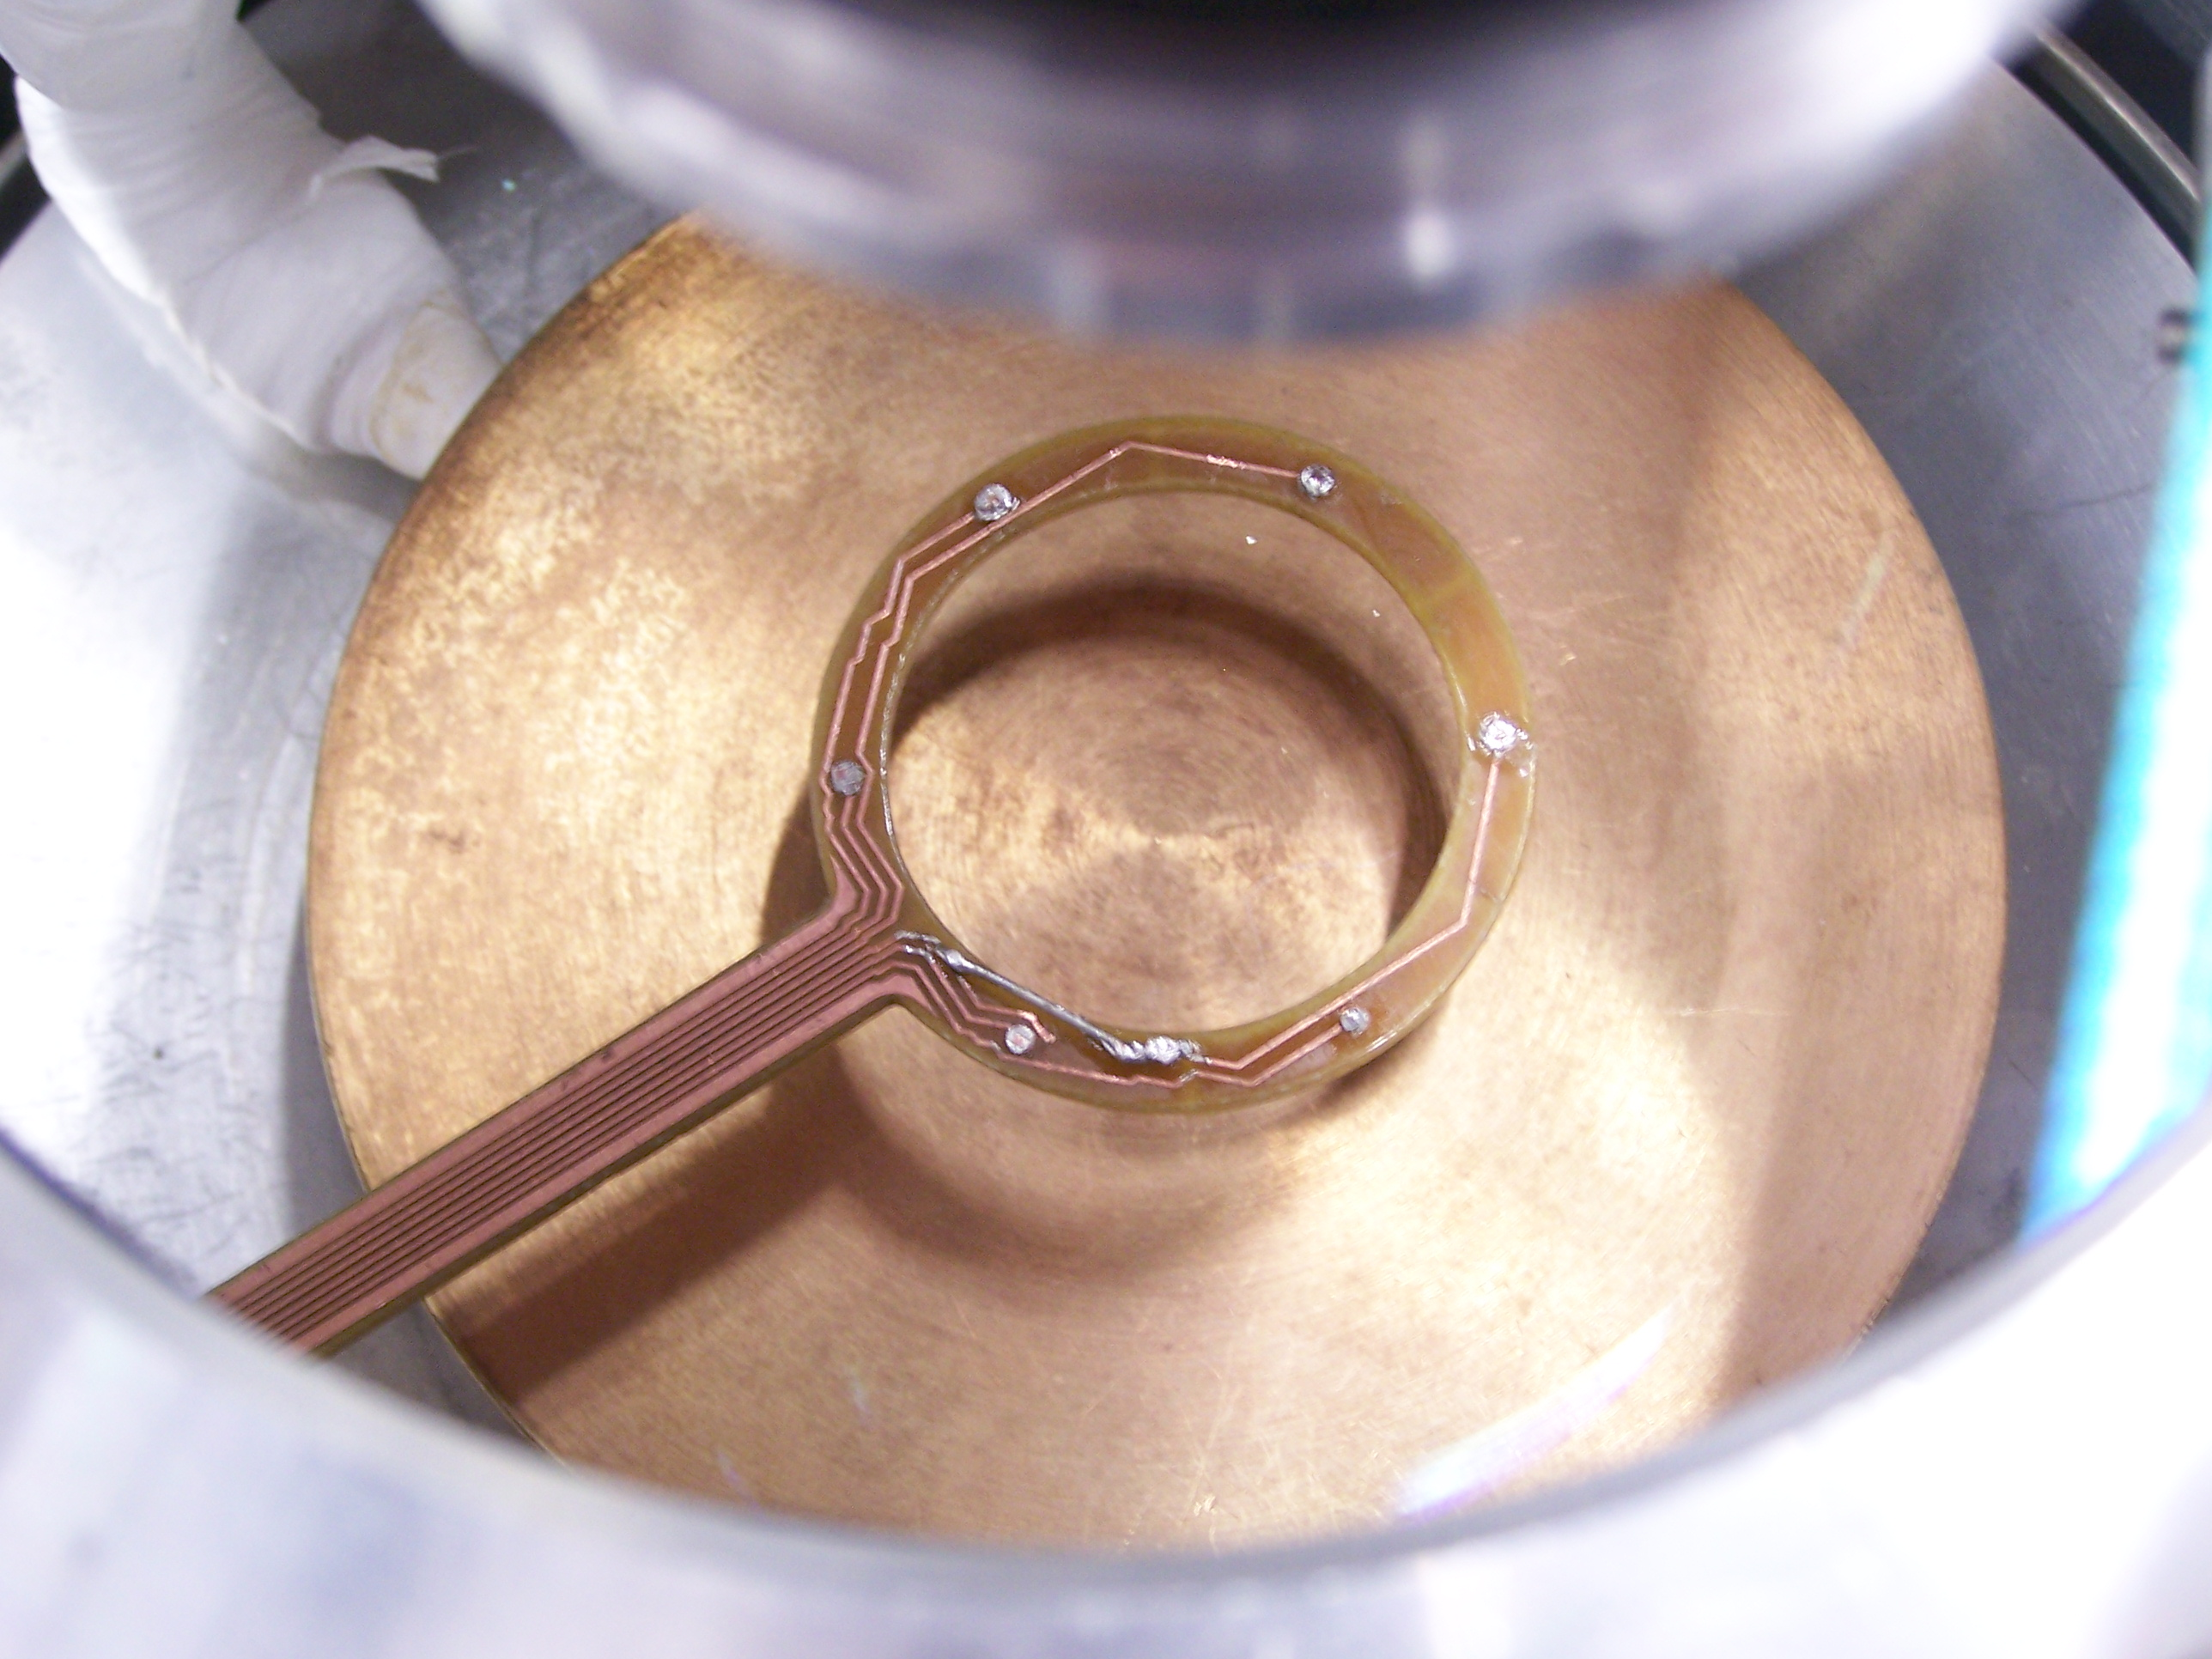
\includegraphics[width=\textwidth,height=0.75\textwidth]{figs/cam/topview.jpg}
						\caption{}
						\label{img:topview}
					\end{subfigure}
					\caption{\fett{(a)}: Einfang eines Yukawa-Balls mit $N\approx40$ unter Beleuchtung mit Nd:YAG-Lasern. Der Cluster befindet sich, leicht abhängig von der Höhe des Rings in der Randschicht, circa $\unit[0,5-1]{cm} $ unterhalb der Elektrode. Im Hintergrund: Kamera 'rot' mit Filter für $\unit[532]{nm}$. \fett{(b)}: Draufsicht durch den Deckel der Kammer auf den Ring. Günstiger Weise befindet sich dieser in der Mitte der Thermophorese, damit aus Sicht des, relativ dazu kleinen Clusters, die Randschicht unendlich ausgedehnt ist.}
				\end{figure}

			Die für den Einfang der Cluster genutzten Segmentringe - wie der in \ref{img:ring} aus Abschnitt \ref{sub:einfang} - sind \"uber Koaxialkabel und eine weitere, unten liegende Vakuum-Durchf\"uhrung (4- bzw. 8-polig) mit der Manipulationselektronik verbunden. Genauer ist damit ein PC mit einer externen \fett{National Instruments 6364}-Karte, welche via USB und das Programm \fett{LabView} angesteuert wird, gemeint. Das erm\"oglicht es, verschiedenste Signale auf die einzelnen Bereiche der Elektrode zu bringen und damit das System gezielt zu heizen bzw. Moden anzuregen (siehe \ref{img:ring}). 

		\subsection{Elektrischer Einfang} \label{sub:einfang}

			Hauptaugenmerk dieses Experiments ist die Manipulation finiter Yukawa-Systeme. Hierf\"ur wurden eigens mehrsegmentige Kupferplatinen konzipiert und konstruiert, siehe \ref{img:ring}. Deren - auf Skalen des Clusters- globaler Einflu{\ss} auf die Randschicht, welchen sie durch ihre zusätzlichen Potentiale erwirken, erm\"oglicht den Einfang eines Staubballs bei niedrigen Gasdr\"ucken und Plasmaleistungen. Weiterhin ist die Geometrie der Ring-Elektrode besonders g\"unstig f\"ur das vorliegende System, da sich somit ein sehr homogenes, sich der Symmetrie des Clusters angepasstes Einfangpotential einstellt.

				\begin{wrapfigure}{r}{0.45\textwidth}
					\centering
					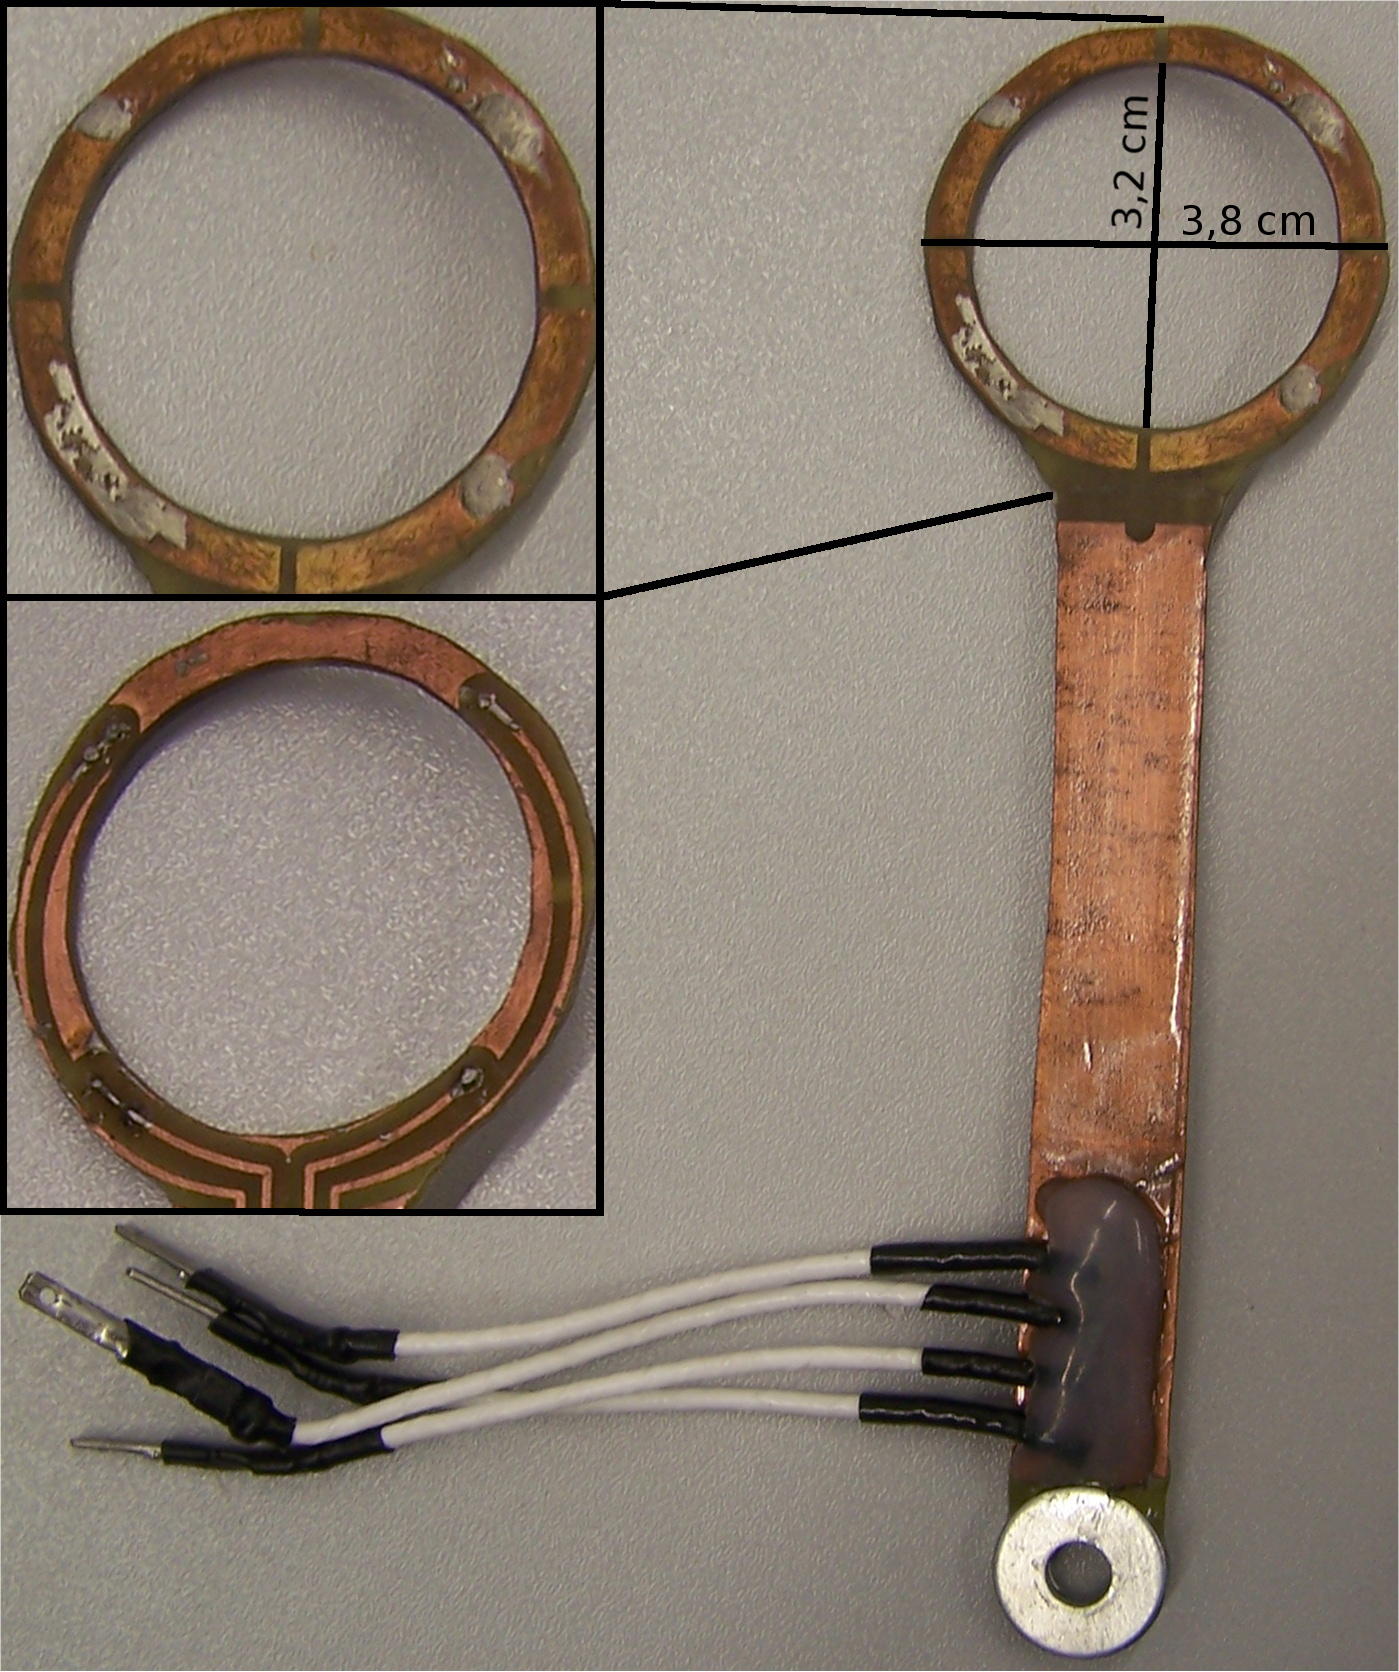
\includegraphics[width=0.4\textwidth,height=0.55\textwidth]{figs/cam/ringelektrode.jpg}
					\caption{Kupferring mit 4 Segmenten \underline{nach} der Benutzung (trotz Plastikumhüllung zeigt der Ring starke Abnutzungen durch Plasma). Am unteren Ende sind die weißen Vakuumkabel zu sehen.}
					\label{img:ring}
				\end{wrapfigure}

			Die verwendeten Ring-Elektroden bestehen aus einem $\unit[6]{mm}$ starken, $\unit[3,2]{cm}$ im Inneren messenden Ring mit 4, 6 oder 8 Segmenten aus Kupfer an der Unterseite, welche später in Richtung des Clusters in der Randschicht zeigen. Dieser Ring ist mit einem Arm, über den die Leiterbahnen der jeweiligen Segmente laufen, verbunden. Am Ende dessen befindet sich eine Bohrung, durch welche die Durchführung mit Schraubgewinde im Kammerdeckel geführt werden kann und somit die Positionierung bei geschlossenem Aufbau ermöglicht. Die gelöteten Kontaktierungen der Vakuumkabel für die Manipulation, von der Ober- auf die Unterseite führend, liegen knapp vor der Bohrung. Für einen Vergleich siehe \ref{img:ring}, sowie  \ref{img:eingefangenerball}  und \ref{img:topview}.\\
			Ziel der Manipulation durch die segmentierte Ring-Elektrode ist es, verschiedene Moden mit unterschiedlichen Symmetrien - Dipol, Quadrupol usw. - gezielt anzuregen und in diese Energie zu bringen. Durch die Modentheorien aus Abschnitt  \ref{sub:yukawaclust} und deren Ausdrücke für die Energie pro Mode $Q_{lm}\left(\omega\right)$ bzw. $S\ix{p}\left(\omega\right)$ kann danach bestimmt werden, inwiefern die Störung erfolgreich war und welche Konsequenz dies nach sich zieht. Auf die Veränderung der Randschicht durch den Ring wird in \ref{sub:glow} eingegangen.


		\subsection{Strereoskopie und Bildrekonstruktion}

			Die Zeitskala der Dynamik der Staubteilchen erlauben eine strereoskopische Untersuchung des Systems. Die Beobachtung erfolgte \"uber 3, zueinander orthogonale High-Speed-CMOS-Kameras mit 60 bzw. $\unit[105]{mm}$ Objektiven. Deren Aufnahmen von bis zu 500 Bildern pro Sekunde ($\unit{fps}$ - \tilt{frames per second}) haben eine maximale Aufl\"osung von $\unit[1280x1024]{px}$. Dabei nimmt die \tilt{fps}-Zahl mit steigender Auflösung ab: je mehr Daten aufgenommen und verarbeitet werden müssen, umso niedriger ist die maximale, verlustfreie Aufnahmerate.\\
			Für die Messreihen wurden jeweils Bilderserien von 10000 \tilt{frames} aufgenommen, wobei die Geschwindigkeit sich dem zu untersuchenden Sachverhalt anpasste. F\"ur eine "`freie"' Aufnahme lag diese bei 100 Bildern pro Sekunde: der Cluster war entweder ungest\"ort oder wurde bei einer festen Anregungsfrequenz manipuliert. Waren Informationen zu bestimmten Phasen gesucht, so wurde dementsprechend die Kamera mit der Anregung gekoppelt und dabei 4 Bilder pro Periode bei einer Frequenz von bis zu $\unit[6,5]{Hz}$ gemacht. \\
			Beleuchtet wurde der Yukawa-Ball mit 2 gr\"unen Nd:YAG-Lasern, welche bei einer Wellenl\"ange von $\unit[532]{nm}$ und mit einer Leistung von $\unit[600]{mW}$ abstrahlten. Über Strahlaufweiter und Spiegel wurden die Laser diagonal durch die Entladung geleitet (siehe \ref{img:eingefangenerball}). Strahlprofil und Strahlungsdruck (siehe \ref{subsub:laser}) sind durch diesen Aufbau so konstruiert, dass sie f\"ur die Dynamik des Clusters unkritisch sind. Jedoch beobachtet man bei an- und ausschalten der Laser eine Verschiebung des Clusters. In \cite{Mulsow13} sind tiefgreifendere Untersuchungen zur Manipulation mit Lasern vorgenommen worden.\\
			Da die Ausdehnung der Partikel weniger als $10\cdot\lambda$ des Laserlichts ist (siehe \cite{Mie08} o. \cite{Hulst81}), kann zur Beschreibung des Streuverhaltens der Staubteilchen die Mie-Streuung herangezogen werden (\cite{Bonitz10}). Nach dieser Theorie ist das vorw\"arts gestreute Licht am intensivsten. Deswegen befinden sich die Kameras auf den gegen\"uberliegenden Seiten der Punkte, an denen das Laserlicht eingestrahlt wird: es resultiert ein kontrastreiches Bild, auf welchem die Partikel gut vor dem dunklen Hintergrund zu sehen sind (siehe \ref{img:rechts} und weitere). Damit einher gehen jedoch auch Probleme, wie zum Beispiel das es zu einer \"Uberbelichtung oder Komplikation bei der Ausrichtung des Systems aus Cluster, Elektrode, Laser und Vakuumkabel kommen kann.

%			Die Bildverarbeitung erfolgte im graustufigen \tilt{bitmap}-Format, kurz \tilt{*.bmp}. Dabei handelt es sich um ein zweidimensionales Rastergrafikformat, bei dem, wie in einer Matrix, einem Pixel die Graustufen-Information mit einem 8-Bit-Wert zugeordnet wird. Das erleichterte u.a. die Verarbeitung in Hinblick auf Intensit\"atsanalysen, wie die Partikelerkennung oder die Auswertung des Plasma-Glow (siehe \ref{sub:glow}).
            
                \begin{figure}
                    \begin{subfigure}[b]{0.4\textwidth}
                        \centering
                        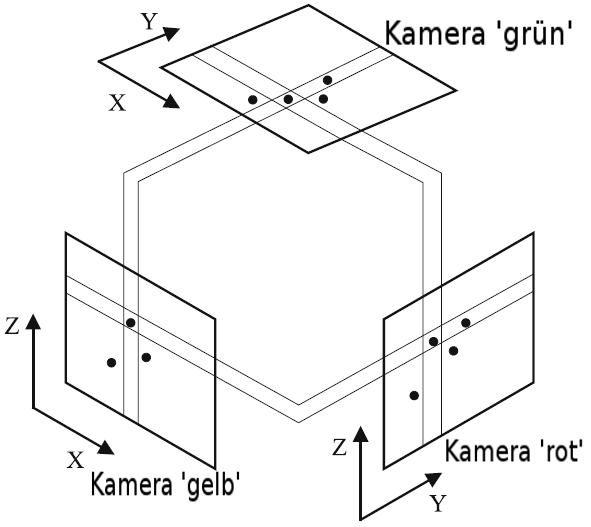
\includegraphics[width=\textwidth,height=5.5cm]{figs/rekonstruktion.png}
                        \caption{}
                    \end{subfigure}
                    \begin{subfigure}[b]{0.56\textwidth}
                        \centering
                        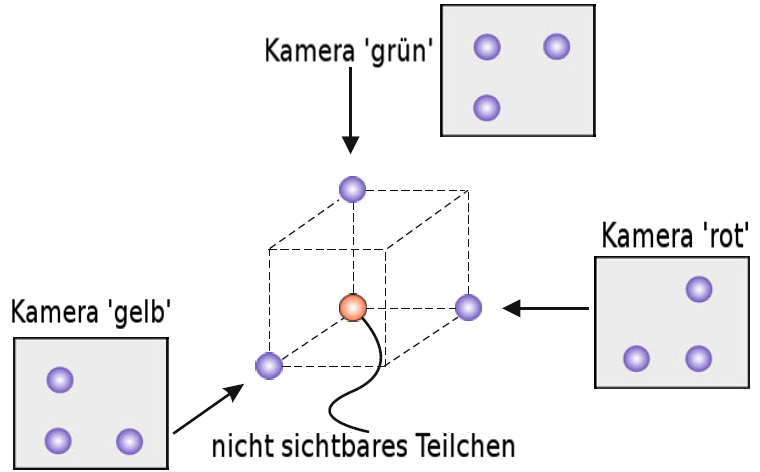
\includegraphics[width=\textwidth,height=5.5cm]{figs/nichtsichtbar.png}
                        \caption{}
                    \end{subfigure}
                    \caption{\fett{(a)}: Rekonstruktion der dreidimensionalen Informationen aus den Bildern der Kameras. \fett{(b)}: Fehler in der Analyse durch Überlagerung von 4 Teilchen in drei Bildern. Für kurze Zeiten des 'Verschwindens' kann mittels Interpolation die Trajektorie des nicht sichtbaren Teilchens vervollständigt werden (nach \cite{Bonitz10}).}
                    \label{img:rekonstruktion}
                \end{figure}

				\subsubsection{3D-Trajektorien}

					Die Rekonstruktion der dreidimensionalen Informationen des Beobachtungsvolumen ist das Kernst\"uck der Stereoskopie (\cite{Bonitz10}). Eingangs m\"ussen aus den einzelnen \tilt{frames} der Kameras die Partikelpositionen gewonnen werden. Daf\"ur analysiert man das Bild durch einen (\tilt{gau{\ss}schen}) Bandpass der Breite des erwarteten Partikeldurchmessers (\cite{Crocker96a}, \cite{Ivanov07}). Au{\ss}erhalb liegende Objekte werden gegl\"attet und angepasst. F\"ur alle erkannten Teilchen wird anschlie{\ss}end, der Intensit\"atsverteilung \"uber diese entsprechend, deren Schwerpunkt ermittelt. Damit erhält man eine Auflösung im Sub-Pixel-Bereich. Es ergeben sich f\"ur alle Kameras die zweidimensionalen Informationen \"uber Partikelpositionen und Clusterausdehnung.\\
					Die Zuordnung der Partikel in gleichzeitigen Kamera-Bildern ist in \ref{img:rekonstruktion}:\fett{(a)} schematisch dargestellt. F\"ur jeden Augenblick der Aufnahme stimmt eine Koordinate der gewonnenen Tupel (eines Partikels) mit einer in den anderen beiden zugeh\"origen \tilt{frames} \"uberein. Dies gilt gerade aufgrund der Orthogonalität des Systems. Durch Abgleich der Informationen von jeweils 2 Kameras und deren Kombination, kann aus den zwei- die dreidimensionalen Koordinaten der Teilchen gewonnen werden. Die letztendlich erhaltenen Partikel-Trajektorien ergeben sich durch die Verknüpfung der \tilt{nearest neighbors} in zwei aufeinander folgenden Bilder. Das heißt, dass die Zusammenführung der Teilchenkoordinaten aus den Aufnahmen zweier Kameras für einen weiteren Zeitschritt fortgesetzt wird. Es wird das Intensitäts-Maximum mit dem kleinsten Abstand zum Ort des betrachteten Partikels im vorherigen Bild gesucht und folglich mit diesem zum entsprechenden Zeitpunkt identifiziert. Die damit erhaltenen Punkte der Bewegung für die diskreten Zeiten der Aufnahme ergeben die Trajektorie.
					Die Rekonstruktion mittels 3 Beobachtungsrichtungen senkt dabei die Wahrscheinlichkeit, dass aufgrund der thermischen Bewegung oder Manipulation (ggf. auch Clusterkonfiguration) Partikel hintereinander verschwinden und somit nicht mehr durchg\"angig aufgenommen werden k\"onnen (siehe \ref{img:rekonstruktion}:\fett{(b)}). F\"ur einzelne Bilder, in denen sich Partikel \"uberdecken, lassen sich jedoch die Trajektorien durch Interpolation, was u.U. f\"ur Fehler in der Auswertung auf Grund von Artefakten sorgen kann, vervollst\"andigen.

		\subsection{Analyse des Plasma-Glow} \label{sub:glow}

			\begin{wrapfigure}{r}{0.5\textwidth}
				\centering
				\vspace{0.25cm}
				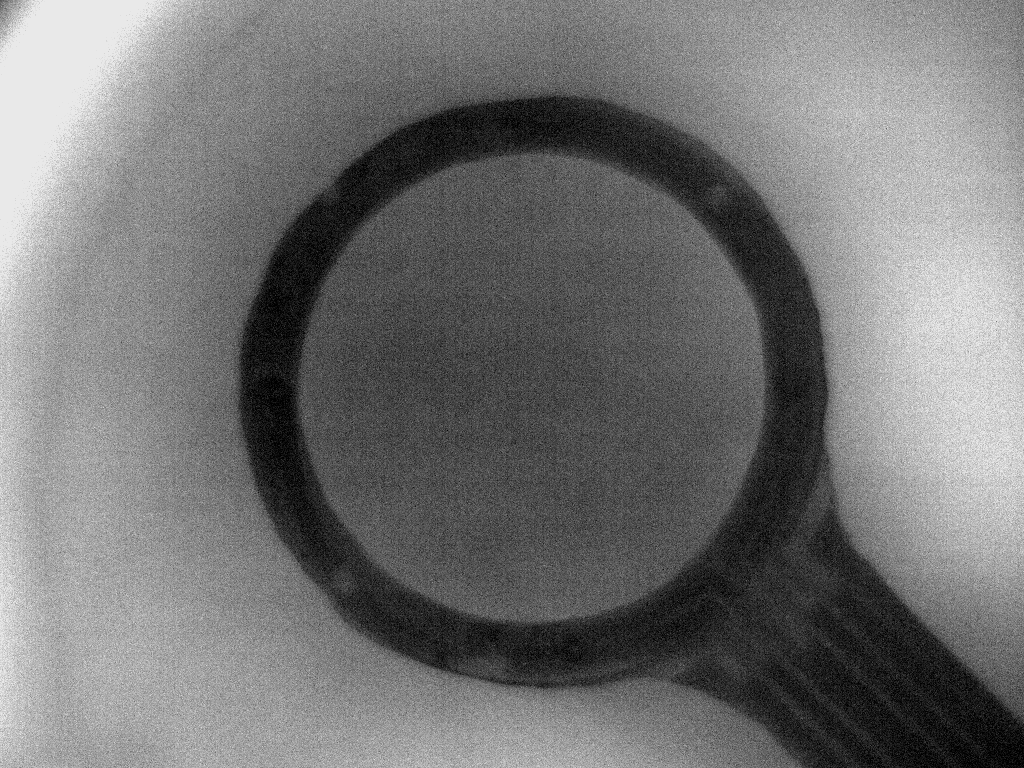
\includegraphics[width=0.45\textwidth,height=0.4\textwidth]{figs/ringplasmglowoben.png}
				\caption{Ein \tilt{frame} ohne Filter für das Licht der Argon-Entladung. Die Helligkeit in der Mitte ist geringer als außerhalb.}
				\label{img:glow}
			\end{wrapfigure}

		Im Zuge der Untersuchung einer Quadrupolschwingung bemerkt man leicht, dass die Teilchen des Clusters, zusätzlich zu ihrer Auslenkung in der Ebene, eine vertikale Schwingung mit Maximum zum Zeitpunkt des Nulldurchgangs der sinusoidalen Signale ausführen. Die Anregung dieser Mode enthält jedoch keine solchen Anteile. Diese Beobachtung legt demnach nahe, dass die Randschichtveränderung durch das Einfangpotential nicht vernachlässigbar für die Kinematik des Cluster ist.\\
		Aus den Abschnitten \ref{sub:kaprfplasm} und \ref{sub:rand} wissen wir,  dass sich beispielsweise um metallische Objekte in einem Plasma eine Grenzschicht ausbildet. Weiterhin ist deren Ausdehnung und Eigenschaften abhängig vom Potential des lokalen Plasmas bzw. des Objektes selbest. Deswegen ist die Manipulation eines Yukawa-Clusters nicht nur als elektrostatische Wechselwirkung Staub und Ring-Elektrode (siehe \ref{img:potential}) zu verstehen, sondern viel mehr als Summe dessen und der Veränderung der lokalen Randschicht, in welcher sich die Staubpartikel befinden. Letztenxdlich war der Einfang eines Staub-Balls als Balance mit der elektrischen Kraft zu verstehen, welche gerade durch das Feld in der Randschicht bei $\unit{\upmu m}$ bestimmt wurde.\\
		Ein Maß für ihre Ausdehnung, und somit daraus folgend ihre weiteren Eigenschaften, ist das Leuchten der Neutralgasatome des Argons. Dieses ist intensiver, je größer die vorliegende Elektronendichte und/oder -temperatur ist (siehe \ref{sub:rand}).  Auf Grund dessen erhält man aus einer Intensitätsanalyse des Bereiches aus \ref{img:glow} Informationen über die Stärke der Randschichtveränderungen.\\
        Ohne die, während der restlichen Messungen an den Kameras angebrachten Filter für das Plasmaleuchten, wurden Aufnahmen für verschiedenste Anregungen gemacht. Das heißt: die 4 Segment des Ringes wurden, entsprechend der gewünschten Symmetrie, mit einer festen Phase zueinander und Frequenz mit einem sinusoidalen Signal der Amplitude $\unit[10]{V}$ beschaltet. Von Interesse sind dabei jedoch nur die Bilder der Oberkamera ('grün', siehe \ref{img:glow}). Die \tilt{bitmaps} werden für die Analyse zuerst auf ein \tilt{range of interest} - ein Kreis bzw. eine Kreisscheibe, in welcher das Leuchten ausgewertet werden soll - beschnitten. Anschließend wird das \tilt{ROI} in Radius- und Winkelabschnitte eingeteilt, welche in ihrer Intensität aufsummiert werden. Ein anschauliches Beispiel für die Darstellung des Intensitätsverlaufs einer Rotationsschwingung, in radialer und polarer Auflösung, wird in \ref{img:glowanalys} gezeigt.

            \begin{figure}[H]
                    \centering
                    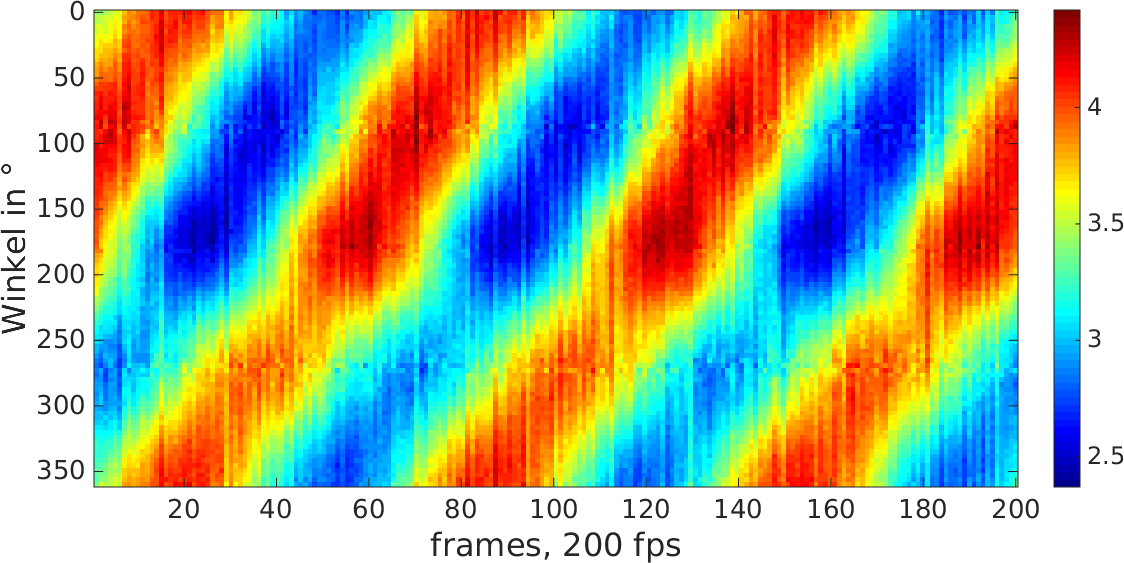
\includegraphics[width=0.8\textwidth,height=0.25\textheight]{figs/glowbeispielrotation3Hzang.png}
            \end{figure}

        \vspace{-0.5cm}

            \begin{figure}[H]
                    \centering
                    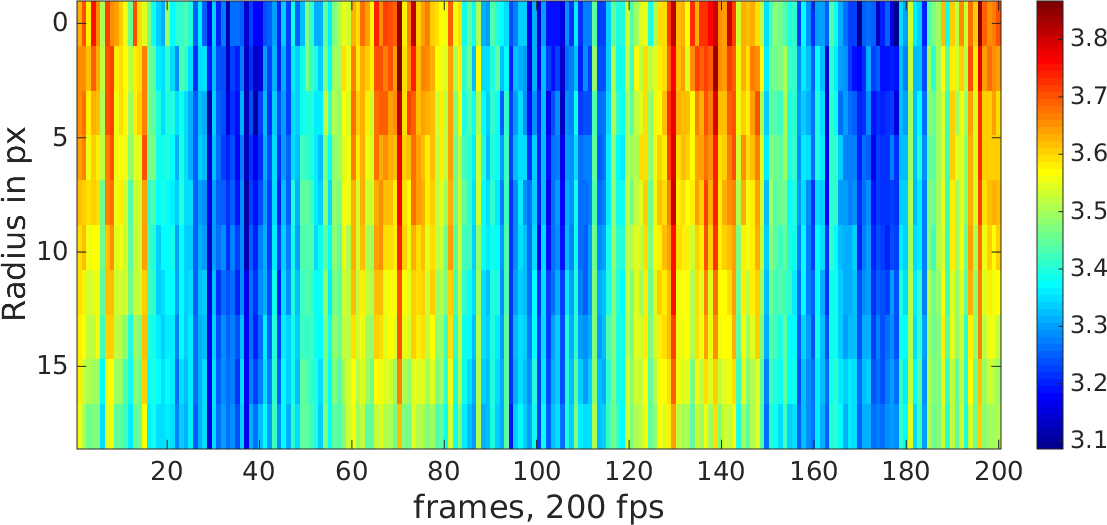
\includegraphics[width=0.8\textwidth,height=0.25\textheight]{figs/glowbeispielrotation3Hzrad.png}
                    \caption{\underline{\fett{oben}}: Winkelaufgelöste Rotationsanregung ($\unit[3]{Hz}$, max. Amplitude). Bei $\unit[250]{\degree}$ ist eine Asymmetrie zu erahnen. \underline{\fett{unten}}: Radiale Auflösung. Die Randschichtveränderung ist innen stärker als außen.}
                    \label{img:glowanalys}
            \end{figure}
            
		\subsection{Phasenaufgelöste Aufnahme}

			Die Anregung über die Ring-Elektrode aus \ref{sub:einfang} ist sinusoidal. Die Kraft durch das zusätzliche Potential hat demnach die Form $F\ix{ext}=K\sin\left(\omega t\right)$, wobei $K$ eine kleine Amplitude ist und $\omega$ die Anregungsfrequenz. Da aus den bisherigen Überlegungen klar ist, dass der Staub-Cluster Reibungskräfte erfährt, lässt sich dessen Schwingungsantwort $C\left(t\right)$ in Hinblick auf die Manipulation als, um den Faktor $\gamma$ gedämpfter, harmonischer Oszillator verstehen, siehe Gl. (\ref{eq:gedämpft}) nach \cite{Carstensen11}. Außerdem ist aus Abschnitt \ref{subsub:moden} bekannt, dass das System ebenso eine Eigenfrequenz $\omega\ix{0}$ besitzt. Diese zu bestimmen ist u.U. sehr aufwändig, muss man doch bei kontinuierlichen Messungen für relativ große Zeiten beobachten, um schließlich für eine einzelne Frequenz die Resonanzantwort zu bestimmen. Geht man hingegen von den Gl. (\ref{eq:gedämpft}) - (\ref{eq:amplitud}) aus, so reicht es, die Amplituden zu 4 verschiedenen Phasen - für $\phi\omega t=0\degree,90\degree,180\degree,270\degree$ verschwindet jeweils ein Teil in Gl. (\ref{eq:gedämpft}) - aufzunehmen, um daraus schließlich $\omega\ix{0}$ zu errechnen.

				\begin{align}
					C\left(t\right)=a\left(\omega\right)\sin\left(\omega t\right)+&b\left(\omega\right)\cos\left(\omega t\right) \label{eq:gedämpft} \\
					a\left(\omega\right)=-\frac{K\left(\omega\ix{0}^2-\omega^2\right)}{\left(\omega\ix{0}^2-\omega^2\right)^2+\left(2\gamma\omega\right)^2} \quad& b\left(\omega\right)=-\frac{2K\gamma\omega}{\left(\omega\ix{0}^2-\omega^2\right)^2+\left(2\gamma\omega\right)^2} \\
					A\left(\omega\right)=\sqrt{a^2\left(\omega\right)+b^2\left(\omega\right)}=&\frac{K}{\sqrt{\left(\omega\ix{0}^2-\omega^2\right)^2+\left(2\gamma\omega\right)^2}} \label{eq:amplitud}
				\end{align}

			Um eine phasenaufgelöste Aufnahme für verschiedene Frequenzen zu machen, wurde die Anregung an die Kameras als neuer Trigger gekoppelt. Das bedeutet, dass die Anregung einen digitalen Puls an die Kameras sendet, wenn sie die entsprechenden Phasen erreicht hat. Für einen Frequenzbereich von $1,6$ bis $\unit[6,5]{Hz}$, bei Inkrementen von $\unit[0,1]{Hz}$, wurden für jeweils 50 Schwingungen 4 Bilder gemacht. Die daraus erhaltenen Daten ergaben Graphen der Art von \ref{img:amplitud}.

				\begin{figure}[H]
					\centering
					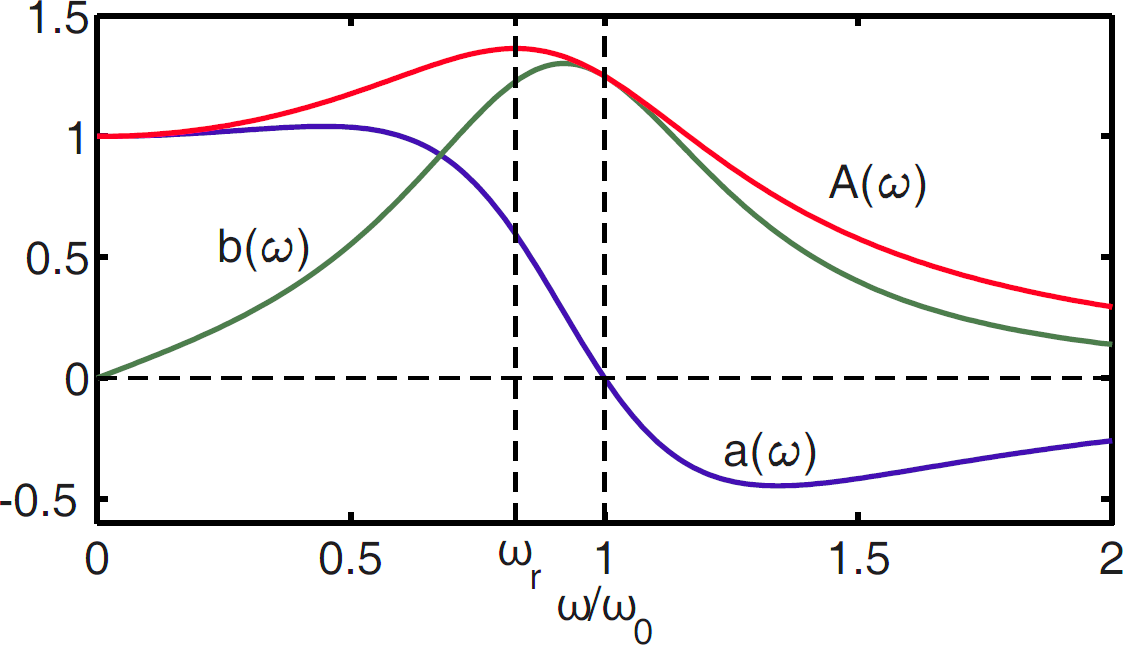
\includegraphics[width=0.7\textwidth,height=0.35\textwidth]{figs/amplitud.png}
					\caption{$A\left(\omega\right), a\left(\omega\right), b\left(\omega\right)$ normiert auf $\omega\ix{0}^2/K $ für $\gamma/\omega\ix{0}=2,5$. Der Wert $\omega\ix{r}$ ist die Resonanzfrequenz, an welcher die Schwingunsantwort die größte Amplitude hat (nach \cite{Carstensen11}).}
					\label{img:amplitud}
				\end{figure}

	\newpage

	\section{Auswertung}\label{sec:auswert}

		In diesem Kapitel werden im Detail die einzelnen Versuche betrachtet und ausgewertet. Dabei wird mit der Analyse des Randschichtverhaltens bei einer Manipulation mit einer 4-Segment-Elektrode begonnen. In den darauf folgenden Abschnitten zur Auswertung der Cluster-Dynamik und dessen Moden werden insbesondere diese Ergebnisse herangezogen.

        \subsection{Untersuchungen der Randschicht}\label{sub:glowanalys}

                \begin{wrapfigure}{r}{0.4\textwidth}
                    \centering
                    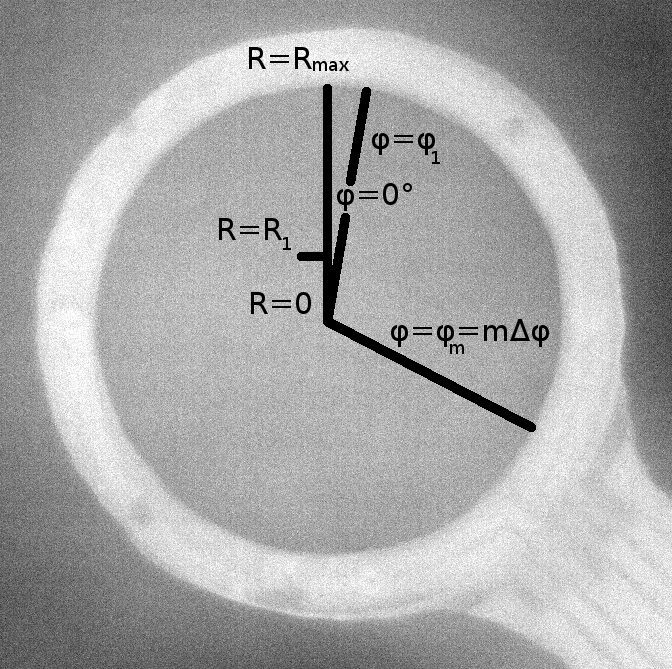
\includegraphics[width=0.4\textwidth,height=0.4\textwidth]{figs/auswertung/plasmaglw/randanalysemaske.png}
                    \caption{Schema der Maske für die Auswertung des Randschicht-Leuchtens (invertiert).}
                    \label{img:randmaske}
                \end{wrapfigure}

		Wie bereits erwähnt, erfolgte die Analyse des Plasma-Glow über die Aufsummierung der Intensitäten in einem selbst gewählten Bildbereich, welcher beliebig polar und radial unterteilt werden konnte. Aus dieser Summe wurde anschließend der Mittelwert der Intensität durch Division der Anzahl an Pixeln, mit einer Helligkeit $>0$ in dem jeweiligen Bereich, berechnet. \ref{img:randmaske} zeigt, schematisch, die erstellte Maske für eine solche Auswertung. Der maximale Radius $R\ix{max}$ sollte dabei, günstiger Weise, immer noch vollständig innerhalb des Ringes liegen, damit keine falschen Helligkeitsinformationen hinzugezogen werden. Die Bildverarbeitung erfolgte nicht, wie es \ref{img:glow} zeigt, sondern im invertieren Zustand. Dies hat zur Folge, das geringe Kontraständerungen als große Differenzen in den Intensitätswerten aufgenommen werden können. \\
		Insgesamt wurden 13 Messreihen von 2000 \tilt{frames} bei einer Bildrate von 200 \tilt{fps} aufgenommen, was demnach einer Messzeit von $\unit[10]{s}$ gleich kommt. Begonnen wurde mit einer ungestörten Messung: das heißt bei einer abgeschalteten Anregung. Dazu kommen jeweils Aufnahmen von Anregungen einer Dipol-, Quadrupol- und Rotationsschwingung bei 3 sowie  $\unit[10]{Hz}$. Diese insgesamt 6 Messungen mit Anregung wurden danach, um noch genauer den Einfluss der Manipulation zu verstehen, für eine niedrigere Ring-Höhe (über der Thermophorese-Zelle) wiederholt. Zuerst betrug diese $\unit[1,8]{cm}$, dann $\unit[1,2]{cm}$. Die Aufnahmen wurden alle bei einem Gasdruck von $\unit[10,6]{Pa}$ und einer \tilt{rf}-Generator-Leistung von $\unit[1,6]{W}$ gemacht. Der relativ hohe Wert - bei Untersuchungen von Staub-Clustern lag dieser nur bei $\unit[0,5]{W}$ - wurde bewusst gewählt, da bei größeren Leistungen das Leuchten ebenso stärker wird. Dies ist u.a. eine Folge der erhöhten Elektronendichten. \\
		Es schließt sich die Beschreibung einer Auswahl der einsichtigsten und am besten nachvollziehbaren Messdaten an. 

			\subsubsection{Messwerte}

					\begin{figure}[!t]
						\centering
						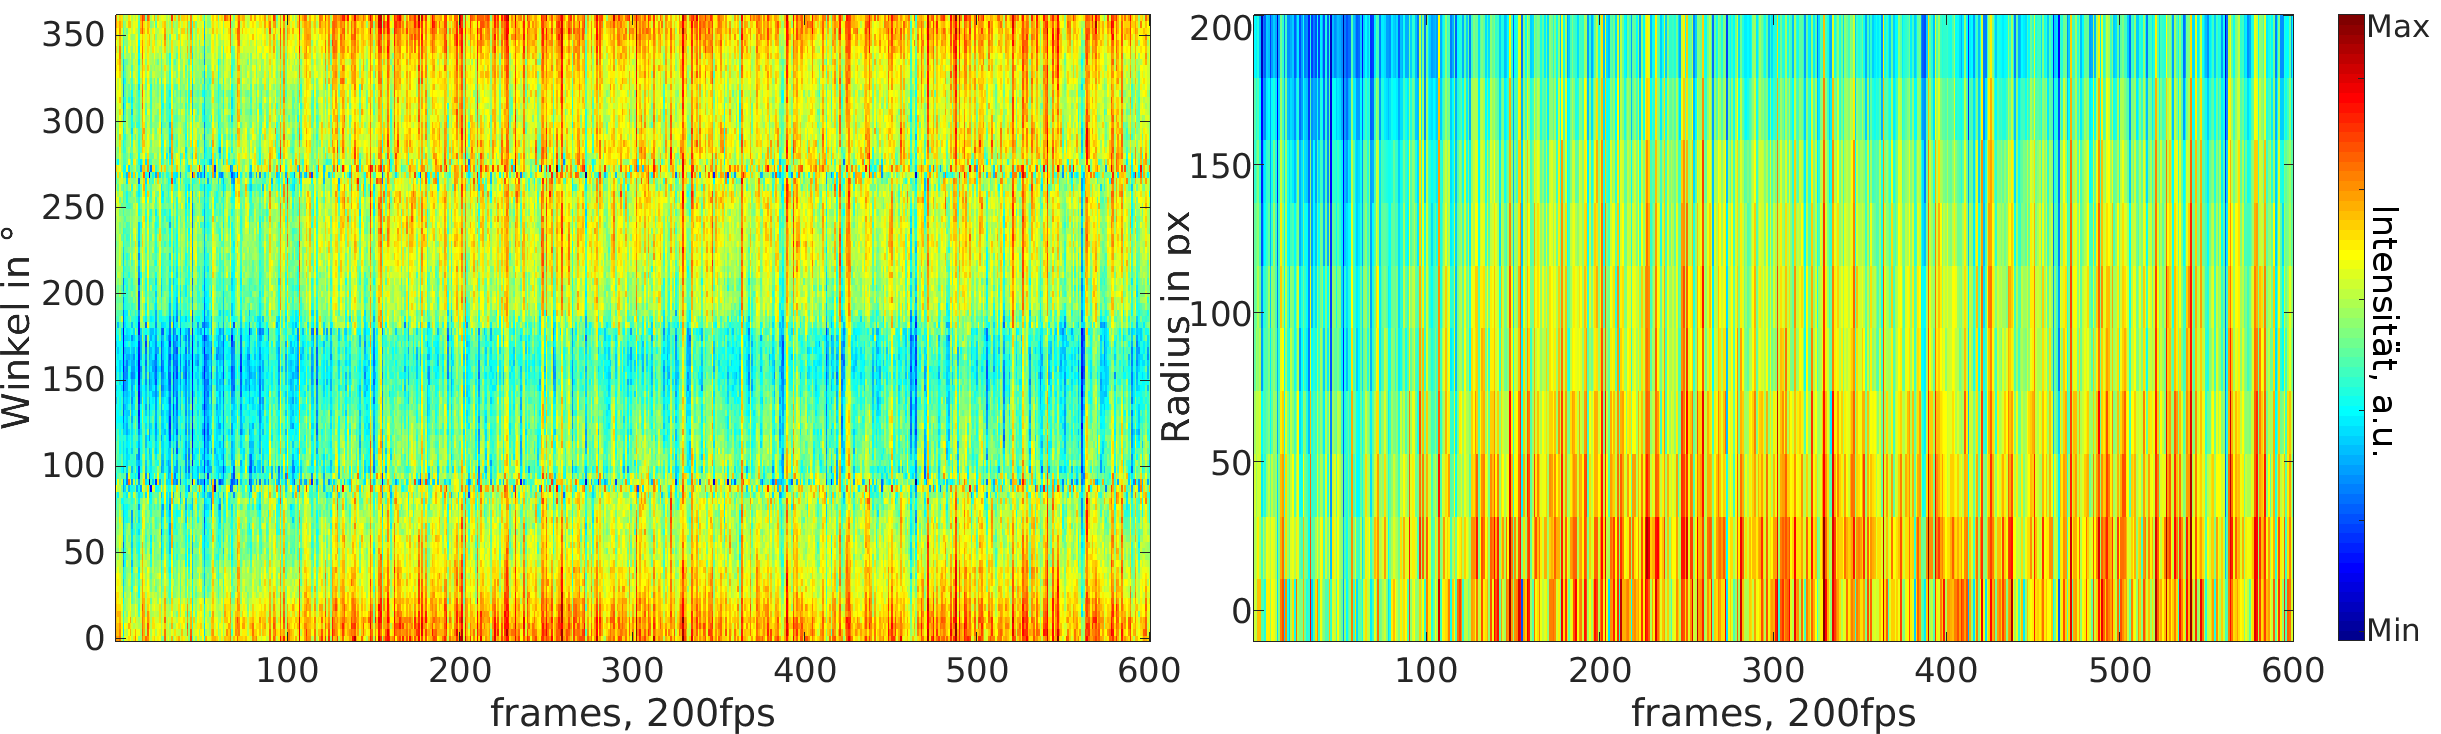
\includegraphics[width=\textwidth,,height=0.38\textwidth]{figs/auswertung/plasmaglw/randungest3sekwinkurad.png}
						\caption{\underline{\fett{links}:} Polar aufgelöster Intensitätsverlauf für eine Zeit von $\unit[3]{s}$ (600 \tilt{frames}) ohne Anregung. Die Intensität (siehe rechts) ist auf einen Durchschnittswert normiert. \underline{\fett{rechts}:} Die selbe Messung wie \underline{\fett{links}}, nur radial aufgelöst. }
						\label{img:randungest}
					\end{figure}

			In \ref{img:randungest} sind die Daten der ersten Messung, in radialer und polarer (Winkel-) Auflösung, bei abgeschalteter Anregung und "`hoher"' Elektrode dargestellt. Zuerst fällt der Intensitätsabfall in der Winkeldarstellung bei $\varphi\approx\unit[140-180]{\degree}$ auf: dieser Bereich entspricht, nach \ref{img:randmaske}, in etwa der Richtung des Arm der Elektrode. Dort ist das Plasma-Leuchten schwächer als am übrigen Ring. Hinzu kommt ein Helligkeits-Gradient von eben diesem Bereich in Richtung $\unit[0/360]{\degree}$. Das entspricht der gegenüberliegenden Seite des Rings. In radialer Darstellung zeigt sich, dass im Inneren der Elektrode, im Vergleich zu Außen, die Intensität wesentlich größer ist.\\
			Die \ref{img:randfrequenz} stellt eine Dipol-Anregung bei den 2 unterschiedlichen Frequenzen dar (s.o.).  Sehr anschaulich und gut erkennbar sind die, sich abwechselnden, Maxi- und Minima der Intensität, welche mit der Frequenz der Anregung für einen Winkel (bspw. $\varphi=\unit[150]{\degree}$) "`durchschwingen"'. Im Bereich $\unit[50-220]{\degree}$ sind die Extrema sehr gut ausgeprägt, wohin gegen um $\unit[330]{\degree}$ der Kontrast zwischen den Schwingungszuständen sich weniger stark abzeichnet. Für eine höhere Frequenz der Manipulation verändert sich, bis auf die Zeitskalen der Variation der Helligkeiten, nichts.

				\begin{figure}[!b]
			       	\centering
			       	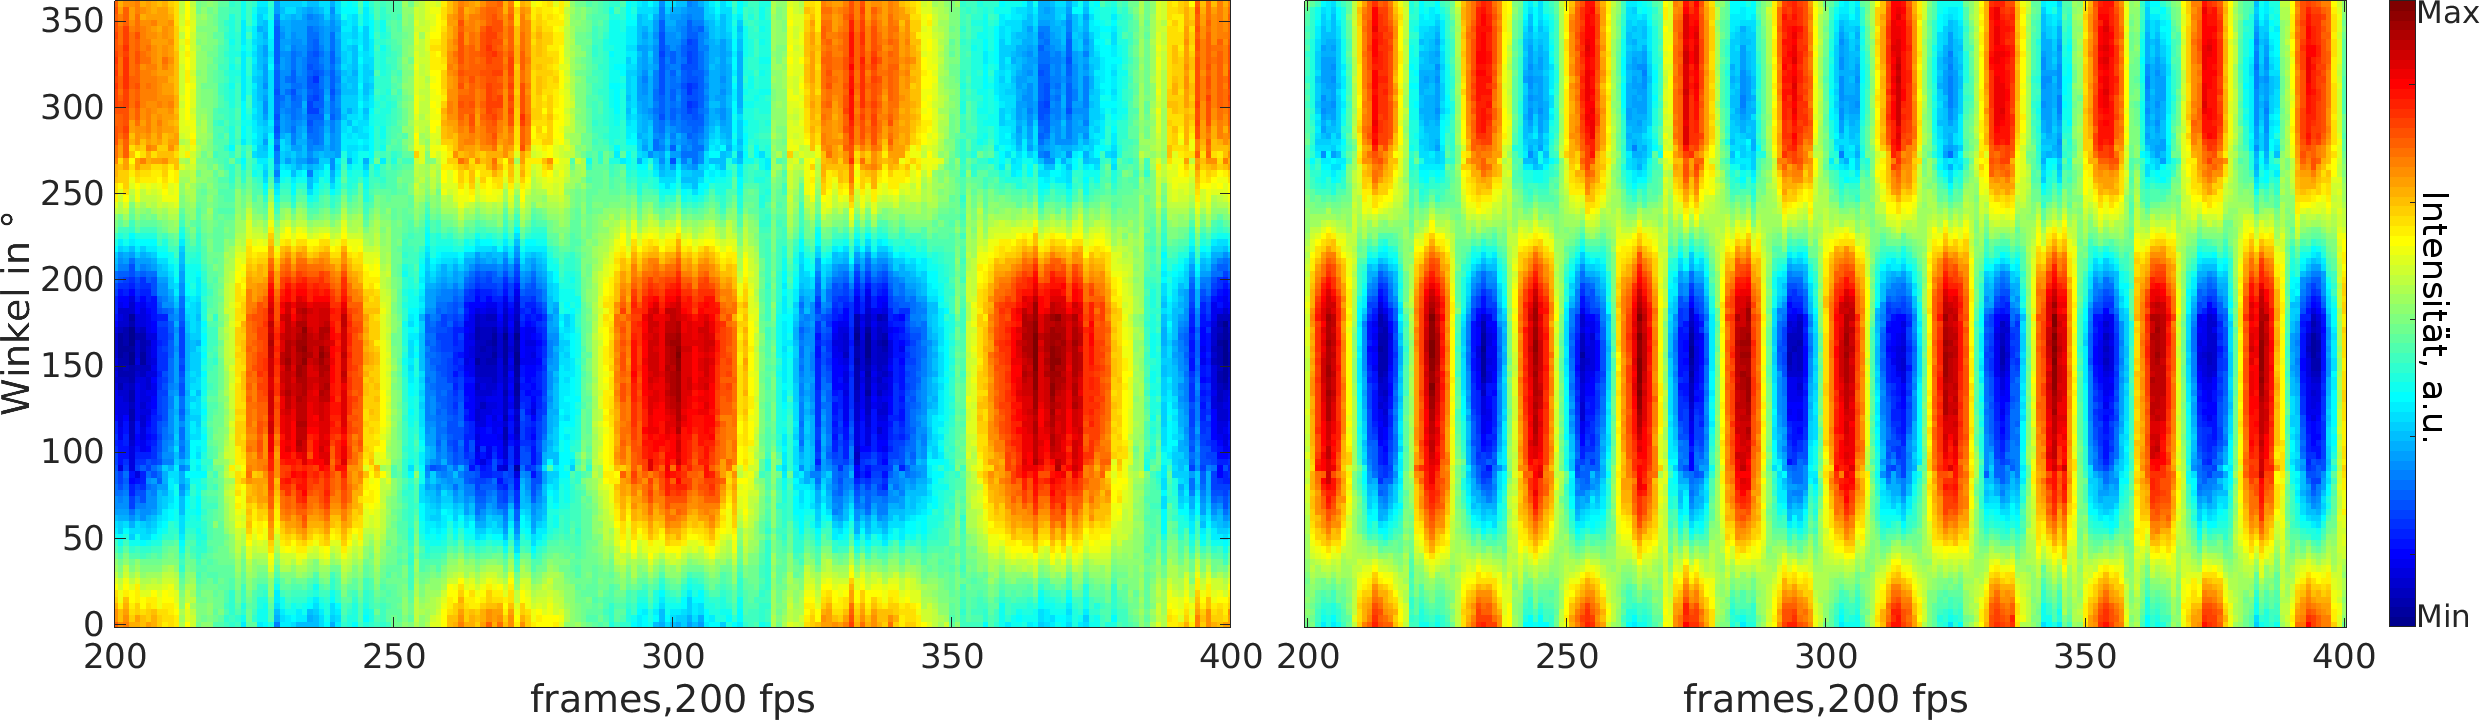
\includegraphics[width=\textwidth,height=0.38\textwidth]{figs/auswertung/plasmaglw/randdipol3hzu10Hz1sekwink.png}
			       	\caption{\underline{\fett{links}:} Winkeldarstellung der Dipol-Anregung bei $\unit[3]{Hz}$ für $\unit[1]{s}$. \underline{\fett{rechts}:} Bei $\unit[10]{Hz}$.}
			       	\label{img:randfrequenz}
				\end{figure}

				\begin{figure}[!t]
					 \centering
					 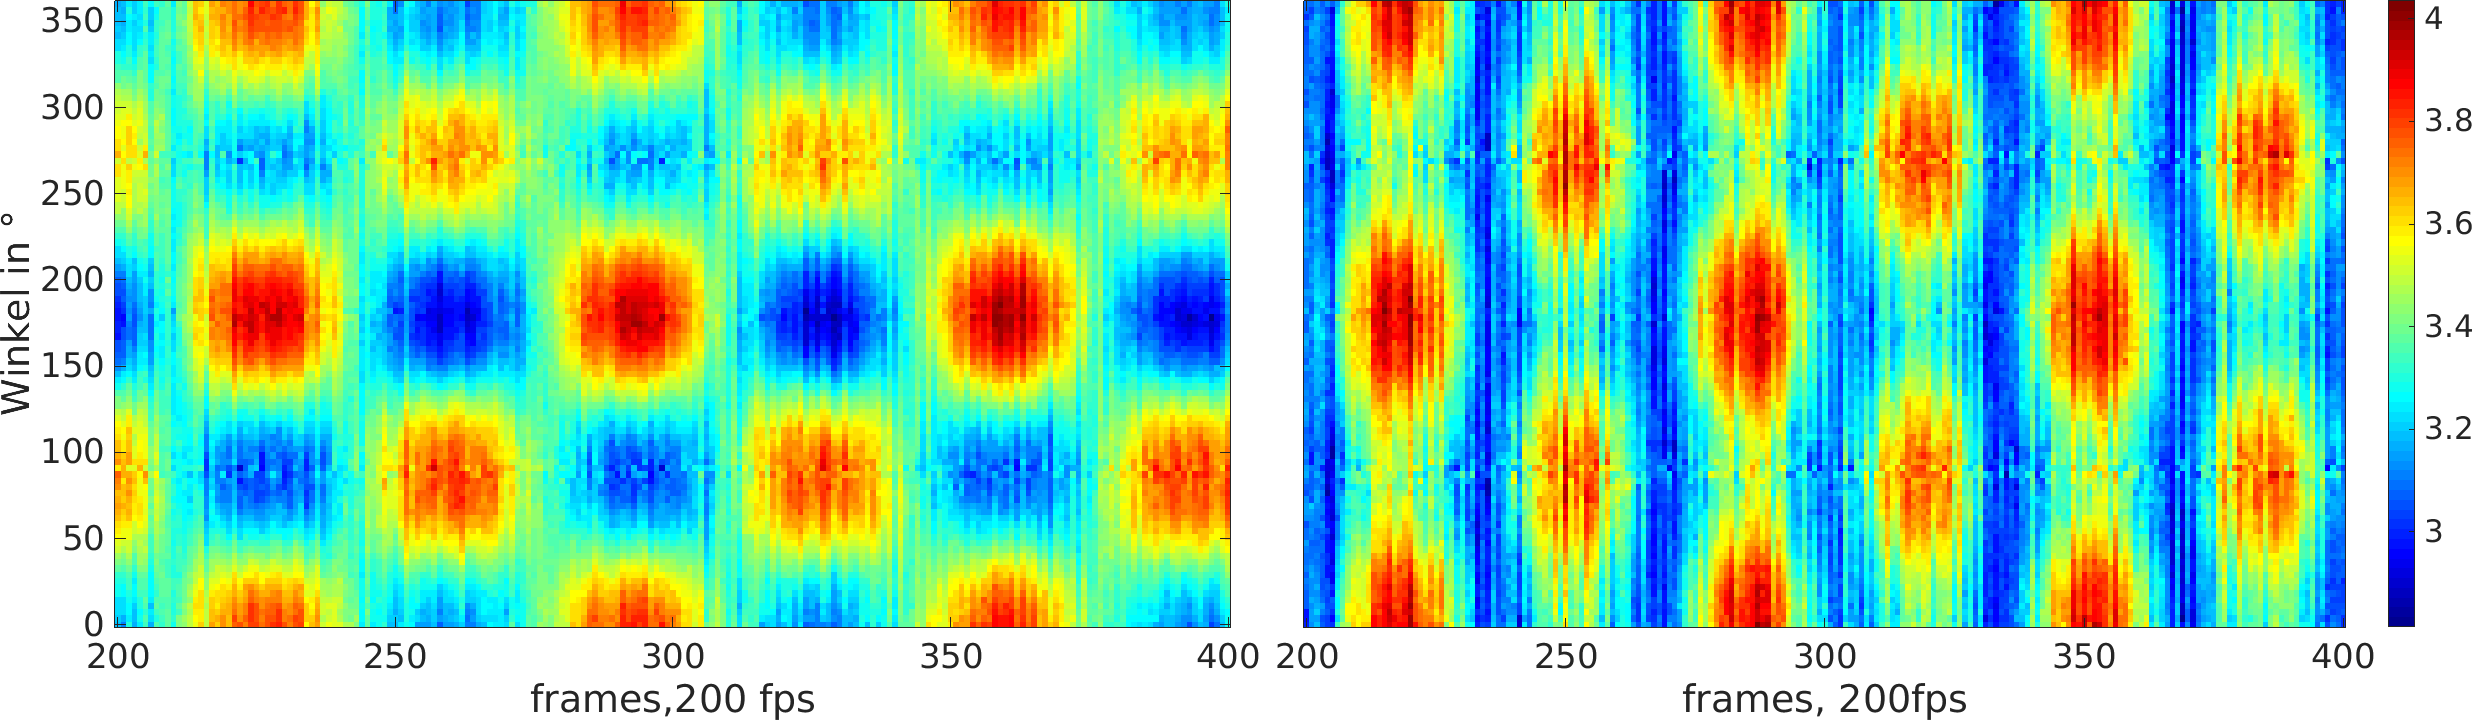
\includegraphics[width=\textwidth,,height=0.38\textwidth]{figs/auswertung/plasmaglw/randhochutiefquad3Hz1sekwink.png}
					 \caption{Winkelaufgelöste Quadrupol-Anregung bei $\unit[3]{Hz}$. \underline{\fett{links}:} für eine Höhe von $\unit[1,8]{cm}$. \underline{\fett{rechts}:} Für $\unit[1,2]{cm}$.}
					 \label{img:randhochutiefwink}
				\end{figure}

	        In \ref{img:randhochutiefwink} ist der Unterschied für die unterschiedlichen Höhen der Elektrode an einer Quadrupol-Anregung mit $\unit[3]{Hz}$ gezeigt. Bei einer Höhe von $\unit[1,8]{cm}$ (\ref{img:randhochutiefwink}:\underline{\fett{links}}) fällt einerseits eine Asymmetrie zwischen den Maxima bzw. Minima einer Schwingungsachse auf. Jeweils 2, für einen Zeitschritt wie etwa für die \tilt{frames} 250 bis 275 zusammen auftretende, Extrema gehören zu einer Anregungsrichtung: zwischen $\unit[0/360]{\degree}$ und $\unit[180]{\degree}$, hier einmal $\Pi$ genannt, sowie $\unit[90]{\degree}$ und $\unit[270]{\degree}$, als $\Sigma$ bezeichnet. Andererseits - und dieser Unterschied ist wesentlich signifikanter - sind die Differenzen zwischen den Maxima und Minima der beiden Achsen. Die größten Intensitäten der Schwingungsrichtung $\Pi$ sind deutlich höher, als die der Achse $\Sigma$. Außerdem sind die Minima auf $\Sigma$ niedriger, als auf $\Pi$. In der Zeit, in welcher keiner der 4 Segmente eine Amplitude (max. oder min.) der Anregung trägt, zeichnet sich ein Übergang von einem Extremum zum anderen ab. Beispielsweise für die \tilt{frames} 335 bis 345 stellt sich im gesamten Ringbereich eine,näherungsweise gleiche Helligkeit ein.

				\begin{figure}[!b]
					\centering
					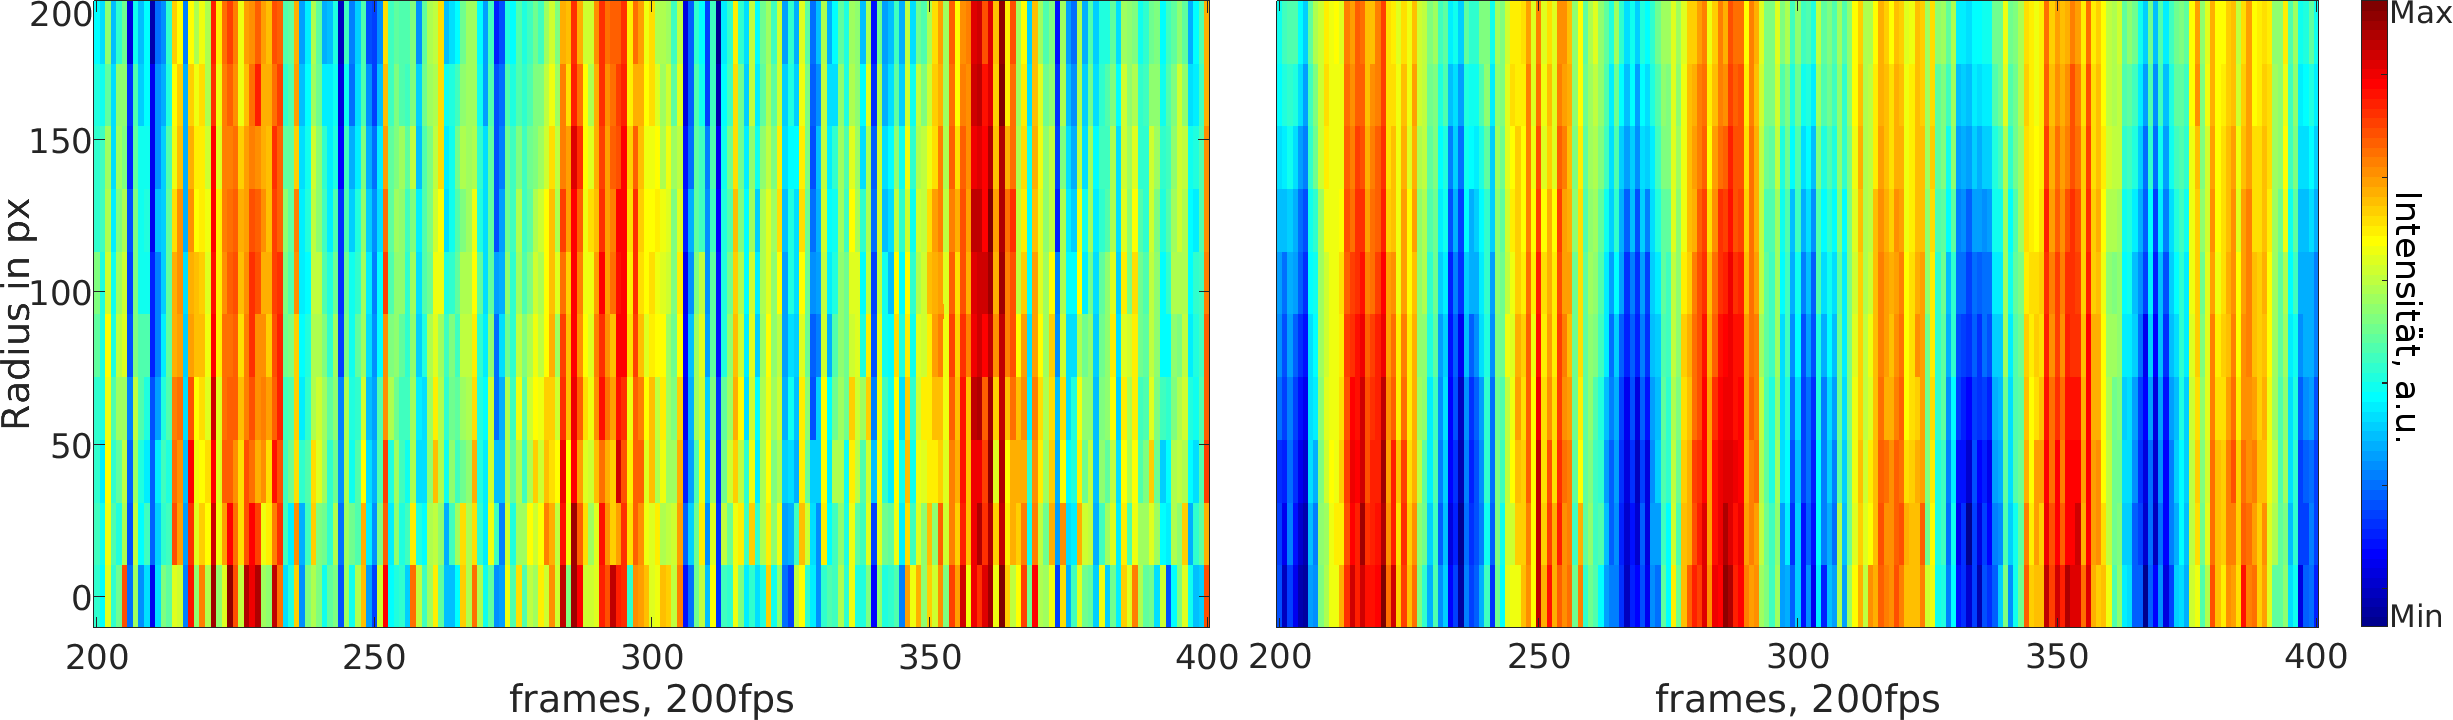
\includegraphics[width=\textwidth,height=0.38\textwidth]{figs/auswertung/plasmaglw/randhochutiefquad3Hz1sekrad.png}
					\caption{Radial aufgelöste Quadrupol-Anregung (selbige wie in \ref{img:randhochutiefwink}) bei $\unit[3]{Hz}$. \underline{\fett{links}:} für eine Höhe von $\unit[1,8]{cm}$. \underline{\fett{rechts}:} Für $\unit[1,2]{cm}$.}
					\label{img:randhochutiefrad}
				\end{figure}

			Für eine niedriger angebrachte Elektrode (\ref{img:randhochutiefwink}:\underline{\fett{rechts}}) findet man in etwa den gleichen Intensitätsverlauf wie zuvor. Es fallen Unterschiede sowohl zwischen den Maxima und Minima auf einer Schwingungsachse, als auch im Vergleich der beiden auf. Jedoch erkennt man weiterhin, im Kontrast zur Aufnahme bei einer hohen Elektrode, dass diese weniger scharf abgezeichnet sind. Das heißt: die Grenzen bzw. Übergänge der Extrema zwischen $\Sigma$ und $\Pi$ haben einen geringeren Intensitäts-Gradienten. Besonders gut ist dies im Bereich um \tilt{frame} 250 (und 100 \tilt{frames}-periodisch fortlaufend) zu erkennen - die Maxima dieser Phase der Anregung sind sehr verwaschen und verlaufen sich über den gesamten Winkelbereich. Jedoch zeichnet sich in den Momenten zwischen den Amplituden ein klares Tief in der Intensität ab, welches die Extrema unterschiedlicher Phasen der Anregung voneinander trennt. Für das Beispiel bei  \tilt{frame} 250 liegen diese zwischen \tilt{frame} 230 und 245, sowie 255 und 225. Demnach kann der Umschicht-Vorgang, welcher in \ref{img:randhochutiefwink}:\underline{\fett{links}} als heller Übergang zwischen den Maxima der Achsen zu erkennen ist, im zeitlichen Verlauf nicht beobachtet werden. Lediglich gewinnen die Maxima auf $\Sigma$ geringfügig an Intensität, wohin gegen die Minima sowohl auf $\Sigma$ als auch $\Pi$ weniger ausgebildet sind.\\
			Die \ref{img:randhochutiefrad} zeigt die exakt gleiche Messung wie die vorherige aus \ref{img:randhochutiefwink}, nur in radialer Auflösung. Das linke Bild zeigt die Daten aus der Messung bei einer höheren Elektrode. Für die Zeiten um die \tilt{frames} 225, 290 und 360 ist jeweils das gesamte Innere des Ringes hell. Das heißt, dass über den gesamten radialen Bereich ein Maximum zu finden ist. Zwischen diesen können weitere erahnt werden. Jedoch sind diese Extrema, sowohl die maximalen als auch minimalen, sehr flach bzw. kaum erkennbar. Sie heben sich lediglich auf Grund der kleinen Bereiche um \tilt{frame} 210, 245, 275 310, 340 und 375 bei großen Radien, wie etwa $\unit[150-200]{px}$, von den übrigen Intensitäts-Maxima ab. Weiterhin ist insgesamt ein schwacher Gradient in der Helligkeit von innen $R=0$ bis $R=\unit[200]{px}$ zu erkennen.\\
			Bei einer tiefen Elektrode zeigt sich ein anderes Bild: alle Extrema sind scharf und eindeutig erkennbar. Für diese Einstellung zeigt sich die zuletzt benannte Diskrepanz zwischen den Schwingungsachsen nun wesentlich deutlicher. Demnach können die Schwingungen aus der vorherigen Beschreibung mit denen dieser Darstellung identifiziert werden. Das 1. Maximum gehört zu $\Pi$ und das 2. zu $\Sigma$ usw. Außerdem stellt man fest, dass die Helligkeit der Maxima von $\Sigma$ geringer ist, als die von $\Pi$. Interessant ist hingegen jedoch, dass die minimalen Intensitäten keine systematischen Differenzen mehr zueinander aufweisen. Für große Radien verschwimmen die Intensitäten und der Gradient nimmt, in Hinblick auf $R=0$, mit wachsendem Abstand zum Mittelpunkt zwischen den Extrema ab.

				\begin{figure}[!t]
					\centering\vspace{-0.5cm}
					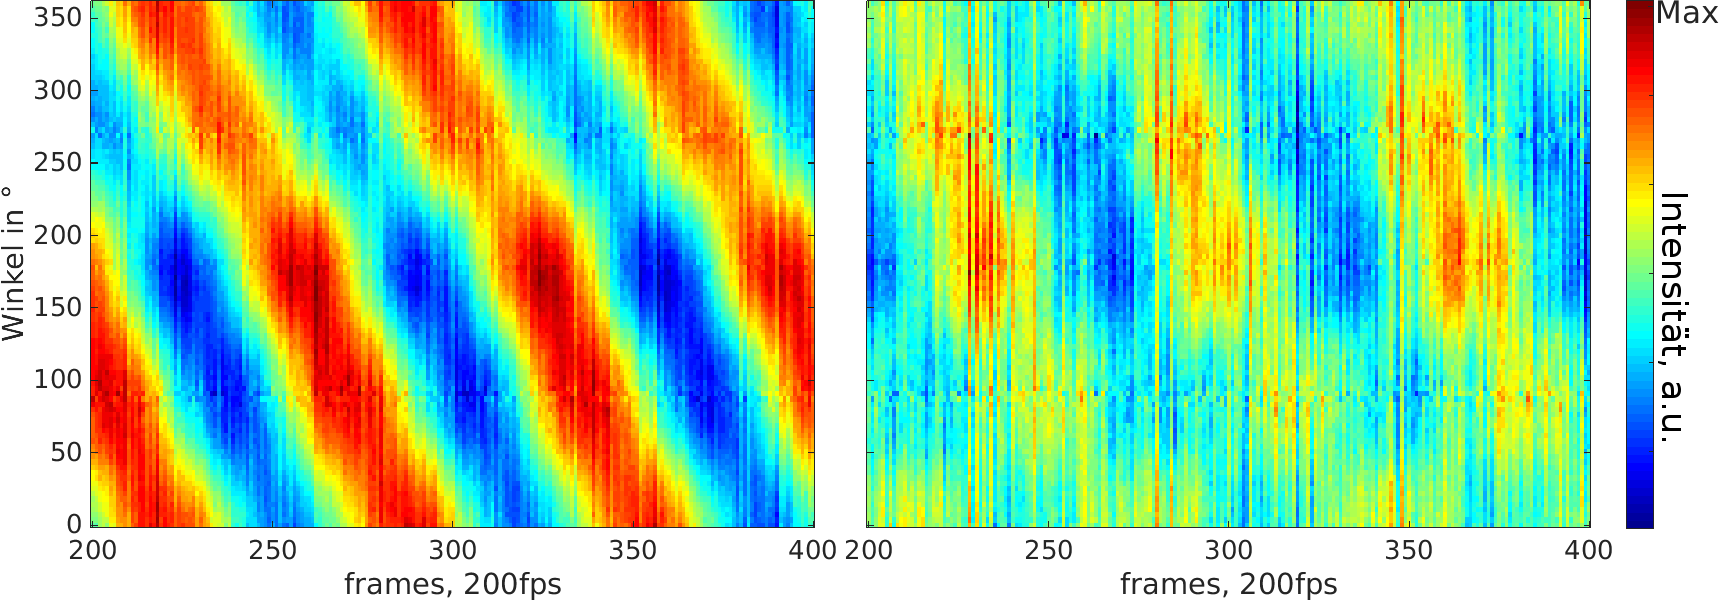
\includegraphics[width=\textwidth]{figs/auswertung/plasmaglw/randrotathochutief3Hz1sekwink.png}
					\caption{Intensitätsverlauf der Anregung einer Rotation bei $\unit[3]{Hz}$ und einer Zeit von $\unit[1]{s}$. \underline{\fett{links}:} Hohe Elektrode. \underline{\fett{rechts}:} Tief.}
					\label{img:randhochutiefrotat}
				\end{figure}

			Abschließend ist in \ref{img:randhochutiefrotat} eine Rotations-Anregung mit Hilfe der Intensitätsanalyse visualisiert. Sehr anschaulich kann hier das Maximum bei seiner Wanderung von $\unit[360]{\degree}$, im Bereich um \tilt{frame} 235 (und um $200/3$ \tilt{frames} fortsetzend), über $\unit[180]{\degree}$ bei ca. \tilt{frame} 260 , bis hin zu $\unit[0]{\degree}$ bei \tilt{frame} 300 verfolgt werden. Im Zuge dessen können über das gesamte Winkelintervall mehr oder weniger stark ausgeprägte Inhomogenitäten der Intensität beobachtet werden: insbesondere bei $\unit[240-250]{\degree}$ ist ein stärkerer Abfall in der Helligkeit des Maximums zu vermerken. Um $\unit[180]{\degree}$ liegt die größte Intensität. Das Minimum zwischen den Bahnen der Rotationsanregung ist, bis auf eine Aufhellung und ein "`Verschmieren"' im Bereich des schwachen Maximums, gleichbleibend.\\
			Das rechte Bild der \ref{img:randhochutiefrotat} zeigt die gleiche Anregung bei einer tiefen Elektrode. Der Verlauf des Helligkeits-Maximums ist beinahe vollständig unkenntlich geworden. Um $\unit[180]{\degree}$ ist wiederum die größte Intensität zu finden. Die, zwischen den, nunmehr kaum erkennbaren Bahnen liegenden Minima sind jetzt stark verschmiert und besonders in den Bereichen um $\unit[360]{\degree}$ nicht vom Rest unterscheidbar. Interessant ist jedoch, dass sich etwas ähnliches wie \tilt{hot-spots} des Leuchtens ausbilden: bei $\unit[90]{\degree}$ und \tilt{frame} 250 , $\unit[0]{\degree}$ und  \tilt{frame} 275 sowie $\unit[270]{\degree}$ und \tilt{frame} 225 finden sich, aus dem verbliebenen Verlauf der Rotation herausstechende Intensitäten. 

			\subsubsection{Auswertung}

					\begin{figure}[!b]
						\centering
						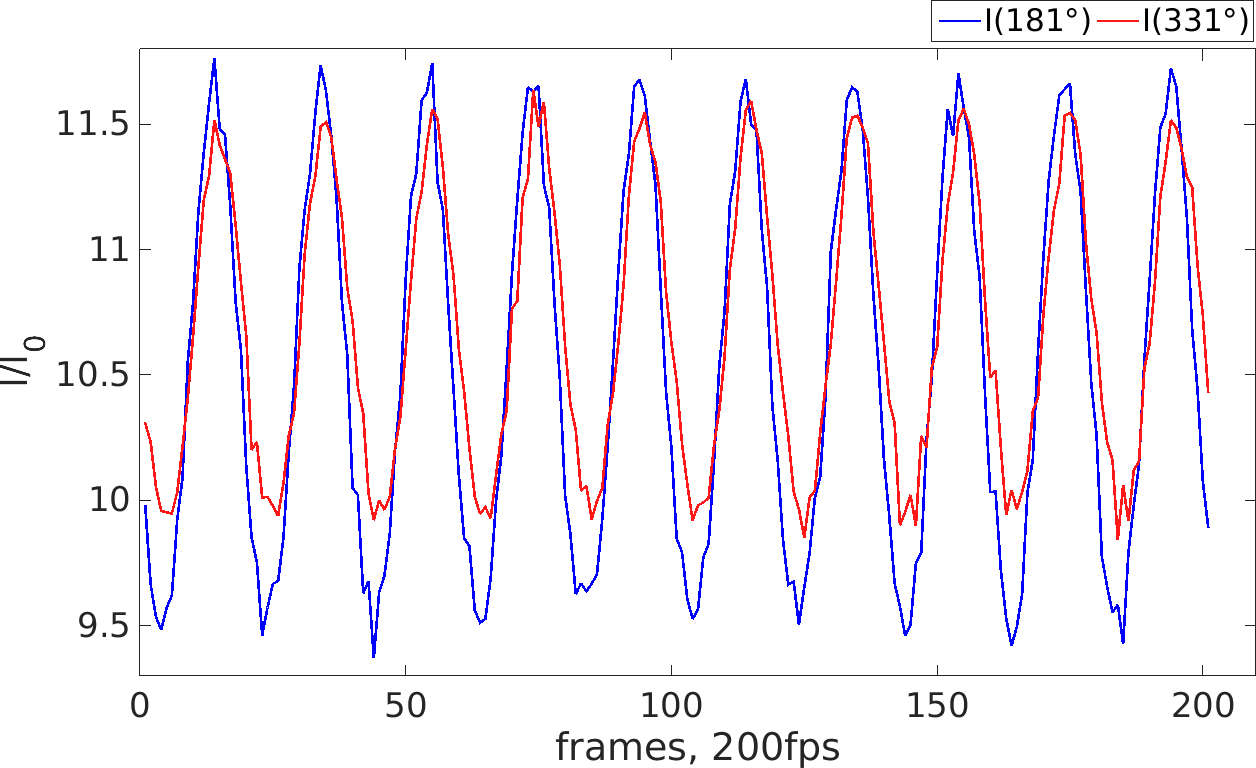
\includegraphics[width=0.7\textwidth,height=0.4\textwidth]{figs/auswertung/plasmaglw/intensdipol181u3313Hz1sek.png}
						\caption{Vergleich der Intensitätsverläufe bei $\unit[149]{\degree}$  und $\unit[331]{\degree}$ der Dipol-Anregung von \ref{img:randfrequenz} bei $\unit[3]{Hz}$ für $\unit[1]{s}$. $I\left(\varphi=\unit[331]{\degree}\right)$ ist um 33 \tilt{frames} verzögert, damit die Extrema übereinander liegen.}
						\label{img:intensdipol}
					\end{figure}

				Mit den Ergebnissen der \ref{img:randfrequenz} bis \ref{img:randhochutiefrotat} ist die Methodik der Versuche um das Plasma-Glow prinzipiell bestätigt. Die Potentiale auf der Ring-Elektrode beeinflussen die Randschicht in dessen näherer Umgebung. Das kann man der lokalen Veränderung des Leuchtens in Folge der Manipulation entnehmen. Diese Einflüsse sind nur auf Zeitskalen der Cluster-Dynamik (Sekunden, Herz) und den räumlichen Dimensionen des Ringes (Zentimeter) von Bedeutung. Das Verhalten der Rand- bzw. Vorschicht während der \tilt{rf}-Zyklen spielte keine Rolle in den vorher gemachten Beobachtungen. Es kann demnach gefolgert werden, dass durch die Anregung mit der segmentierten Elektrode das lokale Potential verändert wird. Insbesondere kann daraus geschlossen werden, dass die Manipulation eines Yukawa-Clusters eindeutig durch die elektrostatische Wechselwirkung direkt mit dem Ring und dem abgewandelten Einfang erfolgt. Auf Grundlagen dessen sollen nun konkrete Analysen und Interpretationen vorgenommen werden.

				\paragraph{Dipol-Anregung}

						\begin{figure}[!t]
							\centering
							\begin{subfigure}{0.49\textwidth}
								\centering
								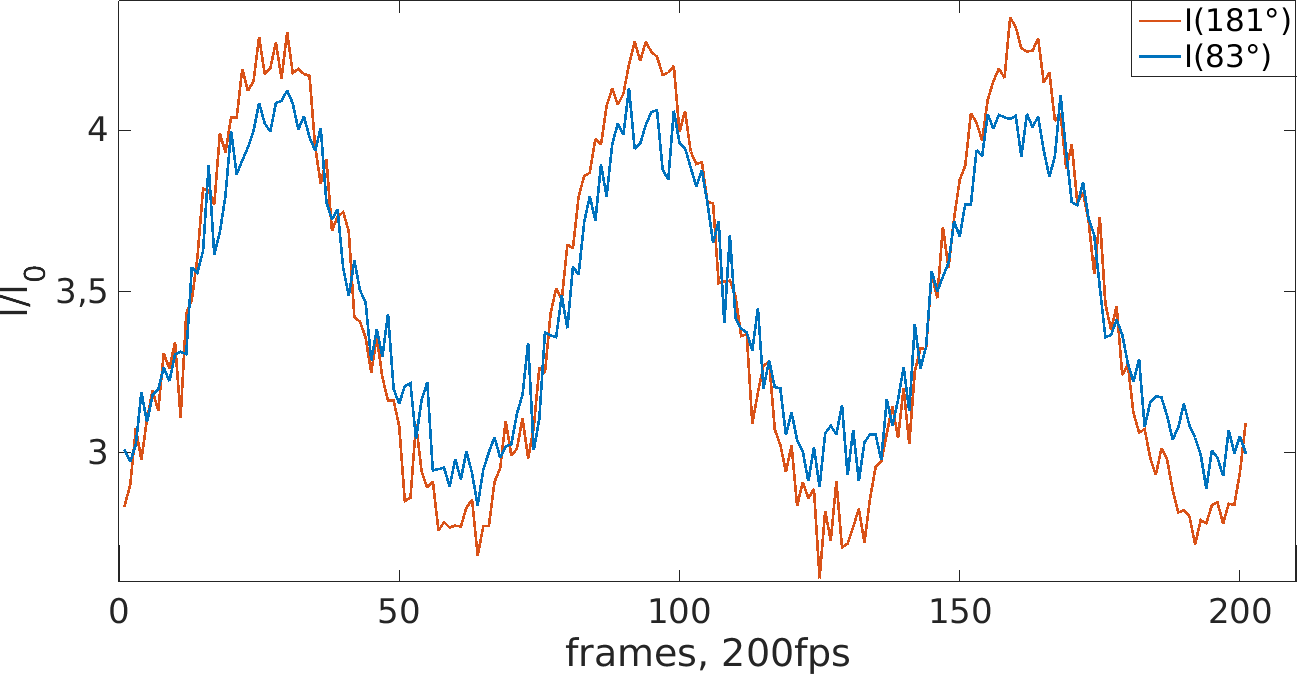
\includegraphics[width=\textwidth,height=0.65\textwidth]{figs/auswertung/plasmaglw/intens83u180quadinphase3Hz1sek.png}
							\end{subfigure}
							\begin{subfigure}{0.49\textwidth}
								\centering
								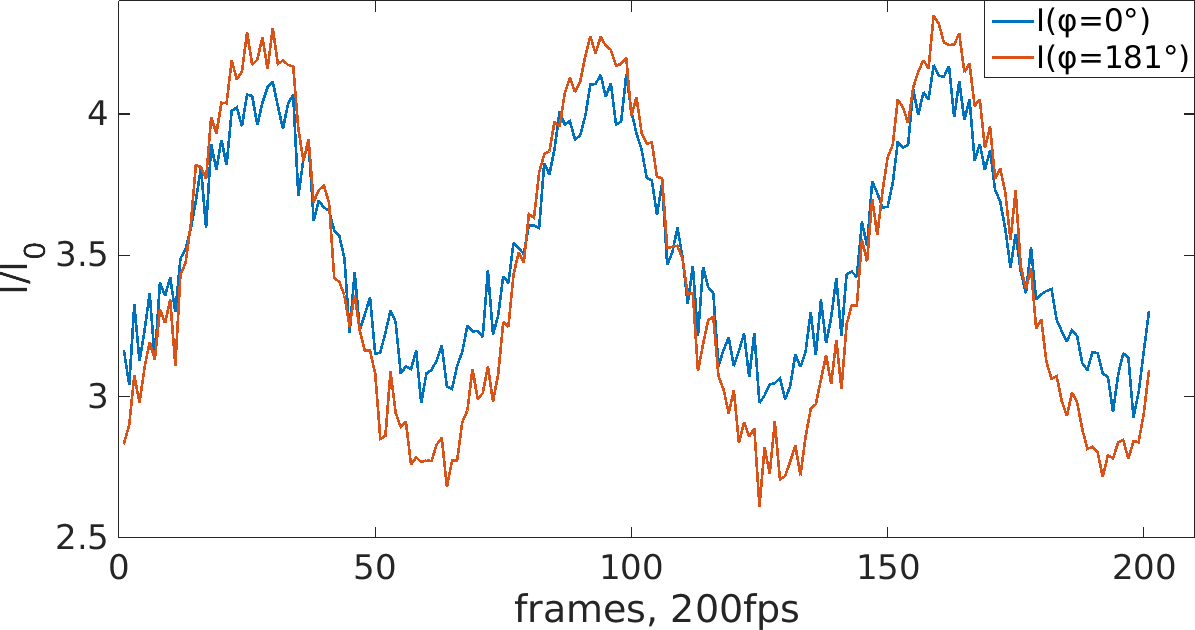
\includegraphics[width=\textwidth,height=0.65\textwidth]{figs/auswertung/plasmaglw/intens0u180quad3Hz1sek.png}
							\end{subfigure}
							\caption{Intensitätsverläufe der Quadrupol-Anregung aus \ref{img:randhochutiefwink}:\underline{\fett{links}} bei $\unit[3]{Hz}$ für $\unit[1]{s}$. \underline{\fett{links}:} Bei $\unit[181]{\degree}$ und $\unit[83]{\degree}$. $I\left(83\degree\right)$ ist um 33 \tilt{frames} verzögert. \underline{\fett{rechts}:} Für $\unit[181]{\degree}$  und $\unit[0]{\degree}$. }
							\label{img:intensquadhochwink}
						\end{figure}

					Die für \ref{img:randfrequenz} besprochenen Unterschiede zwischen den Extrema der beiden Pole lassen sich leicht in einem direkten Vergleich ablesen. Dabei werden die zeitlichen Verläufe der Helligkeit der Winkel $\unit[149]{\degree}$, genannt $\Phi$, und $\unit[331]{\degree}$, als $\Theta$ bezeichnet, mit ihren Maxima und Minima übereinander gelegt, damit direkt die Differenzen eingesehen werden können. In \ref{img:intensdipol} ist , für das gleiche Zeitintervall wie es in \ref{img:randfrequenz} dargestellt wurde, dieser Vergleich vorgenommen worden. Man erkennt leicht die Unterschiede zwischen den Amplituden der Intensität: sowohl maximale als auch minimale Helligkeit in Richtung von $\Phi$ sind stärker ausgebildet als die von $\Theta$. Diese Differenz beträgt im Mittel 3\%. Jedoch sind die Unterschiede zwischen den Minima größer als die der Maxima.\\
					Vergleicht man die Winkelanordnung der zwei benannten Pole mit der Maske aus \ref{img:randmaske}, so sieht man, dass diese, ebenso wie bei einem "`echten"' Dipol, 2 gegenüberliegenden Segmenten des Ringes entsprechen. Diese Feststellung ist in Einklang mit den Erwartungen an diese Untersuchung. Hingegen weniger diesen entsprechend, ist die Differenz zwischen den Extrema der Intensität, welche zu jeweils 2 zusammen gelegten Segmenten gehörten. Wie bereits erwähnt, manipuliert der Pol $\Phi$ den Glow in seiner Umgebung stärker als $\Theta$. In der Richtung von $\Phi$ findet sich außerdem der Arm der Ring-Elektrode. Dessen Randschicht ragt in den Ring hinein und geht in die anliegenden Segmente über. Die Vermutung ist nun, dass sich deswegen die Randschichten der umliegenden Segmente und deren Glow verändert. Auf diese Weise kann besonders gut die stärkere Ausprägung der Minima von $\Phi$ erklärt werden. Andererseits beschreibt diese theorie nicht, warum ebenso in den Maxima ein signifikanter Unterschied besteht. Eine Möglichkeit das zu erklären ist, dass die Isolierung der Befestigung nicht lückenlos bzw. der Ring nicht vollkommen symmetrisch war. Demnach handelt es sich bei dieser Inhomogenität um einen systematischen Fehler.

						\begin{figure}[!b]
							\centering
							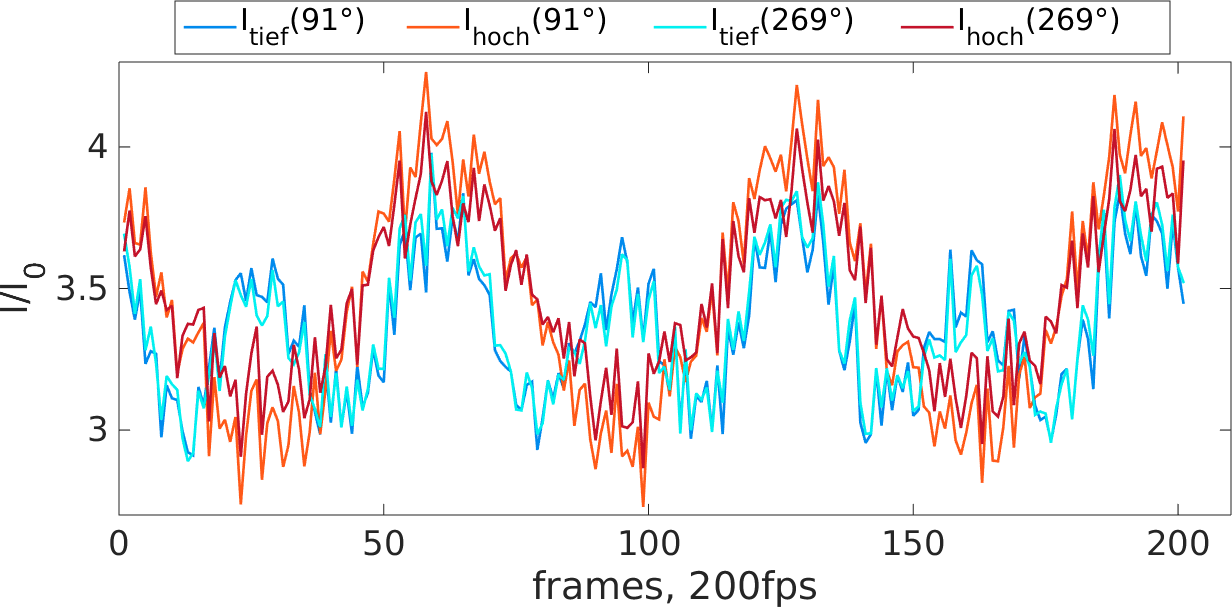
\includegraphics[width=0.8\textwidth,height=0.45\textwidth]{figs/auswertung/plasmaglw/intens270u90hochutiefquad3Hz1sek.png}
							\caption{Intensitätsverläufe bei $\unit[91]{\degree}$ und $\unit[269]{\degree}$ der Quadrupol-Anregung aus \ref{img:randhochutiefwink} für einen hohen und tiefen Ring, bei $\unit[3]{Hz}$ für $\unit[1]{s}$. }
							\label{img:intensquadhochutief}
						\end{figure}

				\paragraph{Quadrupol-Anregung}

					Für den Verlauf der Helligkeit aus \ref{img:randhochutiefwink}:\underline{\fett{links}} \ref{img:intensquadhochwink} die, analog zur Analyse der Dipol-Schwingung, entsprechende Grafik. Für die beiden Vergleiche - einerseits zwischen den Achsen $\Sigma$ und $\Pi$ in \ref{img:intensquadhochwink}:\underline{\fett{links}}, als auch für eine Achse $\Pi$ in \ref{img:intensquadhochwink}:\underline{\fett{rechts}} - zeigen sich ähnliche Verhältnisse wie im vorherigen Abschnitt. In Richtung des Elektroden-Armes um $\varphi\approx\unit[150]{\degree}$ findet man allgemein stärkere Extrema vor. Konkret liegen die Intensitäten 3\%-5\% auseinander. Was jedoch die Vermutung der Beeinflussung der Randschicht durch den Ausleger bestätigt, ist der Unterschied zwischen den Differenzen in den beiden Bildern: für $I(\varphi=\unit[83]{\degree})$ finden sich näherungsweise gleiche Minima wie für $I(\varphi=\unit[181]{\degree})$. Dies ist jedoch nicht der Fall bei $I(\unit[0]{\degree})$. Des Weiteren kann auch die Vermutung über die Inhomogenität bekräftigt werden. Da bei der Quadrupol-Anregung jedes Segment um jeweils $\unit[90]{\degree}$ in der Phase verschoben war, sind die Extrema diesen eindeutig zuzuordnen. Daher kann aus den Unterschieden der vergleichenden Graphen auf die Asymmetrie des Ringes bzw. Fehler in der Fertigung dessen geschlossen werden.

						\begin{figure}[!t]
							\centering
							\begin{subfigure}{0.49\textwidth}
								\centering
								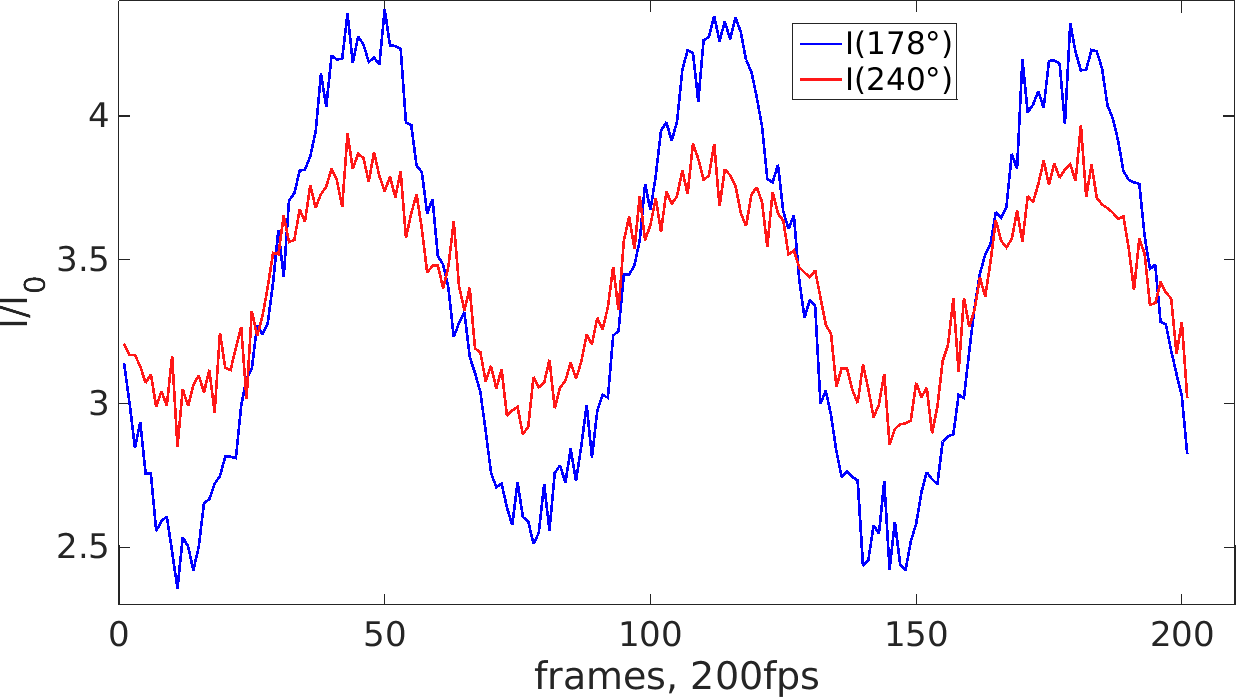
\includegraphics[width=\textwidth,height=0.65\textwidth]{figs/auswertung/plasmaglw/intensrotathoch178u2402Hz1sek.png}
							\end{subfigure}
							\begin{subfigure}{0.49\textwidth}
								\centering
								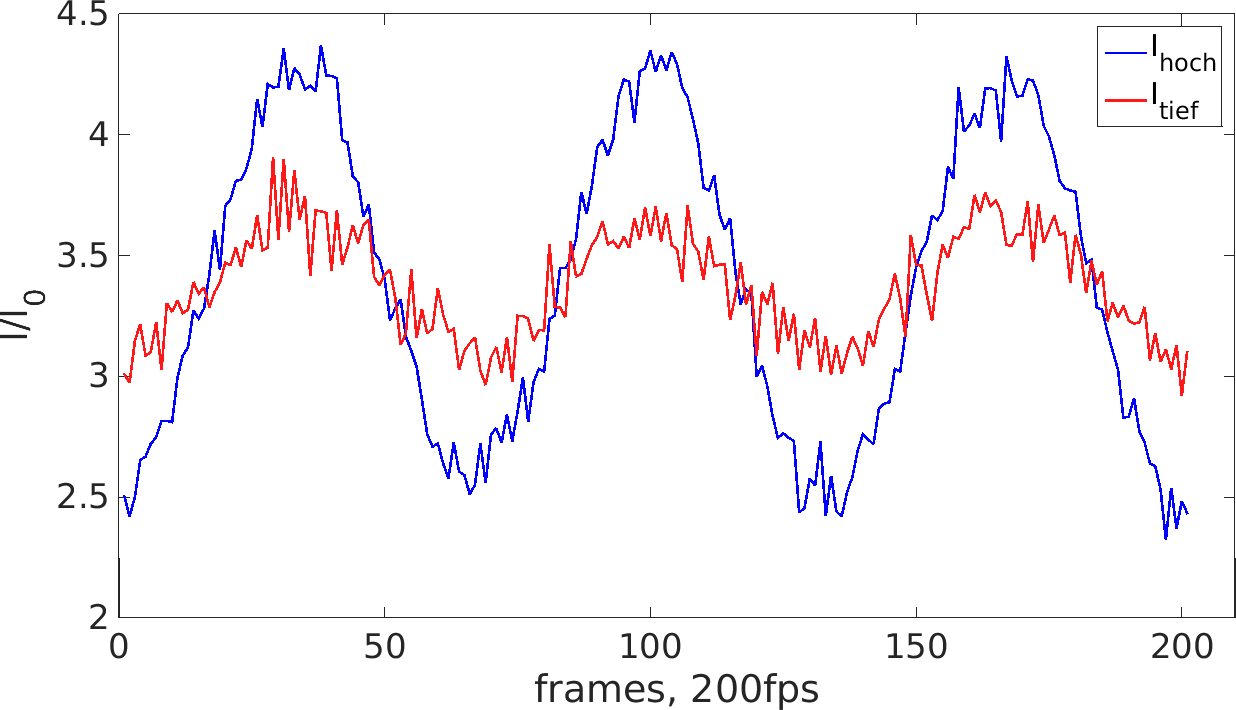
\includegraphics[width=\textwidth,height=0.65\textwidth]{figs/auswertung/plasmaglw/intensrotathochutief1783Hz1sek.png}
							\end{subfigure}
							\caption{Intensitätsverläufe einer Rotations-Anregung bei $\unit[3]{Hz}$ für $\unit[1]{s}$. \underline{\fett{links}:} Vergleich zweier Richtungen bei hoher Ring-Elektrode. $I\left(178\degree\right)$ ist um 33 \tilt{frames} verzögert. \underline{\fett{rechts}:} Für einen Winkel für unterschiedliche Höhen.}\label{img:intensrotathochutief}
						\end{figure}

						\begin{figure}[!b]
							\centering
							\begin{subfigure}{0.49\textwidth}
								\centering
								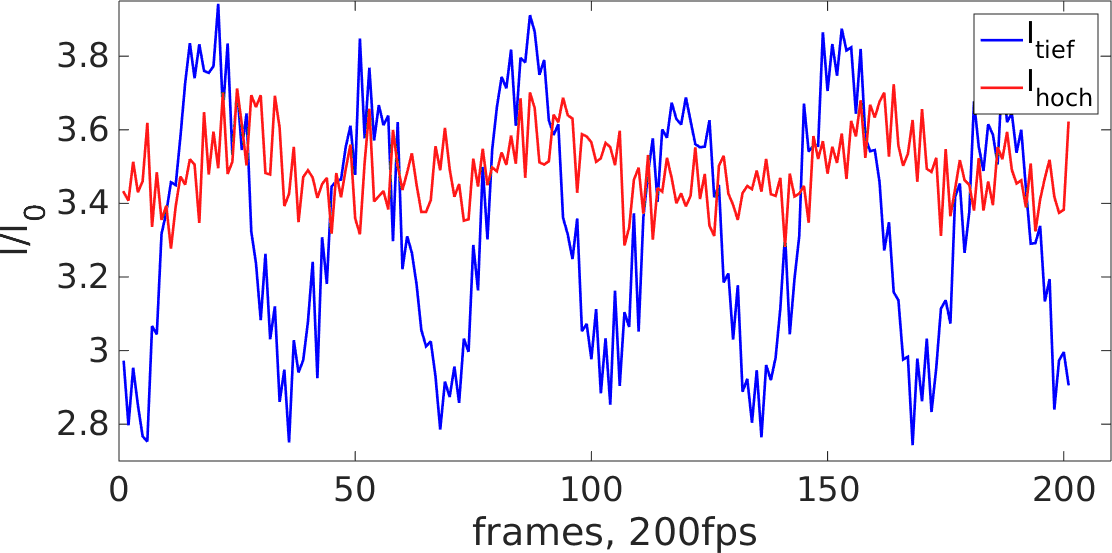
\includegraphics[width=\textwidth,height=0.65\textwidth]{figs/auswertung/plasmaglw/intenshochutiefquadin3Hz1sek.png}
							\end{subfigure}
							\begin{subfigure}{0.49\textwidth}
								\centering
								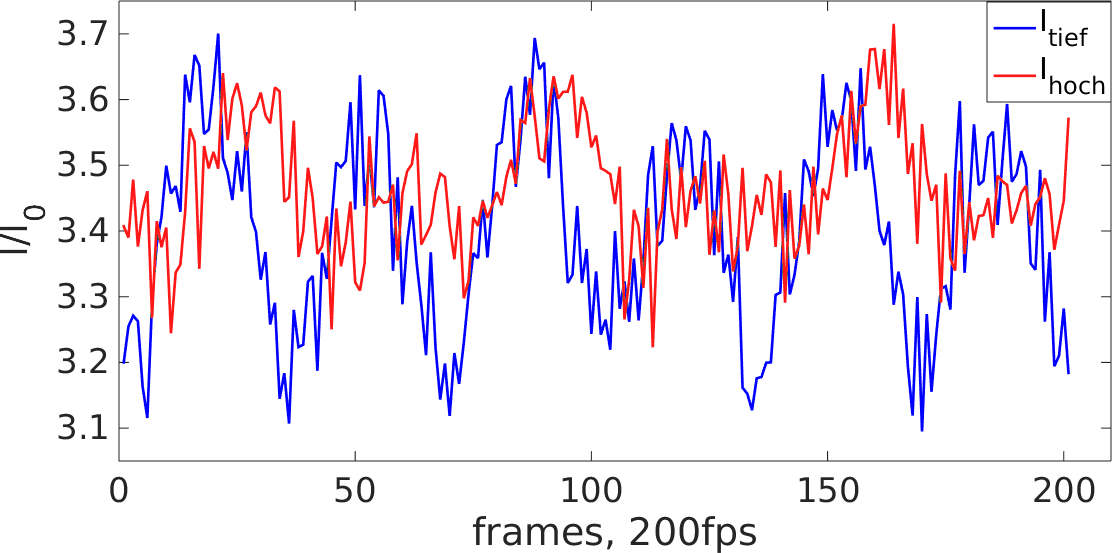
\includegraphics[width=\textwidth,height=0.65\textwidth]{figs/auswertung/plasmaglw/intenshochutiefquadout3Hz1sek.png}
							\end{subfigure}
							\caption{Intensitätsverläufe bei radialer Auflösung für eine Quadrupol-Anregung bei $\unit[3]{Hz}$ für $\unit[1]{s}$. \underline{\fett{links}:} Vergleich hoher und tiefer Elektrode bei $R=0$. \underline{\fett{rechts}:} Für $R=R\ix{max}$.}\label{img:intensquadhochutiefrad}
						\end{figure}

					Mit \ref{img:intensquadhochutief} schließt sich der Vergleich zweier ausgewählter Richtungen (Segment 4 und 2) für unterschiedliche Ring-Höhen an. Deutlich erkennt man die insgesamt niedrigere Intensität für einen tiefen Ring. Auch ist die verschwindend geringe Differenz zwischen den Intensitäten der gegenüberliegenden Segmente auffällig. Das ist in Einklang mit den vorherigen Ausführen. Eine Überraschung stellt jedoch das zusätzliche Maximum dar, welches an Stelle der Minima der Graphen für eine hohe Elektrode auftaucht. Dieses wurde bereits in \ref{img:randhochutiefwink}:\underline{\fett{rechts}} beobachtet und kann somit hier bestätigt werden. Hängt der Ring nahe genug über der Elektrode (einer Metalloberfläche), so kann eine Oszillation des Glows mit der doppelten Frequenz der Anregung in der Mitte des Ringes beobachtet werden. Bei der Quadrupol-Anregung liegen dementsprechend, während einer Periode zwei mal, gleichzeitig Maxima und Minima auf den Segmenten der beiden Schwingungsachsen. Darauf baut die Vermutung auf, dass die Randschicht-Verformung dieser Potentiale groß genug ist, damit auch die Ring-Mitte dunkel wird. Das manifestiert sich als Minimum (in \ref{img:randhochutiefwink}:\underline{\fett{rechts}}) vor und nach dem neuen Maximum (\ref{img:intensquadhochutief}). Liegen wiederum nur schwache oder keine Potentiale auf den Segmenten, so kehrt das Plasma innerhalb des Ringes in den Ausgangszustand zurück und es kann wieder das Leuchten beobachtet werden. Die Schwingung des Plasma-Glow in der Mitte hat gerade die doppelte Frequenz der Anregung. Diese Beobachtung bzw. Entdeckung wird im weiteren Verlauf der Auswertung eine wichtige Rolle spielen, da sie mit dieser Art der Manipulation nicht beabsichtigt war.\\
					Die \ref{img:intensquadhochutiefrad} zeigt Vergleiche der Intensitätsverläufe bei hoher und niedriger Elektrode für die Mitte $R=0$ und den Rand des Ringes $R=R\ix{max}$. Die Daten der Graphen entsprechen denen der Darstellung aus \ref{img:randhochutiefrad} sowie \ref{img:randhochutiefwink}. In den beiden Grafiken sind nochmals, gut deutlich, die Kontraste zwischen den sehr scharfen Extrema einer niedrig angebrachten Anregung und der verschmierten Verteilung der Helligkeit eines hohen Ringes zu sehen. Insbesondere können damit die vorher nur zu erahnenden Maxima bestätigt werden, sind sie dennoch verschwindend klein. Wiederum ist die Intensität bei einer niedrigen Höhe für die entsprechenden Minima wesentlich geringer. Es finden sich zudem 6 Extrema bei einer Anregung von $\unit[3]{Hz}$: das Leuchten innerhalb des Ringes schwingt mit. Beim maximalen Radius sind hingegen die Extrema von $I\ix{tief}$ weniger und die von $I\ix{hoch}$ stärker ausgeprägt. Das ist Folge der Nähe zur Quelle der Anregung. Durch das Mitteln über ein Radius-Intervall und einen vollen Winkelbereich, gehen in die Intensität des letzten Abschnitts sowohl dunkle Randschichten als auch helles Glow mit ein. Direkt an den Segmenten geschehen demnach signifikante Veränderungen der Grenzschicht des Plasmas, was mit dem Konzept des Ringes in Einklang ist.

				\paragraph{Rotations-Anregung}

					Abschließend erfolgt eine Betrachtung der Intensitäten bei einer Rotations-Anregung. Hierbei werden einerseits in \ref{img:intensrotathochutief}:\underline{\fett{links}} die, für \ref{img:randhochutiefrotat} besprochenen, charakteristischen Winkel bei denen Inhomogenitäten auftraten, verglichen. Andererseits zeigt \ref{img:intensrotathochutief}:\underline{\fett{rechts}} den Verlauf der Helligkeit des selben Winkelelements bei verschiedenen Ring-Höhen. Die erste Grafik gibt deutlich die Asymmetrien der Segmente 1 und 3 wieder, wie sie zuvor mehrmals beobachtet wurden. Die Differenz in der Intensität liegt im Mittel zwischen 7\% und 8\%. Der zweite Vergleich zeigt die schwachen Extrema einer Rotation bei einem kleinen Abstand zur Randschicht der Elektrode. Da bei dieser Anregung jeweils nur eines der Segmente ein minimales Potential tr\"agt, w\"ahrend die anderen schwach negative bzw. maximale haben, ist der Intensitätsverlauf innerhalb des Ringes nicht-trivial. Im Bereich um das Element mit dem kleinsten Potential ist der Glow, auf Grund der in diesem Augenblick Massepotential tragenden angrenzenden Segmente, stark verändert. Das \"ubrige Segment hat zu dieser Zeit ein Maximum und zeigt das, zum Minimum umgekehrte Verhalten. Insgesamt ist das, auf einer Ring-Bahn ``wandernde'' Leuchten (bzw. Dunkel) wesentlich kontrast\"armer. Die \tilt{hot-spots} aus \ref{img:randhochutiefrotat} k\"onnen, mit der gewonnenen Kenntnis, in etwa als die Mittelpunkte der Segmente identifiziert werden, was nahe legt, dass dort die Glow-Manipulation am st\"arksten ist. Jedoch spricht dies nicht f\"ur die Qualit\"at des Ringes als symmetrische Multipol-Elektrode. Insbesondere findet kann stetiger Übergang zwischen den Segmenten statt, da dort ein etwa $\unit[1]{mm}$ breiter Bereich ohne Kupfer frei liegt.

						\begin{figure}[!t]
							\centering
							\begin{subfigure}{0.49\textwidth}
								\centering
								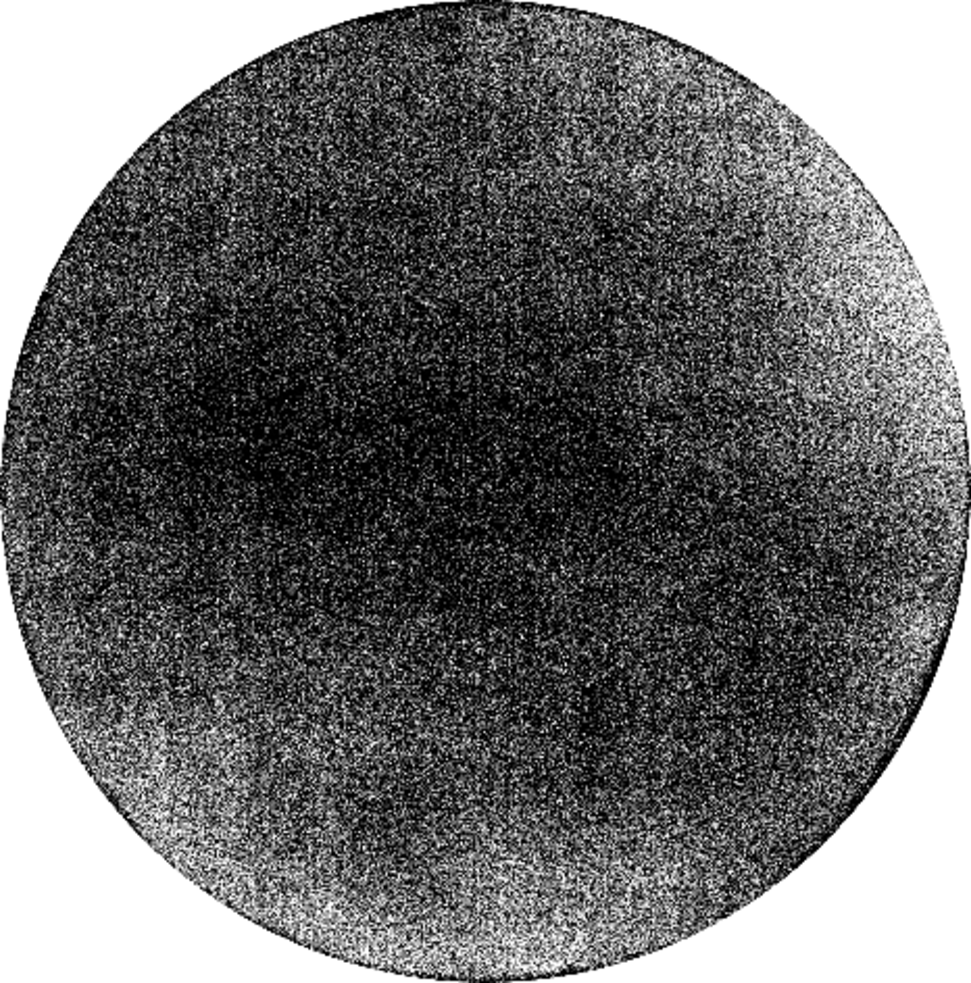
\includegraphics[width=0.5\textwidth,height=0.5\textwidth]{figs/auswertung/plasmaglw/beispieldipolglownu.pdf}
							\end{subfigure}
							\begin{subfigure}{0.49\textwidth}
								\centering
								\includegraphics[width=0.5\textwidth,height=0.5\textwidth]{figs/auswertung/plasmaglw/beispieldipolglow.pdf}
							\end{subfigure}
							\caption{Ausschnitt aus zwei Bildern der oberen Kamera 'grün' bei einer Dipol-Anregung. Links erliegt die Manipulation. Rechts tragen zwei der vier Segmente, welche zusammengelegt wurden, ein Extremum.}
						\end{figure}

				\subsubsection*{Fazit}

						Die Analyse des Plasma-Glow in der näheren Umgebung der Manipulations-Elektrode hat Aufschlüsse über die Veränderungen in der Randschicht ergeben. Insbesondere für eine niedrigere Höhe, in welcher später der Yukawa-Ball eingefangen wird, konnten interessante Beobachtungen gemacht werden. Insgesamt hat die Untersuchung einen Einblick dahin gehend ermöglicht, welche Effekte der Anregung und dem Einfang des Clusters zu Grunde liegen. Des Weiteren konnten bereits mögliche Fehlerquellen späterer Messungen erfasst werden.

			\newpage

		\subsection{Elektrische Manipulation}

			In diesem Abschnitt werden die Messergebnisse der Beobachtungen der unterschiedlichen Manipulationen eines finiten Yukawa-Clusters präsentiert. Dabei wird zuerst auf die Analyse bezüglich der Normalmoden nach Kapitel \ref{subsub:moden} eingegangen. Dem schließt sich entsprechend die Fluidmoden-Betrachtung an. Differenziert wird zusätzlich zwischen den Anregungen mit einer 4- bzw. 6-segmentigen Ring-Elektrode. Die Auswertung der erhaltenen Daten erfolgt mit Rückblick auf die Ergebnisse des vorherigen Abschnitts, da in diesem essentielle Informationen über die Manipulationen mittels der Ring-Elektrode erlangt wurden.

			\subsubsection{Normalmoden-Analyse}

				Die Auswertungen der Normalmoden-Anteile in der Bewegung des Clusters erfolgt über die Betrachtung der spektralen Leistungsdichte $S\ix{p}\left(\omega\right)$. Die daraus ermittelten Eigenmoden, in welchen verstärkt Energie enthalten ist, werden daraufhin einzeln betrachtet und analysiert.\\
				Bei den gemachten Messungen lag der Argon-Gasdruck zwischen $\unit[6,42-10]{Pa}$. Die eingespeisten Leistungen des rf-Generatos lagen, für die Quadrupol-Anregung, bei $\unit[0,5]{W}$ und, in den Versuchen mit der 6-Segment-Elektrode, bei $\unit[1,4]{W}$. Alle drei Kameras nahmen mit einer Auflösung von $\unit[1280]{px}\times\unit[1024]{px}$ bei 100 \tilt{fps} auf. Die Blenden-Öffnungszeit, dass heißt wie lange Licht auf den \tilt{CCD}-Chip treffen kann, betrug $\unit[8]{\upmu s}$. Kamera 'rot' und 'gelb' nahmen jeweils durch $\unit[60]{mm}$, 'gruen' durch ein $\unit[150]{mm}$ Objektiv auf. Jede Messreihe entsprach 10000 Bildern, was bei der gegebenen Frequenz $\unit[100]{s}$ gleich kam.

					\begin{figure}[!h]
						\centering
						\includegraphics[width=\textwidth]{figs/auswertung/manipulation/ersteungestpowerdens.png}
						\caption{Spektrale Energiedichte $S\ix{l}\left(\omega\right)$ für einen ungestörten Cluster von $N=26$ Teilchen. Die besonders angeregten Moden sind mit Pfeilen und den Nummern markiert.}\label{img:powerdensersteungest}
					\end{figure}

	\vspace{-0.4cm}

					\subsubsection*{Ring-Elektrode mit 4 Segmenten}

						Mit diesem Ring sind vier Messungen zur Quadrupol-Anregung bei unterschiedlichen Frequenzen und einer Teilchenzahl von $N=26$ gemacht worden. Jeweils zwei gegenüberliegende Segmente besaßen dabei das gleiche Potential, wobei insgesamt die beiden sinusoidalen Signale mit einer Amplitude von $U\ix{pp}=\unit[10]{V}$ um eine halbe Periode phasenverschoben waren. Speziell angeregte Moden, die anschließend diskutiert werden, sind in den Energiedichten mit Pfeilen hervorgehoben.\\
						Die \ref{img:powerdensersteungest} zeigt die Dichte für einen ungestörten Cluster von $N=26$ bei den oben genannten Parametern. Mit Pfeilen sind die, entweder für einzelne Frequenzen oder über das gesamte dargestellte Spektrum ($\unit[0-50,5]{Hz}$), energiereichsten Moden hervorgehoben. Im Allgemeinen sind für Frequenzen bis $\unit[10]{Hz}$ alle Moden gut angeregt. Deren Energiegehalt ist dabei in Relationen zu den Moden mit dem größten Anteil an der kollektiven Bewegungen des Clusters dargestellt. Diese Verteilung ist Folge des "`thermischen Chaos"': die zufälligen \tilt{brownschen} Bewegungen der levitierenden Staubpartikel, welche mit bloßem Auge als Zittern wahrnehmbar waren, enthalten viele Moden gleicher Maßen. Die Eigenmoden bzw. -vektoren, welche der Cluster nach Gl.(\ref{eq:ewp}) enthält, sind orthogonal zueinander. Die  thermischen Geschwindigkeitsvektoren $v\ix{th}\left(t\right)$ erfüllen diese Eigenschaft insbesondere nicht, weswegen diese für die Konstruktion der Kollektivbewegung aus vielen verschiedenen Moden zusammengesetzt werden müssen. Speziell die Moden mit der Nummer 35 und höher enthalten mehr Energie. Sie entsprechen chaotischen, voneinander unabhängigen Ein-Teilchen-Translationen.

					\begin{figure}[!t]
						\centering
						\begin{subfigure}[t]{0.325\textwidth}
							\centering
							\includegraphics[width=\textwidth,height=0.8\textwidth]{figs/auswertung/manipulation/erstensungestModeNr42.png}
						\end{subfigure}
						\begin{subfigure}[t]{0.325\textwidth}
							\centering
							\includegraphics[width=\textwidth,height=0.8\textwidth]{figs/auswertung/manipulation/erstensungestModeNr19.png}
						\end{subfigure}
						\begin{subfigure}[t]{0.325\textwidth}
							\centering
							\includegraphics[width=\textwidth,height=0.8\textwidth]{figs/auswertung/manipulation/erstensungestModeNr43.png}
						\end{subfigure}
						\begin{subfigure}[t]{0.325\textwidth}
							\centering
							\includegraphics[width=\textwidth,height=0.8\textwidth]{figs/auswertung/manipulation/erstensungestModeNr9.png}
						\end{subfigure}
						\begin{subfigure}[t]{0.325\textwidth}
							\centering
							\includegraphics[width=\textwidth,height=0.8\textwidth]{figs/auswertung/manipulation/erstensungestModeNr23.png}
						\end{subfigure}
						\caption{Die Eigenvektoren (blau) der Moden mit den entsprechenden Nummern. In schwarz sind die zu erkennenden Kollektivbewegungen eingezeichnet. Die Auswahl bezieht sich auf die Betrachtungen zu \ref{img:powerdensersteungest}. Die erste Reihe zeigt die Moden 19, 42, 43. Reihe zwei enthält Nummer 9 und 23.}\label{img:modenersteungest}
					\end{figure}

				Interessant sind die markierten Nummern (siehe \ref{img:modenersteungest}), welche, u.a. über den genannten Bereich hinaus, größere Werte der spektralen Dichte haben. Die Moden 8 und 9 entsprechen Cluster-Rotationen mit einer, zur xy-Ebene parallelen  Drehachse. Sie sind zueinander konjugiert, dh. links- und rechts-drehend (damit orthogonal). Deren korrespondierender Eigenwert liegt, in Übereinstimmung mit Abschnitt \ref{subsub:moden}, bei verschwindend kleinen Frequenzen bzw. bei $\unit[0]{Hz}$. Die Moden 19, 42 und 43 bilden ein, im Sinne eines kartesischen Koordinatensystems, rechtwinkliges Tripel der Clusterbewegung. Jeweils eine dieser Lösungen des Eigenwertproblems zeigt in Richtung einer Achse des Raumes. Des Weiteren stellt Nummer 23 eine Rotation um eine, zur z-Richtung parallelen Achse dar. Die Moden 56, 61 und 65 sind chaotische Bewegungen: die Eigenvektoren haben keine "`besondere"' Anordnung.\\
				Die rechtwinkligen Moden 19, 42 und 43 spiegeln die chaotisch-thermischen Bewegungen der Partikel wieder: aus ihnen kann jede beliebe Bewegung konstruiert werden. Die Nummern 8, 9 und 23 kommen durch die Anordnung der Laserstrahlen zustande: die Strahlen sind nicht exakt auf den Mittelpunkt des Clusters fokussiert. Da über deren Querschnitt ein Photonendichte-Gradient existiert, erfahren einige Teile des Yukawa-Balls andere Kräfte durch den unterschiedlichen Strahlungsdruck. Daraus resultiert eine Rotation vom Strahlungsmaximum weg. Da zwei Laser auf den Cluster gerichtet sind, ist es u.U. möglich, dass er um mehrere Achsen rotiert oder seine Gesamtrotation aus verschiedenen zusammengesetzt ist. Daher finden sich mehrere angeregte, dafür zuständige Moden im Spektrum. Für tiefgreifendere Ausführungen zu Laser-induzierten Rotationen siehe \cite{Mulsow13}. Der Kontrast zwischen den Energien niedriger Frequenzen bis $\unit[10]{Hz}$ und darüber resultiert aus den Eigenschaften der \tilt{brownschen} Bewegung.

					\paragraph{Quadrupol-Schwingungen bei 1\,Hz}

							\begin{figure}[!b]
								\centering
								\includegraphics[width=\textwidth]{figs/auswertung/manipulation/quadrupol1Hzpowerdens.png}
								\caption{Spektrale Energiedichte für einen Cluster von $N=26$ Teilchen bei einer Quadrupol-Anregung mit $\unit[1]{Hz}$. Es sind angeregte, höhere Harmonische der Schwingung bei $\unit[2]{Hz}$ zu sehen.}\label{img:powerdensquadrupol1Hz}
							\end{figure}

						In \ref{img:powerdensquadrupol1Hz} ist die Energiedichte zu sehen. Die Nummern 17, 45 und 46 entsprechen hier den rechtwinkligen Kollektionen der Eigenvektoren wie in \ref{img:modenersteungest}. In diesem Fall enthalten sie im Vergleich zum übrigen Spektrum mehr Energie. Das ist offensichtlich Resultat der Anregung: die Quadrupol-Mode besteht aus Translationen bzw. Cluster-Deformationen auf den Schwigungsachsen. Im speziellen enthält die Nummer 17 eine vergleichbare Energie wie ihre Partner. Jedoch kommt in einer zweidimensionalen Quadrupol-Anregung natürlich keine vertikale Komponente vor. Die Schwingung in z-Richtung ist demnach Folge der Randschichtveränderung in der Mitte des Ringes durch dessen elektrostatische Wechselwirkung mit dem Plasma. Als Referenz sei der vorherige Abschnitt \ref{sub:glowanalys} der Analyse des Plasma-Glow angegeben. Diese vertikale Oszillation enthält besonders viel Energie bei $\unit[2]{Hz}$, da das "`durchschwingen"' der Randschicht gerade mit dem Zweifachen von $\omega$ geschieht.\\
						Sehr scharfe Maxima der Dichte sind bei $\unit[1]{Hz}$ zu sehen. Das zweite, bei einem natürlichen (zwei) Vielfachen der Frequenz auftauchende Maximum entspricht einer höheren Harmonischen der Schwingung. Diese sind gut bei den Moden 24, 26, 29, 45 und 46 zu erkennen. Die Nummern 6, 24 und 29 sind entsprechend Rotationsmoden - siehe \ref{img:modenquadrupol1Hz}. Anders ist hierbei jedoch, dass es nicht nur eine Drehachse pro Mode gibt, sondern auch beispielsweise gegenläufige Rotationen in einer zusammenkommen (Nummer 6, 26). Ihre Resonanz liegt hierbei jedoch nicht mehr bei $\unit[0]{Hz}$, sonder ist in etwa um eine Anregungsfrequenz nach oben verschoben. Das legt die Vermutung nahe, dass deren Spektrum sich aus den Bewegungen des Quadrupols zusammensetzt und nicht auf Grund der Laser-Anordnung zustande kommt. Neu ist die \tilt{breathing}-Mode 24: sie entspricht einer Ausdehnung des Yukawa-Balls in der Ebene des Quadrupols (parallele zur xy-Ebene). Diese ist schwächer angeregt, da, während der Schwingung auf einer der beiden Achsen dieser Anregung, der Cluster nur minimal senkrecht dazu gestaucht wird. Die Stauchung hat jedoch, als konjugierte Mode zur Ausdehnung, bei der Projektion auf die Deformation einen großen Anteil an der Bewegung. Die Nummer 11 hat kein scharfes Maximum und enthält nur chaotische Eigenvektor-Anordnungen.

							\begin{figure}[!t]
								\centering
								\begin{subfigure}[t]{0.325\textwidth}
									\centering
									\includegraphics[width=\textwidth,height=0.8\textwidth]{figs/auswertung/manipulation/quadrupol1HzModeNr6.png}
								\end{subfigure}
								\begin{subfigure}[t]{0.325\textwidth}
									\centering
									\includegraphics[width=\textwidth,height=0.8\textwidth]{figs/auswertung/manipulation/quadrupol1HzModeNr24.png}
								\end{subfigure}
								\begin{subfigure}[t]{0.325\textwidth}
									\centering
									\includegraphics[width=\textwidth,height=0.8\textwidth]{figs/auswertung/manipulation/quadrupol1HzModeNr26.png}
								\end{subfigure}
								\caption{Auszug der, für \ref{img:powerdensquadrupol1Hz} betrachteten Moden. Insbesondere stehen hier die neuen Rotationen mit mehreren Drehachsen und die \tilt{breathing}-Mode im Fokus.}\label{img:modenquadrupol1Hz}
							\end{figure}


					\paragraph{Quadrupol-Schwingungen bei 3\,Hz}

							\begin{figure}[!b]
								\centering
								\includegraphics[width=\textwidth]{figs/auswertung/manipulation/quadrupol3Hzpowerdens.png}
								\caption{Spektrale Energiedichte für einen Cluster von $N=26$ Teilchen bei einer Quadrupol-Anregung mit $\unit[3]{Hz}$. Es sind angeregte, höhere Harmonische der Schwingung bei $\unit[6]{Hz}$ zu sehen.}\label{img:powerdensquadrupol3Hz}
							\end{figure}

						In \ref{img:powerdensquadrupol3Hz} sieht man die Energiedichte für eine Quadrupol-Anregung mit $\unit[3]{Hz}$. Neben der Ähnlichkeit zur Energie-Verteilung \ref{img:powerdensquadrupol1Hz} fällt auf, dass der Bereich niedriger Frequenzen (bis $\unit[10]{Hz}$) immer weniger eine Rolle spielt: die Dichte ist dort, in Relationen zu den Maxima bei der Anregungsfrequenz, wesentlich geringer. Das heißt, dass die thermische Bewegung innerhalb des Clusters sehr klein gegen die Auslenkungen durch die Anregung ist.\\
						Insbesondere haben die Moden 17, 44 und 45, welche die rechtwinklige Cluster-Translationen sind, gute Extrema bei der ein- und zweifachen Frequenz. Die Nummer 25 ist eine Rotation um eine, zur z-Richtung parallelen Achse. Die Moden 38 und 72 sind beides einatmende \title{breathing}-Moden, das heißt sie stellen Cluster-Ausdehnungen dar. Die Nummer 73 ist die zur 72 konjugierte: eine ausatmende, zusammenziehende \tilt{breathing}-Mode.\\
						Wie bereits besprochen, erfährt der Cluster während der Schwingung entlang einer Achse des Quadrupols eine Deformation auf der anderen. In dieser Richtung wird er gestaucht und verformt sich somit elliptisch.  Die Moden dieser Bewegung sind 52 und 55, welche weiterhin in \ref{img:modenquadrupol3Hz} gezeigt werden. Diese enthält offensichtlich immer mehr Energie, umso näher die Frequenz an der Eigenfrequenz liegt, weil der Cluster dort die größte Resonanz zeigt. In den Moden der elliptische Deformation ist deswegen signifikant Energie gespeichert: die $\unit[3]{Hz}$ der Anregung liegen in der Nähe von $\omega\ix{0}$. Dies wird ebenso durch den verstärkten Kontrast zu den restlichen Moden bekräftigt. Deren Energiedichte ist, im Vergleich zu den explizit besprochenen sowie der Anregung mit $\unit[1]{Hz}$, viel geringer.

							\begin{figure}[!t]
								\centering
								\begin{subfigure}[t]{0.325\textwidth}
									\centering
									\includegraphics[width=\textwidth,height=0.7\textwidth]{figs/auswertung/manipulation/quadrupol3HzModeNr52.png}
								\end{subfigure}
								\begin{subfigure}[t]{0.325\textwidth}
									\centering
									\includegraphics[width=\textwidth,height=0.7\textwidth]{figs/auswertung/manipulation/quadrupol3HzModeNr55.png}
								\end{subfigure}
								\begin{subfigure}[t]{0.325\textwidth}
									\centering
									\includegraphics[width=\textwidth,height=0.7\textwidth]{figs/auswertung/manipulation/quadrupol3HzModeNr73.png}
								\end{subfigure}
								\caption{Auswahl der angeregte Moden einer Quadrupol-Schwingung bei $\unit[3]{Hz}$. Neu sind Moden 52 un 55 als elliptische Deformationen während der Auslenkung auf einer Achse.}\label{img:modenquadrupol3Hz}
							\end{figure}

							\begin{figure}[!h]
								\centering
								\includegraphics[width=\textwidth]{figs/auswertung/manipulation/quadrupol5Hzpowerdens.png}
								\caption{Spektrale Energiedichte für einen Cluster von $N=26$ Teilchen bei einer Quadrupol-Anregung mit $\unit[5]{Hz}$. Es sind angeregte, höhere Harmonische der Schwingung bei $\unit[10]{Hz}$  und $\unit[15]{Hz}$ zu sehen.}\label{img:powerdensquadrupol5Hz}
							\end{figure}

				\newpage

					\paragraph{Quadrupol-Schwingungen mit 5\,Hz}

						Die \ref{img:powerdensquadrupol5Hz} liefert keine zusätzlichen Informationen über neue, angeregte Moden. Die Nummern 7, 12, 33, 37, 39, 62 und 66 sind chaotisch angeordnete Eigenvektor-Kollektionen. Sie tragen auch hier wiederum signifikant Energie, weil auch aus ihnen alle Cluster-Bewegungen anteilig zusammengesetzt werden können. Analog dazu sind mit 18, 44 und 45 die rechtwinkligen Moden eingetragen. Sie enthalten, der Anregung entsprechend, die meiste Energie. Die Nummern 5, 6 und 32 stellen im Spektrum die Rotationsbewegungen dar.  Hinzu kommen mit 53, 56 und 58 die Quadrupol-Deformationen nach Vorbild von \ref{img:modenquadrupol3Hz}. Die Nummer 31, 70 und 75 enthalten schließlich ein- bzw. ausatmende (relaxierend, kontrahierend) \tilt{breathing}-Moden.\\
						Die 42 entspricht einer, aus der rechtwinkligen Mode und dessen Konjugiertem zusammengesetzte Bewegung. Der Cluster schwingt dabei entlang einer Achse auf seinen Schwer- bzw. Mittelpunkt zu. Das liefert jedoch keine neuen Informationen über die Kinematik des Systems, da diese Bewegung bereits durch die kollektive Translation in einer Richtung (Nummer 44, 45 und siehe die Moden 42, 43 aus \ref{img:modenersteungest}) ausgedrückt wird. Sowohl die Resonanz bei der Anregungsfrequenz, als auch der nächsten (bzw. für die Mode 44 übernächsten) Harmonischen sind gut im Spektrum zu sehen.\\
						Insgesamt hat die Dichte im niederfrequenten Bereich, im Vergleich zu \ref{img:powerdensquadrupol3Hz}, zugenommen, woraus sich schließen lässt, dass der Schritt zu $\unit[5]{Hz}$ die Entfernung zur Resonanzfrequenz $\omega\ix{0}$ vergrößert hat. Ebenso ist auch mehr Energie, als bei einer Anregung von $\unit[3]{Hz}$, in den "`chaotischen"' Moden gespeichert. Das ist als direkte Folge der größeren Differenz zur Eigenfrequenz des Clusters zu verzeichnen. 

				\subsubsection*{Ring-Elektrode mit 6 Segmenten}

%						\begin{figure}[!b]
%							\centering
%							\includegraphics[width=\textwidth]{figs/auswertung/manipulation/zweiteungestpowerdens.png}
%							\caption{Spektrale Energiedichte für einen ungestörten Cluster von $N=31$ Teilchen.}\label{img:powerdenszweiteungest}
%						\end{figure}

					Die Versuche mit der Ring-Elektrode mit 6 Segmenten umfasste Anregungen einer Dipol- und rotieren Dipol-Schwingung. Für den ersten Fall wurden jeweils die Segmente einer Ringhälfte zusammengelegt, sowie mit einer Phasenverschiebung von $\unit[180]{\degree}$ zueinander und Amplitude von $\unit[10]{V}$ \tilt{peak-to-peak} bei verschiedenen Frequenzen versehen. Für die Realisierung eines rotierenden Dipols trugen jeweils 2 gegenüberliegende Segmente das gleiche, sinusoidale Signal. Aufeinander folgende Segmentpaare hatten zueinander eine Phasendifferenz von $\unit[120]{\degree}$, woraus eine Rotationsgeschwindigkeit von einem Ringumfang pro Periode resultierte.

						\begin{figure}[!b]
							\centering
							\includegraphics[width=\textwidth,height=0.5\textwidth]{figs/auswertung/manipulation/dipol1Hzpowerdens.png}
							\caption{Spektrale Energiedichte für eine Dipol-Anregung  bei $\unit[1]{Hz}$ eines Cluster von $N=31$ Teilchen.}\label{img:powerdensdipol1Hz}
						\end{figure}

%					Die \ref{img:powerdenszweiteungest} zeigt die spektrale Energiedichte für einen ungestörten Cluster im 6-Segment-Ring. Analog zu \ref{img:powerdensersteungest} ist bei niedrigen Frequenzen ein großer Teil der Moden gleichmäßig angeregt. Die Nummern 24, 56 und 57 sind die bekannten rechtwinkligen aus \ref{img:modenersteungest}. Sie stechen mit ihrem Energie-Dichte-Verlauf, im Vergleich zu den restlichen Moden, heraus. Die Nummern 58, 59, 97-99 und 103 sowie 104 beinhalten chaotisch angeordnete Teilchenbewegungen. Das Rotationsspektrum erstreckt sich über die Moden 2-15, 21, 23, sowie 33-36, wobei die Drehungen um verschiedenste Achsen stattfinden (siehe \ref{img:modenersteungest} und \ref{img:modenquadrupol1Hz}). Deren entsprechende Eigenfrequenz liegt, wie zu erwarten, bei $\unit[0]{Hz}$. Schließlich enthalten Nummer 52 und 100-102 Kontraktions- und Ausdehnungs-Moden.

						\paragraph{Dipol-Anregung bei 1\,Hz}

							In \ref{img:powerdensdipol1Hz} ist die spektrale Energie-Verteilung einer Dipol-Schwingung bei $\unit[1]{Hz}$ zu sehen. Analog zu den vorherigen Anregungen zeigt sich hier im Bereich bis $\unit[10]{Hz}$ eine erhöhte Dichte auf Grund der thermischen Bewegungen. Besonders gut sind jedoch die Maxima bei der Frequenz der Anregung ihr ihrer natürlichen Vielfachen zu erkennen. Für die Dipol-Schwingung scheint es einfacher, ebenso die höheren Harmonischen der Oszillationen anzuregen, da bis auf die Art der Manipulation nichts im Vergleich zu \ref{img:powerdensquadrupol1Hz} geändert wurde.\\
							Die Mode 27 entspricht der vertikalen Cluster-Translation. In diesem Fall kann dessen Natur sehr gut nachvollzogen werden: im niederfrequenten Bereich hat diese Mode kaum Anteile an der Bewegung des Systems. Jedoch für die Anregungsfrequenz und deren zweifachen bzw. höheren harmonischen sind scharfe Maxima der Dichte zu erkennen. Das ist Ergebnis der Randschichtmanipulation in der Ring-Mitte, aus welcher die vertikale Komponente der Cluster-Schwingung folgt. Außerdem ist in den Moden 57 und 58 besonders viel Energie, relativ zum Mittel aller anderen, enthalten. Diese bilden, zusammen mit 27, das rechtwinklige System aus \ref{img:modenersteungest}. Alle weiteren, u.U. stärker angeregten Moden sind uninteressant in Hinblick auf die Art der Manipulation.

						\paragraph{Dipol-Anregung bei 3\,Hz}

							\begin{figure}[!t]
								\centering
								\includegraphics[width=\textwidth]{figs/auswertung/manipulation/dipol3Hzpowerdens.png}
								\caption{Spektrale Energiedichte für eine Dipol-Anregung  bei $\unit[3]{Hz}$ eines Cluster von $N=31$ Teilchen.}\label{img:powerdensdipol3Hz}
							\end{figure}

						Die Aussagen, welche zur Anregung der Dipol-Schwingung mit $\unit[1]{Hz}$ gemacht wurden, treffen für eine mit $\unit[3]{Hz}$, wie sie in \ref{img:powerdensdipol3Hz} gezeigt ist, noch besser zu. Es können angeregte, höhere Harmonische bis zur sechsfachen Frequenz bei den meisten Moden deutlich erkannt werden. Ebenso gut ist die, auf die Schwingung der Anregung bezogene Mode der vertikalen Oszillation ausgeprägt: über das ganze Spektrum steckt in dieser kaum Energie, außer bei den Vielfachen von $\omega$. Für die korrespondierenden Moden 57 und 58 (kollektive Cluster-Translationen wie zuvor) gilt, das insbesondere bei diesen Frequenzen mehr Energie enthalten ist. Eine einzige Besonderheit zeigt sich jedoch in dem Spektrum dieser Manipulation. Die Nummern 1-5 stellen Verschiebungen einzelner Teilchen dar, während der Reste des Yukawa-Balls ruht. Ein Auszug ist in \ref{img:modendipol3Hz} zu sehen. Möglicherweise folgt deren erhöhte Energie-Dichte aus ihrer Ähnlichkeit zur Coulomb-Abstoßung der Teilchen und der erzwungenen Bewegungen wie in den Moden 57 und 58.

	\newpage

							\begin{figure}[!t]
								\centering
								\begin{subfigure}[t]{0.325\textwidth}
									\centering
									\includegraphics[width=\textwidth,height=0.7\textwidth]{figs/auswertung/manipulation/dipol3HzModeNr1.png}
								\end{subfigure}
								\begin{subfigure}[t]{0.325\textwidth}
									\centering
									\includegraphics[width=\textwidth,height=0.7\textwidth]{figs/auswertung/manipulation/dipol3HzModeNr2.png}
								\end{subfigure}
								\begin{subfigure}[t]{0.325\textwidth}
									\centering
									\includegraphics[width=\textwidth,height=0.7\textwidth]{figs/auswertung/manipulation/dipol3HzModeNr3.png}
								\end{subfigure}
								\caption{Auswahl der Moden einer Zwei-Teilchen-Verschiebung bei ruhendem Cluster.}\label{img:modendipol3Hz}
							\end{figure}

						\subsubsection*{Anregung einer rotierenden Dipol-Schwingung}

								\begin{figure}[!b]
									\centering
									\includegraphics[width=\textwidth]{figs/auswertung/manipulation/rotdipol1Hzpowerdens.png}
									\caption{Spektrale Energiedichte für eine Überlagerung von Dipol- und Rotations-Schwingung bei $\unit[1]{Hz}$.}\label{img:rotdipol1Hzpowerdens}
								\end{figure}

							Nach dem Vorbild der bisherigen Anregungen, wurde mit Hilfe der 6-Segment-Elektrode eine Überlagerung einer Rotation und einer Dipol-Schwingung realisiert. Zwei gegenüberliegende Segmente entsprachen dabei einem von drei Dipolen, welche bei der Manipulation um jeweils $\unit[120]{\degree}$ phasenverschoben mit einer Spannung von $\unit[35]{V}$ \tilt{peak-to-peak} und Frequenz von $\unit[1]{Hz}$ betrieben wurden. Dadurch vollführt der Cluster, neben der Deformation auf der Dipol-Achse, zusätzlich eine Torsion im Uhrzeigersinn. Die Messparameter entsprachen dabei denen der bereits besprochenen Versuche. Für einen Cluster aus $N=42$ Teilchen ist in \ref{img:rotdipol1Hzpowerdens} die spektrale Energie-Dichte dieser Messung dargestellt.\\
							Mit Blick auf das Spektrum dieses Experiments kann der Versuch einer gleichzeitigen Anregung zweier unterschiedlicher Moden als Erfolg betrachtet werden. Mit den Moden 39, 72 und 73 sind die rechtwinkligen, kollektiven Cluster-Verschiebungen verstärkt vertreten. Ihre Energie-Dichte liegt sogar, im Vergleich zu den bisherigen Messungen, besonders weit über dem Mittel. Zusätzlich stechen die Bereiche 1-18, 40-53 und 126-138 vor dem "`Hintergrund"' der niederfrequent angeregten, thermischen Bewegungen hervor. Im ersten Fall handelt es sich um eine Kollektion von vertikalen Oszillationen, wobei jedoch im Kontrast zur Mode 39, die Eigenvektoren der Teilchen u.a. nicht vollständig oder sogar anti-parallel zueinander sind. Für sehr niedrige Nummern finden sich sogar die Moden aus \ref{img:modendipol3Hz} wieder. Diese Anteile sind, analog zu den bis jetzt gemachten Ausführungen, Resultat der Randschicht-Veränderung in der Ring-Mitte.\\
							Der Bereich 40-53 enthält Rotations-Moden. Speziell die Drehung um eine, zur z-Richtung parallele Achse kommt häufiger vor und ist stärker angeregt. Das Ergebnis der phasenverschobenen Dipol-Schwingungen ist demnach ein Impulsübertrag der Staub-Partikel in radialer Richtung auf die nachfolgende Achse zu. Vergleicht man mit den anderen Bereichen, so fällt auf, dass insbesondere hier diskret für die Anregungsfrequenz und dessen Vielfache eine höhere Dichte vorliegt. Im Bereich 126-138 finden sich verschiedenste \tilt{breathing}-Moden, dh. Ausdehnungen und Kontraktionen. Diese treten im Spektrum auf Grund der, über den ganzen Umfang des Clusters stattfindenden Deformationen verstärkt auf. In Kontrast zu einer einfachen Dipol-Schwingung aus \ref{img:powerdensdipol1Hz} finden, wegen der Drehung der Achse, aus- und einatmende Bewegungen in alle Richtungen gleicher Maßen statt.

	\newpage

		\subsection{Zusammenfassung}

	\newpage
	\thispagestyle{empty}
	\begin{align*}
		\,
	\end{align*}
	\newpage

	\section{Literatur}\label{sec:lit}

		\renewcommand\refname{}
		\vspace{-1.cm}
		\bibliography{all_melzer2.bib}
		\bibliographystyle{unsrt}

%	\section{Anhang}\label{sec:anhang}
%
%    \listoffigures

%		\subsection{Abkürzungsverzeichnis}\label{subsec:abkurz}
%		
%			\begin{acronym}
%
%			\end{acronym}

\end{document}
